\documentclass[twoside,12pt]{book}

\usepackage[resetlabels]{multibib}
\newcites{imsil}{Full list of publications using IMSIL and its precursors}
\usepackage[T1]{fontenc}
\usepackage{graphicx}
%\usepackage{natbib}
%\newcommand{\ifprivate}{\iftrue}     % activate this line for a private version
\newcommand{\ifprivate}{\iffalse}    % activate this line for a public version

%%% The input of manualf is for better display on the PC screen:

\oddsidemargin 0in
%%% The following line has been changed for better display on the screen
%\evensidemargin -0.24in
\evensidemargin 0in
%%%%%%
\marginparwidth 0in
\topmargin 0in
\hoffset 0in
\voffset -13mm
%%% The following line has been changed for better display on the screen
%\textwidth 6.5in
\textwidth 16cm
%%%%%%
\textheight 8.8in
\headsep 35pt
%
\parskip 7pt plus 1pt minus 1pt
\parindent 0pt
\itemsep 0pt
\topsep 0pt

%%%
\sloppy\raggedbottom
\newenvironment{keydescription}[1]{
                \vspace{1.5\baselineskip} \begin{minipage}{\textwidth}
                   {\large\bf #1} \vspace{\baselineskip} \\ }{
                \end{minipage}}
\newenvironment{keytab}{
                \vspace{.5\baselineskip} \begin{tabbing} 
                   ~~ \= Default:~ \=  \+  \kill}{
                \end{tabbing}}
%\renewcommand{\mathrm}[1]{{\rm #1}}
%
\pagestyle{headings}
% 
\begin{document}
%
%\bibliographystyle{/pd/tex/libtex/macros/bib/unsrt}
%\bibliographystyle{unsrt}
\bibliographystyle{unsrt}
\bibliographystyleimsil{unsrt}
%
%%%%%%%%%%%%%
% Titlepage %       Remark: for printing the titlepage font cmr17 scaled
%%%%%%%%%%%%%               \magstep7 is required.
%
\begin{titlepage}
\newfont{\titlefont}{cmr17 scaled\magstep5}
\newfont{\authorfont}{cmbx12 scaled\magstep2}
%
\begin{center}
{
\vspace*{4cm}
%
\titlefont
IMSIL 2021-09+ \\ \vspace*{3cm}
%
\authorfont
G. Hobler \\ \vspace*{1ex}
}
\vspace*{2.5cm}
%
TU Wien, AUSTRIA \\ \vspace*{1ex}

%December 2009 \\ \vspace*{4cm}
%
\ifprivate
   {\bf Full Version (\today)}
\else
   {\bf Release Version \\ (printed \today)}
\fi
%
\end{center}

\end{titlepage}
%
%%%%%%%%%%%%%%%%%%%%%%
% Inhaltsverzeichnis %
%%%%%%%%%%%%%%%%%%%%%%
%
\tableofcontents
\thispagestyle{empty}
%
%%%%%%%%%%%%%
% Chapter 1 %
%%%%%%%%%%%%%
%
\chapter{Introduction}
\label{k:intro}
%\setcounter{page}{1}
Ion implantation has traditionally been the most important doping technique in
semiconductor technology. One-dimensional doping profiles of the most common ion species 
implanted into (100) Si at 7$^\circ$ tilt angle have accurately and extensively 
been measured and parameterized.  On the other hand, physics-based simulations 
may be invaluable if less common implant parameters are used (such as large tilt
angles or different materials), if the dopant profiles are difficult to
measure (such as at ultra-low energies or in two dimensions), or if
information on implant damage is desired. 

Another related phenomenon is sputtering. Sputtering can occur unintentionally
during high-dose ion implantation or intentionally to remove material, possibly
in a local manner using a focused ion beam. Other related phenomena occur in
nuclear technology such as defect creation in fission and plasma--wall 
interaction in fusion technology. In all these situations the binary
collision (Monte Carlo) IMplant and Sputter sImuLator IMSIL\footnote{earlier,
``IMSIL'' was considered an abbreviation of IMplant simulator for SILicon
technology. The new interpretation reflects the evolution of IMSIL, covering
sputtering as well as implantation.} may be the tool of choice.


This manual describes IMSIL as of \today. 
\ifprivate
This manual describes IMSIL as of December 2003.  IMSIL was converted from
FORTRAN77 to FORTRAN90 over the years, and this is the first full FORTRAN90
version.  In this transition, almost all of the code was changed.  Most
features have thoroughly been tested, but some still await testing, in
particular the molecular dynamics mode is temporarily disabled.  If this
feature is needed, use of IMSIL 2002 is recommended.
\fi 

IMSIL allows targets composed of a crystalline region with a lattice structure
that can be described by a cubic unit cell, and an arbitrary number regions of
arbitrary amorphous material \cite{hobler_monte_1995}. The target may either be
a 1-D layered structure defined by the interface positions of the materials
\cite{hobler_effect_1992,hobler_channeling_1999}, or a 2-D structure composed of
regions defined by arbitrary polygons \cite{hobler_monte_1989,
hobler_simulation_2003}. For 1-D targets, geometry and material changes may be
simulated in a dynamic manner. For all target geometries, damage produced by
the ions in the crystalline layer may dynamically be taken into account for the
simulation of subsequent ion trajectories
\cite{simionescu_two-dimensional_1993}, which can have a profound effect on the
distribution of the implanted ions due to the suppression of the channeling
effect. The motion of recoils may be followed in order to obtain a more accurate
distribution of the damage \cite{hobler_two-dimensional_1988}, to obtain the
distribution of atoms recoiled from one target region into another
\cite{Moe85}, and must be followed to simulate sputtering. The ions may either
be atoms (B, P, As, ...) or molecules composed of an arbitrary number of atoms
(BF$_2$, ...).

The models implemented in IMSIL have been carefully calibrated against
experimental data for conditions commonly found in semiconductor industry.  In
particular, electronic stopping is well described in silicon both under random
and channeling conditions for all implant species.\footnote{Nuclear stopping is
generally considered accurate under most conditions anyway. This should be taken
for granted for any binary collision simulator.}  Damage generation in silicon
has been calibrated for B, BF$_2$, Si, P, and As, and can be interpolated for
any ion species.  In order to deal with special conditions such as different
materials, target temperatures different from room temperature, or high dose
rates, the user is given access to all model parameters via the input file.

IMSIL was first released in 1993. Until 2003, it was mainly developed as an
implant simulator. Apart from the carefully calibrated models for silicon
technology \cite{hobler_monte_1995, simionescu_model_1995, hobler_towards_2000,
hobler_status_2003}, another unique feature of IMSIL is its physics-based model
of extended free flight paths in amorphous targets
\cite{hobler_acceleration_1995}, which promote computational efficiency at high
ion energies.

Two major extensions of IMSIL 2005 were the possibility to calculate RBS/C
energy and depth spectra \cite{kovac_investigation_2006}, and to use a
deterministic model of damage as an alternative to the standard statistic model
\cite{hobler_multiscale_2005,otto_coupled_2005}. The deterministic defect model
was used for coupling IMSIL with kinetic Monte Carlo simulations. It has
been disabled, because it has not been used since then. 

The major extension of IMSIL 2007 was the capability to use crystal structures 
different from diamond, namely wurtzite, zincblende, and the 4H and 6H
polytypes of SiC \cite{g._hobler_simulation_2018}. More recently the
possibility to read in arbitrary orthogonal unit cells and the fcc, bcc, and sc lattice
were implemented \cite{schlueter_absence_2020}. Also, a polycrystalline mode has 
been implemented \cite{schlueter_absence_2020} where the crystal lattice is
randomly rotated before each ion impact.

Starting 2008, various extensions for more accurate sputtering simulations have 
been implemented. These include the implementation of a surface binding energy
(planar, isotropic and intermediate models) \cite{ebm_assessment_2009,
hobler_assessment_2013} and of a surface roughness model that provides more
realistic sputter yields for glancing incidence of the ions
\cite{lindsey_simple_2017}. The introduction of ``virtual recoils''
\cite{hobler_dynamic_2011} promotes computational efficiency by following
recoils down to the surface binding energy only near the surface, so that both
sputtering and displacement statistics are correctly obtained, while unnecessary
trajectory simulations down to the surface binding energy in the bulk are
avoided. Targets with rotational and spherical symmetry have been implemented in
2016 \cite{urbassek_sputtering_2018,bradley_second_2021}.
Arbitrary 3-D geometries still wait for implementation, although the 
geometry-related code has been written with the extension to 3-D in mind.
Some activities on 2-D dynamic target relaxation have been started
\cite{hobler_dynamic_2011,hobler_combined_2015}, and some traces can be found in
the code. It is planned to separate this feature from IMSIL into a separate code
with some coupling to IMSIL. 

As a beam model, traditionally a punctiform beam and a homogeneous windowed beam
had been available with an optional simple beam divergence model (isotropic up
to a maximum angle). The beam divergence model has recently (2021) been
extended to include superpositions of Gaussian distributions with different
standard deviation in $x$ and $y$ direction for both the position and the
direction of the incident ions. The former allows to describe quite general
focused ion beams, while the latter is relevant to channeling if the beam is
close to a low-index crystallographic direction. 

IMSIL provides a multitude of options for writing spatial, angular, and energy 
distributions to output files (``histogram files''). These include the 1-D, 2-D,
and 3-D spatial distributions of stopped ions, vacancies, and recoils as well as
nuclear and electronic energy deposition. In addition, 1-D and 2-D angular and
1-D energy distributions of backscattered or transmitted ions and recoils can be
written to files. Also, ion and recoil trajectories or just their initial and/or
final states can be saved to a file.

The remainder of this manual is organized as follows: After an introduction to
the options for the specification of the ions and the target in Chapter~2, the
physical models implemented in IMSIL are described in Chapter~3. The formats of
the input and output files are given in Chapter~4. Chapter~5 describes all the
parameters that may be specified in the input file.  After a description of
Python scripts that facilitate the running of IMSIL and the plotting of results
in Chapter~6, typical examples of input files are presented in Chapter~7. 


%
%%%%%%%%%%%%%
% Chapter 2 %
%%%%%%%%%%%%%
%
\chapter{Ion and Target Specification}
\label{k:obj}
IMSIL simulates the interaction of an ion beam with a target. Throughout this
manual, \textbf{ion} means the particle that is given initial conditions by the
user. We use this term irrespective of the atom's actual charge
state.\footnote{Ions ``forget'' their initial charge state after a short
distance travelled inside the target.} The ions may be single atoms or
molecules.

\textbf{Beam} denotes the properties of a collection of ions. The term is
used here in a broader sense than in common parlance. During conventional ion
implantation or sputtering, ions are part of a ``beam''. During single-ion
implantation, the ``beam'' consists of only one ion. In this case, when many
ions are simulated, the results can be interpreted as probabilities and
probability density functions. Atoms starting from inside the target, e.g., as
recoils in nuclear reactions, are also considered a ``beam'' in the context
of this manual.

The target consists of one or several \textbf{regions} with homogeneous material
properties. A crystalline region may be modified during a simulation due to
damage formation. While this kind of simulation can be considered
\textbf{dynamic}, we reserve the word here for sputtering simulations where the
geometry and composition of the target changes as a function of time. In this
case, the target is defined by \textbf{cells} rather than regions. Cells
typically have the size of histogram bins in order to resolve the spatial and
temporal variations of the target composition as the simulation proceeds. In the
code, regions and cells are considered ``domains''.

While ``ion'' refers to a particle that receives initial conditions by
specifications in the input file, we use the terms \textbf{projectile} and
\textbf{recoil} when we talk about collisions: The projectile is the energetic
atom that impinges on another atom, the recoil, which initially is at rest and
receives energy in the collision. We use the term ``recoil'' irrespective of
whether the atom permanently leaves its original site.


%
\section{Ion Beam}
\label{s:beam}
The \textbf{ion species} is defined by the chemical name of an atom (e.g.,
\texttt{He} or \texttt{B}) or of a molecule (e.g., \texttt{BF2} for a
boron difluoride molecule). In case of a molecule, the \textbf{ion energy} is
considered the kinetic energy of the molecule, and the individual atom energies are
derived based on the atom masses. Each atom of the molecule is
implanted one after another. For instance, if the ion is \texttt{BF2}, then one
B atom is followed by two F atoms. Currently, the initial conditions of each 
molecule atom are treated as independent from each other, i.e., any property 
defined by a statistical distribution uses different random numbers for each 
molecule atom. This approximation is not expected to make a difference in
most if not all cases. It is also possible to specify the \textbf{mass} of the
atoms in order to distinguish isotopes.

The \textbf{starting points} of the ion trajectories are determined in several
steps. First, a reference point is defined. Its coordinates are chosen uniformly
distributed in an axis-parallel brick. Degenerate forms of the brick, a
rectangle, a line, or a single position are also possible. If a beam profile
with a nonzero full-width-at-half-maximum is specified, this reference point is
moved in the plane perpendicular to the beam direction by a Gaussian distributed
displacement. If a crystalline region is specified and an external beam is
chosen, the reference point is additionally moved by a vector between a corner
of the crystal unit cell to a random point inside the cell. If at least one
crystalline region is specified and the ions are chosen to start inside the
target, the reference point is additionally moved to the nearest lattice site. 
Finally, in case of an external beam and if the reference point is inside the
target, the starting point is obtained by projecting the reference point to the
surface. This is done along the ion direction to a position which is a
distance equal to the maximum impact parameter outside the target, where the
ion, when coming from infinity along a straight line, first hits the target.
Otherwise, the ion starts at the reference point. 

\begin{figure}[htbp]
\centering
\noindent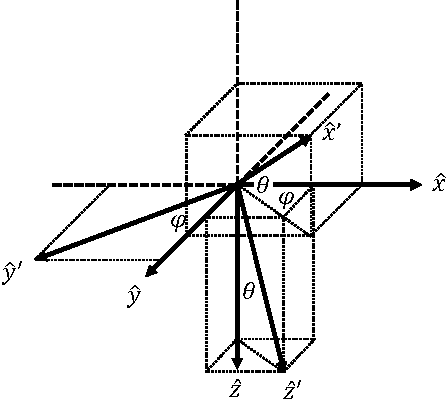
\includegraphics[scale=1.0]{coordinate_systems-crop.pdf}
\caption{Definition of the beam coordinate system $(\hat{x}', \hat{y}',
\hat{z}')$ and the target coordinate system $(\hat{x}, \hat{y}, \hat{z})$ by
tilt angle $\theta$ and rotation angle $\varphi$.}
\label{fig:coord}
\end{figure}   
%
The \textbf{initial direction} of the ions is defined by a reference direction
and, optionally, an additional rotation due to beam  divergence.
The reference direction is defined by a tilt and a rotation angle relative to
the target coordinate system, see Fig.~\ref{fig:coord}. The tilt and rotation
angles may be specified, or the rotation angle may be chosen randomly for each
ion. Without beam divergence the initial directions of all ions coincide with
the reference direction $\hat{z}'$ (cf.\ Fig.~\ref{fig:coord}). Considering a
beam divergence means to randomly rotate the ion’s direction of motion on the
unit sphere from the beam direction in such a way that the probability per solid
angle follows a given distribution. Two beam divergence models may be chosen from:
isotropic within a maximum rotation angle and Gaussian with given standard
deviations in $\hat{x}'$ and $\hat{y}'$ direction.

\begin{figure}[htbp]
\centering
\noindent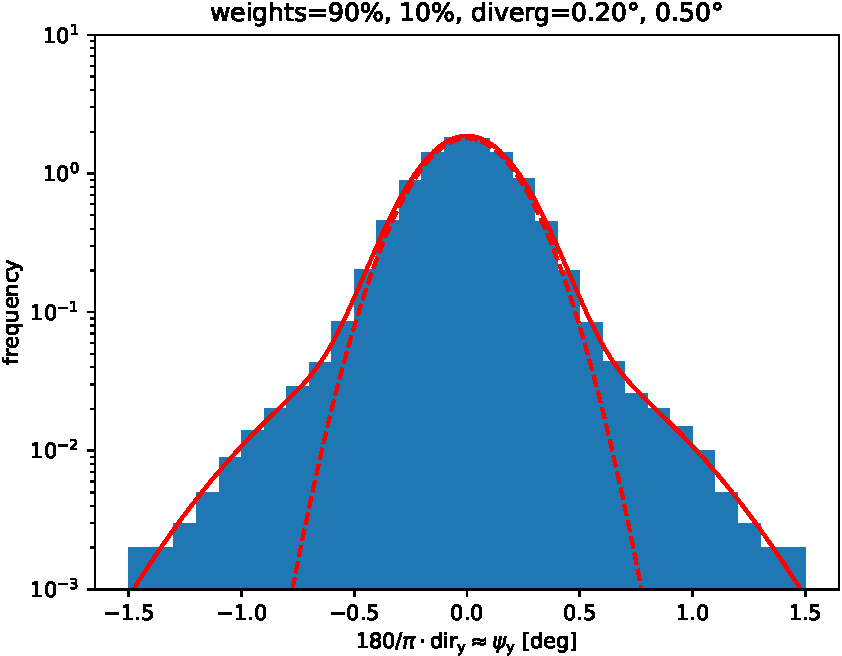
\includegraphics[scale=0.8]{diverg_y-crop.pdf}
\caption{Beam profile composed of two Gaussian functions (red line) and
histogram of angles \(\psi_\mathrm{y}\) generated by IMSIL.}
\label{fig:diverg}
\end{figure}  
%
More refined beam profiles or divergence distributions may be defined by
superposing partial beams using the \texttt{BEAM} index variable. An index
variable used on an input record specifies that the parameters on this record
apply to a particular object only, in this case to a partial beam. Each partial
beam may have a different beam profile and/or beam divergence. Ions are then
chosen with probabilities proportional to a specified beam weight from each of
the partial beams. An example for the superposition of two Gaussian beam
divergence distributions is shown in Fig.~\ref{fig:diverg}. Below is an excerpt
from an IMSIL input file that specifies the above beam profile: 
%
\begin{verbatim}
   &IONS NAME='B' ENERGY=5000 DOSE=1e13 TILT=0 MODDIV=2 NION=10000 /
   &IONS BEAM=1 WEIGHT=0.9 DIVERG=0.1,0.2 /
   &IONS BEAM=2 WEIGHT=0.1 DIVERG=0.2,0.5 /
\end{verbatim}
%
Note that parameters that are specified on the first line, which does not have
the \texttt{BEAM} index parameter, apply to both beams.

The \textbf{ion dose} may either be specified in ions per area in the $x$-$y$
plane (areal dose, units cm$^{-2}$), ions per length in $y$ direction (line
dose, units cm$^{-1}$), or ion count. The most natural choice among these
options depends on the dimensionality of the spatial histograms that are
computed: areal dose for 1-D, line dose for 2-D, and number doses for 3-D
histograms. However, other choices are possible, see Sections~\ref{s:his1d},
\ref{s:his2d}, and \ref{s:his3d}.

\begin{center}
\begin{tabular}{lll}
parameter \quad              & IMSIL name      & to be specified in record \\
\hline
internal starting point flag & \texttt{LIINIT}    & \texttt{\&IONS} \\
ion name                     & \texttt{NAME}      & \texttt{\&IONS} \\
energy                       & \texttt{ENERGY}    & \texttt{\&IONS} \\
atom mass                    & \texttt{MASS}      & \texttt{\&ATOMS} \\
reference starting point     & \texttt{XINIT}     & \texttt{\&IONS} \\
                             & \texttt{YINIT}     & \texttt{\&IONS} \\
                             & \texttt{ZINIT}     & \texttt{\&IONS} \\
beam FWHM                    & \texttt{FWHM}      & \texttt{\&IONS} \\
tilt angle                   & \texttt{TILT}      & \texttt{\&IONS} \\
rotation angle               & \texttt{ROTATE}    & \texttt{\&IONS} \\
random rotation flag         & \texttt{RANROT}    & \texttt{\&IONS} \\
beam divergence model        & \texttt{MODDIV}    & \texttt{\&IONS} \\
beam divergence              & \texttt{DIVERG}    & \texttt{\&IONS} \\
beam index variable          & \texttt{BEAM}      & \texttt{\&IONS} \\
beam weight                  & \texttt{WEIGHT}    & \texttt{\&IONS} \\
dose                         & \texttt{DOSE}      & \texttt{\&IONS} \\
dose units                   & \texttt{DOSEUNITS} & \texttt{\&IONS} \\
number of simulated ions     & \texttt{NION}      & \texttt{\&IONS} \\
\end{tabular}
\end{center}

%
\section{Material}
\label{s:mater}
For \textbf{static simulations}, the target is composed of \textbf{regions}.
Each region is described by a material and a geometry. The \textbf{material} is
primarily defined by its name, which is a chemical formula similar to the ion
name. The \textbf{density} of a region is set to the weighted densities of the
elementary materials by default, or can be specified by the user. Note that for
compound targets, the weighted densities are often inaccurate, so their
densities should be specified in the input file. 

Another material property is its \textbf{crystallinity}. If the material is
crystalline, the crystal structure is defined in the \texttt{CRYSTAL} record. In
addition, the crystallographic directions of the surface normal and of a surface
vector may be specified. Alternatively, the material may be specified as
polycrystalline, in which case a new random orientation of the crystal is chosen
for each ion. 

A further material property is the RMS \textbf{thermal vibration} amplitude of
the atoms, which may either be calculated from the Debye theory using the target
and Debye temperature, or it may be specified directly. Thermal vibrations are
only relevant in crystalline targets.

For \textbf{dynamic simulations}, the \texttt{\&MATERIAL} record can be used to
specify the initial material name and density. These specifications are
converted into atom densities, which are used to initialize the cell contents.
The cell densities are then allowed to change during the simulation. Since the
other material properties depend on the target composition, they can only be 
interpolated from the elemental material properties. Crystalline targets are not
allowed in dynamic simulations. 


\begin{center}
\begin{tabular}{lll}
parameter \quad                 & IMSIL name    & to be specified in record \\
\hline
number of regions               & \texttt{NR}        & \texttt{\&SETUP} \\
material name                   & \texttt{NAME}      & \texttt{\&MATERIAL} \\
elementary material density     & \texttt{DENSITY}   & \texttt{\&ATOMS} \\
material density                & \texttt{DENSITY}   & \texttt{\&MATERIAL} \\
crystallinity flag              & \texttt{XTAL}      & \texttt{\&MATERIAL} \\
polycrystallinity flag          & \texttt{LPOLY}     & \texttt{\&MATERIAL} \\
surface normal                  & \texttt{WAFER}     & \texttt{\&MATERIAL} \\
surface vector                  & \texttt{VSURF}     & \texttt{\&MATERIAL} \\
target temperature              & \texttt{TEMP}      & \texttt{\&SETUP} \\
Debye temperature               & \texttt{TDEBYE}    & \texttt{\&MATERIAL} \\
RMS thermal vibration amplitude & \texttt{VIB}       & \texttt{\&MATERIAL} \\

\end{tabular}
\end{center}

%
\section{Geometry}
\label{s:geometry}
IMSIL currently supports 1-D, 2-D, and 3-D geometries for
static simulations, and 1-D geometries for dynamic simulations. Static 
simulations may also use rotational symmetry to simplify geometry defnition
and/or accelerate simulation. 

\textbf{1-D geometries} describe layered targets with surfaces and interfaces
parallel to the $x$-$y$ plane. They are therefore defined by an array of $z$
coordinates which correspond to the position of the top surface, any
interfaces between layers (regions), and the bottom surface. Semi-infinite and
infinite targets may be approximated by large enough values of the surface
coordinates. 

1-D geometries combined with \textbf{cylindrical or spherical symmetry} describe
targets composed of cylindrical or spherical shells. The surface and interface
positions then refer to the distance from the symmetry line or center. The
``top'' surface is the inner surface, and the ``bottom'' surface the outer
surface. If a hollow body is not desired, the position of the inner surface has
to be assigned a negative value.

During a \textbf{dynamic simulation}, the cell densities are allowed to change
until some threshold is reached for the deviation from equilibrium. Then the
cell geometries are adapted so that the densities relax towards equilibrium. For
further details see Section~\ref{s:updates}.

\textbf{2-D geometries} are defined by polygons in the $x$-$z$ plane. The
polygons are defined by vertices and their connectivity (for details see
Section~\ref{s:geom}). Since these specifications can be lengthy, they can be
put into a separate geometry file. 2-D geometries also may be specified to be
periodic in $x$ direction. Internally, the geometry information is converted
into a signed distance function array for each region. The distance values are 
defined on a regular mesh covering the respective region.

\textbf{3-D rotational symmetric geometries} may be realized by combining 2-D
geometries with cylindrical symmetry. For a symmetry axis parallel to the $x$
axis, the 3-D geometry is defined by rotating the polygons about this axis.
Other orientations of the symmetry axis are realized by permutations of $x$,
$y$, and $z$ \cite{bradley_second_2021}.

2-D and arbitrary 3-D geometries may also be defined by signed distance function
(SDF) values on a regular grid, provided as external input on files. An SDF 
specifies the distance of the grid points from the nearest point on the
boundary of the region under consideration. It is given a negative sign
when the grid point is outside the region. An SDF must also be provided 
for the whole simulations domain (= the union of all regions) including a rim
of thickness at least equal to the maximum free flight path. (?) All region
SDFs must provide values on the whole simulation domain. Currently, 
the user is responsible for the consistency of the SDFs.

Finally, a simple \textbf{surface roughness} model is provided for both 1-D and
2-D simulations. This so-called density gradient model
\cite{lindsey_simple_2017} reduces the target density linearly towards the
surface in a sub-surface layer. The model has been introduced to provide more
realistic sputter yields at glancing incidence. 


\begin{center}
\begin{tabular}{lll}
parameter \quad                   & IMSIL name    & to be specified in record \\
\hline
number of regions                 & \texttt{NR}      & \texttt{\&SETUP} \\
dimensionality                    & \texttt{NDIM}    & \texttt{\&SETUP} \\
1-D surface/interface coordinates & \texttt{POSIF}   & \texttt{\&GEOMETRY} \\
cylindrical symmetry flag         & \texttt{LCYLX}   & \texttt{\&GEOMETRY} \\
                                  & \texttt{LCYLY}   & \texttt{\&GEOMETRY} \\
                                  & \texttt{LCYLZ}   & \texttt{\&GEOMETRY} \\
spherical symmetry flag           & \texttt{LSPHER}  & \texttt{\&GEOMETRY} \\
position of symmetry line/center  & \texttt{CENTER}  & \texttt{\&GEOMETRY} \\
2-D geometry file                 & \texttt{GEOMFILE} & \texttt{\&GEOMETRY} \\
polygon vertices                  & \texttt{POS}     & \texttt{\&GEOMETRY} \\
polygon connectivity              & \texttt{POINTS}  & \texttt{\&GEOMETRY} \\
periodicity flag                  & \texttt{LPERX}   & \texttt{\&GEOMETRY} \\
periodic boundary positions       & \texttt{XPER}    & \texttt{\&GEOMETRY} \\
box width of distance grid        & \texttt{WBOX2}   & \texttt{\&GEOMETRY} \\
maximum size of distance grid     & \texttt{NBOX2}   & \texttt{\&GEOMETRY} \\
signed distance function file     & \texttt{SDFFILE} & \texttt{\&GEOMETRY} \\
thickness of roughness layer      & \texttt{WROUGH}  & \texttt{\&GEOMETRY} \\

\end{tabular}
\end{center}

%
%%%%%%%%%%%%%
% Chapter 3 %
%%%%%%%%%%%%%
%
\chapter{Physical Models}
\label{k:phys}
In this chapter an overview of the physical models implemented in IMSIL 
is given. More details are found in the references listed at the end of
this manual. A particular objective of this chapter is to give 
correspondence lists of the notation of the most important model 
parameters as used in this chapter or in the references and the names of 
the variables as they have to be specified in the input file. The complete 
information about all input parameters is found in Chapter~\ref{k:input}.

%
\section{Selection of Collision Partners}
\label{s:coll}
\ifprivate
Aside from being a binary collision simulator, IMSIL also has a
simplified molecular dynamics mode which treats the ion target
interaction by integration of the equations of motion of the moving
particles. It is simplified inasmuch as only interations between the
ion or recoil and the target atoms are taken into acoount and
interactions among the target atoms are disregarded. Also, it is
restricted to simulations in a single crystalline layer, and no
lattice damage may be taken into account. Nevertheless, the user is
given access to this mode by the \texttt{LMD} flag. There are only a
few parameters specific to the MD mode, such as the accuracy of time
integration, which are hard-coded. For more information and
applications see \cite{I9701,I0101}. 
\fi

In the binary collision approximation, the collisions are treated as if the ions
interacted with only one target atom at a time.  In \textbf{amorphous} targets,
the algorithm used is similar to that implemented in TRIM \cite{I8001}, however,
with a different choice of the maximum impact parameter. $p_\mathrm{max}$ is
calculated depending on energy and ion and target atom species, based on two
criteria \cite{hobler_acceleration_1995}. The energy transfer criterion
guarantees that scattering events with energy transfers larger than a
user-specified value $T_\mathrm{min}$ are taken into account. The scattering
angle criterion guarantees that all scattering events with scattering angles
larger than the user-specified value $\psi_\mathrm{min}$ are taken into account.
The resulting  $p_\mathrm{max}$ values are limited by $p_\mathrm{max,max}$ and
$p_\mathrm{max,\psi}$, respectively. The larger of the maximum impact parameters
determined from the two criteria is taken. In addition, the impact parameter is
forced to be at least $p_\mathrm{max,min}$. It is possible to use a fixed
maximum impact parameter by setting all of $p_\mathrm{max,max}$,
$p_\mathrm{max,\psi}$, and $p_\mathrm{max,min}$ to the desired value. 

The user can choose between a deterministic and a random free flight path. The
latter assumes an exponential probability density function with a mean value
equal to the deterministic free flight path. The (mean) free flight path
$\overline{L}$ is calculated from the relation 
$\overline{L} \cdot \pi p_{max}^2 = N^{-1}$, which considers the correct atomic 
density $N$ of the target. As usual \cite{I8001}, the square of the impact
parameter $p$ is selected randomly with a uniform distribution between 0 and 
$p_{max}^2$, and the azimuthal position of the target atom with respect to the 
ion path is chosen randomly between 0 and $2\pi$. 

In a \textbf{crystalline} target region, after each collision, the next target
atom to be hit has to be selected from the lattice positions surrounding the 
ion. This is done among all lattice sites that lead to impact parameters
$p < p_\mathrm{max,c}$ and free flight paths $0 < L < L_\mathrm{max,c}$. In
addition, to limit the size of the search cell, only atoms with a distance from
the projectile less than the search distance $r_\mathrm{min,c}$ are guaranteed
to be checked. For consistency, the following condition must hold:
%
\begin{equation}
   L_\mathrm{max,c}^2 + p_\mathrm{max,c}^2 \le r_\mathrm{min,c}^2   
   \label{eq:search}
\end{equation}
%
For the diamond crystal structure, it is usually not necessary to change the
default values of these parameters. If it is done, it is important to obey
Eq.~(\ref{eq:search}). For other crystal structures, it might be essential to
set $p_\mathrm{max,c}$ in the input file. With larger $p_\mathrm{max,c}$, more
distant collision partners are taken into account, which might increase accuracy
at low energies on the expense of increasing computation times. Too small
$p_\mathrm{max,c}$ might introduce inaccuracies into the simulation. For crystal
structures other than the default diamond structure, $r_\mathrm{min,c}$ is
calculated by the program. The choice of $L_\mathrm{max,c}$ is uncritical, it
only affects the computational efficiency.

The default values of $p_\mathrm{max,\psi}$ and $p_\mathrm{max,c}$ are implant
energy dependent for energies less than $10$~keV in order to allow more accurate
simulation of low-energy implantations.

Small displacements from the lattice positions due to thermal vibrations are
taken into account. These are assumed to be uncorrelated and distributed
according to a Gaussian function. The RMS displacement in one direction,
$x_\mathrm{rms}$, may be calculated using the Debye theory \cite{I7403}. A value
of 490~K is recommended for the Debye temperature of Si
\cite{hobler_role_1993,hobler_verification_1996}. The values of the Debye
temperatures for all elements are tabulated within IMSIL and appropriate
vibrational amplitudes are calculated using the Debye function \cite{I7403}.

It has been shown that ``simultaneous collisions'' are not beneficial
for dopant profile calculation \cite{hobler_study_1997,
hobler_modeling_1997,hobler_useful_2001}. ``Simultaneous collisions'' refer to
an algorithm which treats collisions with several target atoms simultaneously,
when the collisions are separated by a free flight path smaller than a (small)
value $L_\mathrm{sim}$ \cite{I7401}. This treatment can only be approximate,
since the three-body problem cannot be solved exactly, as is known from
classical mechanics. To our experience, no improvement can be obtained by using
``simultaneous collsions''. This feature has therefore been eliminated from
IMSIL.  The quality of the treatment of collisions in crystalline targets is
also supported by the good results obtained in round robin simulations
\cite{gartner_round_1995} and other comparisons with MD simulations
\cite{schlueter_absence_2020,hobler_channeling_2019}.

The motion of the ions near \textbf{interfaces} between regions and between
a region and vacuum is carefully treated. For this purpose, when the ion moves
near to an interface, potential collision partners from both adjoining regions
are considered.  This is particularly important for dynamic simulations
(\texttt{LDYN=T}) where the composition and density of the target may change
from cell to cell with the cells typically being quite small.  In a dynamic
simulation, the implanted ions are recorded and taken into account as potential
collision partners for subsequent ions and recoils.
%%% we need a more extended description of the dynamic mode, otherwise
%%% it might be difficult to set up an input file

\begin{center}
\begin{tabular}{lll}
parameter \quad    & IMSIL name     & to be specified in record \\
\hline
\ifprivate
MD mode flag            & \texttt{LMD}  & \texttt{\&SETUP} \\
\fi
dynamic simulation flag & \texttt{LDYN}     & \texttt{\&SETUP} \\
$\psi_\mathrm{min}$     & \texttt{PSIFFP}   & \texttt{\&SNPAR} \\
$T_\mathrm{min}$        & \texttt{DENFFP}   & \texttt{\&SNPAR} \\
$p_\mathrm{max,min}$    & \texttt{PMAXMIN}  & \texttt{\&SNPAR} \\  
$p_\mathrm{max,max}$    & \texttt{PMAXMAX}  & \texttt{\&SNPAR} \\  
$p_\mathrm{max,\psi}$   & \texttt{PMAXPSI}  & \texttt{\&SNPAR} \\  
$N$                     & \texttt{DENSITY}  & \texttt{\&MATERIAL} \\
$p_\mathrm{max,c}$      & \texttt{PMAX}     & \texttt{\&CRYSTAL} \\
$L_\mathrm{max,c}$      & \texttt{FFPMAX}   & \texttt{\&CRYSTAL} \\
$r_\mathrm{min,c}^2-1$  & \texttt{NRAD2}    & \texttt{\&CRYSTAL} \\
$x_\mathrm{rms}$        & \texttt{VIB}      & \texttt{\&MATERIAL} \\

\end{tabular}
\end{center}

%
\section{Interatomic Potential}
\label{s:pot}
The standard model of the interatomic potential used in IMSIL is the 
universal ZBL potential \cite{I8512}. It reads 
%
\begin{equation}
   V(r) = \frac{Z_1 Z_2 e^2}{r} \cdot \Phi(\frac{r}{a_{12}}), \qquad
   \Phi(R) = \sum_{i=1}^4 a_i \cdot \exp(-b_i R)
   \label{eq:ZBLfun}
\end{equation}
%
$Z_1$ and $Z_2$ denote the atomic numbers of the ion and the target atom, 
respectively, $r$ the interatomic separation, and $a_{12}$ the screening length
%
\begin{equation}
   a_{12} = \frac{0.468~\mbox{\AA}}{Z_1^{0.23} + Z_2^{0.23}}
   \label{eq:ZBLscr}
\end{equation}
%
The coefficients of the screening function $\Phi$ are given by 
$a_i =~$\{0.1818, 0.5099, 0.2802, 0.02817\} and   
$b_i =~$\{3.2,    0.9423, 0.4029, 0.2016\} \cite{I8512}. The scattering angles
and the energy transfer from projectile to recoil are calculated, as usual, from
the scattering angle in the center-of-mass system $\theta$. In the default
model, $\theta$ is calculated by bicubic interpolation in tables of
$\cot(\theta/2)$ \cite{I8730}. Such tables may be set up, in principle, for any
interatomic potential. However, the screening length is assumed according to
Eq.~\ref{eq:ZBLscr} in any case. The scattering table file corresponding to the
universal ZBL potential is called \texttt{SCATTAB}.

The universal ZBL screening function has been obtained by averaging a large 
number of ``pair-specific'' interatomic potentials (i.e. for specific
projectile-recoil atom combinations) \cite{I8512}. Tables for some of the
pair-specific potentials are also provided with the program.

Alternatively, the scattering angle $\theta$ in the center-of-mass system can be 
determined by numerical integration using Gauss-Legendre or Gauss-Mehler
quadrature. The screening function may either be assumed as a sum of
exponentials (Eq.~\ref{eq:ZBLfun}) or may be defined by a table. Tables for the
screening functions of all pair-specific potentials are provided.

\begin{center}
\begin{tabular}{lll}
   parameter \quad & IMSIL name \qquad\qquad & to be specified in record \\
   \hline
   $Z_1$           & derived from ion name      & -- \\
   $M_1$           & derived from ion name or 
                     \texttt{MASS}              & \texttt{\&ATOMS} \\
   $Z_2$           & derived from material name & -- \\
   $M_2$           & derived from material name or
                     \texttt{MASS}              & \texttt{\&ATOMS} \\
   scattering 
   table file      & \texttt{SCATFILE}          & \texttt{\&SNPAR} \\
   screening
   coefficients    & \texttt{COEFFILE}          & \texttt{\&SNPAR} \\
   screening 
   function table  & \texttt{SCRFILE}           & \texttt{\&SNPAR} \\
\end{tabular}
\end{center}

The format of the files \texttt{SCATFILE}, \texttt{COEFFILE}, and 
\texttt{SCRFILE} is described in Section~\ref{s:input}. 


%
\section{Implantation Damage}
\label{s:dam}
The number of atoms displaced from their lattice sites may be calculated
in IMSIL either using the modified Kinchin-Pease model \cite{I7504} or by
following the recoils. In the latter case, the recoils may be followed 
until they come to rest, or until their energy falls below a user-defined
value $E_\mathrm{lim}$. When the recoil energy falls below $E_\mathrm{lim}$, the
number of interstitials $\nu_\mathrm{gen}$ generated in the remaining part of its 
collision cascade is calculated by the modified Kinchin-Pease model.

In a recoil cascade, when the energy transfered to a target atom (recoil)
exceeds its displacement energy $E_\mathrm{d}$, it is set into motion, and a
vacancy is generated (which may be subject to recombination). When the recoil
comes to rest, an interstitial is generated (which may be subject to
recombination as well), unless it produces a recoil of the same type in its last
collision (this is called a ``replacement collision'').  

Recombination with point defects generated within the same recoil 
cascade is treated by the recombination factor $f_\mathrm{rec}$.
Recombination with point defects generated by previous recoil cascades is
taken into account with a probability proportional to the point defect 
concentration. When the recoil motion is followed until the end of the 
trajectory, the damage increments are calculated in the following way
\cite{hobler_net_1996}: 
%
%
\begin{enumerate}
\item[(i)]
When an interstitial is recoiled, the local interstitial number decreases
by one. No other processes are assumed to be induced.
%
\begin{equation}
   \Delta n_\mathrm{I} = - 1 \qquad \Delta n_\mathrm{V} = 0
\end{equation}
%
\item[(ii)]
When a lattice atom is recoiled, the model takes into account defect 
recombination both with interstitials generated within the same 
cascade (described by $f_\mathrm{rec}$) and with interstitials originating from 
previous cascades (described by the probability $1-kN_\mathrm{I}$ that the 
vacancy is not located within the capture radius of an interstitial). 
%
\begin{equation}
   \Delta n_\mathrm{V} = f_\mathrm{rec} (1-kN_\mathrm{I}) \qquad 
   \Delta n_\mathrm{I} = \Delta n_\mathrm{V} - 1
   \label{eq:rgl}
\end{equation}
%
The second relation is implied by the conservation of particle numbers
during recombination.
%
\item[(iii)]
When a recoil comes to rest, it is only allowed to recombine with vacancies 
from previous cascades (described by the factor $1-kN_\mathrm{V}$), 
but not with those of the same cascade. The latter 
would mean to count recombination processes within the recoil cascade twice
and has to be excluded therefore.
%
\begin{equation}
   \Delta n_\mathrm{I} = 1-kN_\mathrm{V} \qquad 
   \Delta n_\mathrm{V} = \Delta n_\mathrm{I} - 1
   \label{eq:rs}   
\end{equation}
%
\end{enumerate}
%
$k$ is set equal to $1/N_\mathrm{sat}$ if recombination with defects from 
previous cascades is assumed to take place, where $N_\mathrm{sat}$ denotes the
saturation density of the point defects. $k=0$ is used otherwise. Notice that
$n$ denotes defect numbers, while $N$ denotes defect concentrations.

The above formulae assume that the additional Frenkel pairs described by
$f_\mathrm{rec}$ are generated where a lattice atom is recoiled. It
is also possible that part or all of the additional Frenkel pairs are
generated where the recoil stops. Introducing the fraction of these
additional Frenkel pairs generated at the starting point of the recoil
trajectory as the parameter $f_\mathrm{rg}$, Eqs.~(\ref{eq:rgl}) and 
(\ref{eq:rs}) are replaced by
%
\begin{equation}
   \Delta n_\mathrm{V} = (1 - f_\mathrm{rg} + f_\mathrm{rg} f_\mathrm{rec}) 
   (1-kN_\mathrm{I}) \qquad 
   \Delta n_\mathrm{I} = \Delta n_\mathrm{V} - 1
   \label{eq:rgl2}
\end{equation}
%
and
%
\begin{equation}
   \Delta n_\mathrm{I} = (f_\mathrm{rg} + (1-f_\mathrm{rg}) f_\mathrm{rec})
   (1-kN_\mathrm{V}) \qquad 
   \Delta n_\mathrm{V} = \Delta n_\mathrm{I} - 1
   \label{eq:rs2}   
\end{equation}
%
respectively. Note that these equations reduce to Eqs.~(\ref{eq:rgl}) and 
(\ref{eq:rs}) for $f_\mathrm{rg}=1$.


When the modified Kinchin Pease model is used to calculate the number of point
defects generated in the remaining subcascade, a formula based on the above
assumptions is used taking the probability of the three events into account.%
\footnote{The formula is similar to  
%
\begin{displaymath}
   \nu_\mathrm{st} = \nu_\mathrm{gen} \cdot f_\mathrm{rec} \cdot
      (1 - N_\mathrm{V} / N_\mathrm{sat} )
\end{displaymath}
%
which was used in earlier versions of IMSIL. $\nu_\mathrm{st} (= 
\Delta n_\mathrm{I} = \Delta n_\mathrm{V})$ denotes the average number of 
stable point defects.}

Values of $f_\mathrm{rec}$ larger than unity indicate that there is in
fact no damage recombination but rather damage multiplication due to
nonlinear effects. Damage recombination and damage saturation are
usually observed only for light ions. IMSIL also offers the possibility to turn
the target into the amorphous state when the damage density exceeds a user
specified value $N_\mathrm{amo}$.

Values of $f_\mathrm{rec}$, $N_\mathrm{sat}$, $N_\mathrm{amo}$ have been
determined for B \cite{hobler_boron_1995}, P \cite{hobler_net_1996,
herzog_monte_1995}, As \cite{hobler_net_1996, simionescu_modeling_1995}, and
BF$_2$ \cite{hobler_net_1996, simionescu_monte_1995} in Si. Further
investigations of the damage model are reported in
\cite{hobler_verification_1996, simionescu_comparison_1995}. Regarding B in Si, 
investigation of ultra-low energy B implants led to the conclusion that a
higher value of $f_\mathrm{rec}$ and no damage saturation is preferable at low energies
\cite{hobler_modeling_1997}. These values are also  consistent with the dose
dependence of higher-energy implantations in (100)-Si. The default values in
IMSIL have been adjusted accordingly. It should be noted, however, that one
should revert to the values given in \cite{I9504} if the dose dependence of
[110] channeling is investigated. 

The model may also be used in a simplified version that does not consider
defect recombination with previous cascades, corresponding to $k=0$ and/or
$N_\mathrm{I}=N_\mathrm{V}=0$. It is also possible that the damage 
distributions are only updated after a certain number of cascades. 

As an alternative in case of true recombination ($f_\mathrm{rec} < 1$), the
capture radius model may be used \cite{simionescu_comparison_1995}. In this
model the positions of vacancies and interstitials generated in each collision
cascade are stored, and vacancies and interstitials that are within a capture
radius $r_\mathrm{cap}$ are annihilated. 

As an alternative in case of damage multiplication ($f_\mathrm{rec} > 1$), the
amorphous pocket model may be used \cite{hobler_amorphous_2003}: In this
model, each energy deposition event is assigned a sphere the volume of which
would be molten according to the heat of fusion (0.52 eV/atom in Si), if surface
effects could be excluded. After each collision cascade, the connected volume
of overlapping melting spheres are determined. Each such overlapping area defines
an amorphous pocket candidate. The number of displaced atoms associated with it 
is the ratio of the sum of energies deposited by their members and the heat
of fusion. Surface effects are taken into account by shrinking the amorphous 
pocket candidate by a certain amount. If the remaining pocket meets a minimum 
size requirement, an amorphous pocket is generated with the number of displaced 
atoms calculated as indicated above. Otherwise the amorphous pocket candidate is
abandoned, and the interstitials contained in it are used to calculate the
number of displaced atoms. 

In addition to the above model, an ion beam induced interfacial amorphization
(IBIIA) model \cite{I9766} can be activated. In this model, existing amorphous
zones grow with a rate proportional to nuclear energy deposition.

In addition to being recorded, damage to crystalline regions can also be
considered in the selection of collision partners.

\begin{center}
\begin{tabular}{lll}
   parameter \quad  & IMSIL name & to be specified in record \\
   \hline
   flag for considering defect recombination  &                               \\
   with previous cascades and using damage in & {\tt LDAMDYN}& {\tt \&SETUP}  \\
   crystalline regions                        &                               \\
   damage update interval                     & {\tt NIONHIS}& {\tt \&SETUP} \\
   refined damage model flag                  & {\tt LDAM}   & {\tt \&DAMAGE} \\
   displacement energy $E_\mathrm{d}$         & {\tt ED}     & {\tt \&DAMAGE} \\
   recoil cutoff energy $E_\mathrm{lim}$      & {\tt ELIMKP} & {\tt \&DAMAGE} \\
   replacement collision flag                 & {\tt LREPL}  & {\tt \&DAMAGE} \\
   recombination fraction $f_\mathrm{rg}$     & {\tt FRACRG} & {\tt \&DAMAGE} \\
   damage recombination factor $f_\mathrm{rec}$ & {\tt FREC} & {\tt \&DAMAGE} \\
   damage saturation density $N_\mathrm{sat}$ & {\tt DAMSAT} & {\tt \&DAMAGE} \\
   amorphization threshold $N_\mathrm{amo}$   & {\tt DAMAMO} & {\tt \&DAMAGE} \\
   capture radius model flag                  & {\tt LCAP}   & {\tt \&DAMAGE} \\
   capture radius                             & {\tt RCAP}   & {\tt \&DAMAGE} \\
   amorphous pocket model flag                & {\tt LPOCK}  & {\tt \&DAMAGE} \\
   heat of fusion                             & {\tt EMELT}  & {\tt \&DAMAGE} \\
   amorphous pocket shrink parameter          & {\tt FPOCK}  & {\tt \&DAMAGE} \\
   minimum pocket size                      & {\tt NPOCKMIN} & {\tt \&DAMAGE} \\
   IBIIA model flag                           & {\tt LIBIIA} & {\tt \&DAMAGE} \\
   IBIIA growth rate constant                 & {\tt RIBIIA} & {\tt \&DAMAGE} \\
\end{tabular}
\end{center}

%
\section{Backscattering, Transmission, and Sputtering}
\label{s:sput}
Ions leaving the target on the same side as they entered it, are called
\textbf{backscattered} or reflected. Ions leaving a membrane on the opposite
side of where they entered it, are called transmitted. In a conventional 1-D
membrane setup, the ions impinge on the top surface (lowest $z$ coordinate of the
target) and may be emitted from that surface with a negative $z$ component of
their direction of motion. Conversely, if they are emitted from the bottom
surface, they have a positive $z$ component of their direction of motion. IMSIL
takes the sign of the $z$ component of the direction of motion as the criterion
for distinguishing between ``backscattered'' and ``transmitted'' atoms. Note
that this distinction may not always make sense, e.g., when ions can be emitted
from the sides of a 2-D or 3-D target. In those cases it might be more
reasonable to just add backscattered and transmitted ions.

Target atoms that are followed as recoils and leave the target, are called
\textbf{sputtered}. They are also classified into backscattered and transmitted
recoils, which corresponds to backward and forward sputtered atoms. There is no
difference in treating ions and recoils with respect to their leaving the
target. Therefore, their statistics is alway reported alongside.

When accurate sputtering characteristics are desired, the ``accurate sputtering
flag'' should be set. Then recoils are followed down to the surface binding
energy $E_\mathrm{surf}$ rather than down to the displacement energy
$E_\mathrm{d}$, if they are closer to the surface than some distance
$d_\mathrm{near}$. Within this distance, recoils with energies less than the
displacement energy are followed as ``virtual'' recoils. Virtual recoils deposit
energy like real recoils and are counted as sputtered when they leave the
target, but they generate defects (vacancies at the starting point, and
interstitials at the end point if the recoil reenters the target) only when they
leave the target.
  
With the accurate sputtering flag set, also the maximum impact parameter
$p_\mathrm{max}$ is adjusted in the near-surface zone such that no collisions
with energy transfer larger than the surface binding energy are missed.

When the ions enter the target, they gain the surface binding energy, and ions
and recoils loose the surface binding energy when they are emitted. Depending on
the model of the potential barrier, they may also be refracted. A planar
potential barrier \cite{I6909} is usually a good choice and is therefore the
default. The potential barrier model can be changed to isotropic, where there is
no refraction, or to an intermediate model \cite{hobler_assessment_2013} using a
``nonplanarity parameter''.

When a recoil reaches the surface with an energy not sufficient to surmount the
potential barrier, it is reflected. With the planar potential model, it may
happen that the recoil bounces back and forth beween the barrier (which is
at $p_\mathrm{max}$ outside the target) and the target. The number of
reflections may be limited.

\begin{center}
\begin{tabular}{lll}
   parameter \quad          & IMSIL name & to be specified in record \\
   \hline
   accurate sputtering flag                 & {\tt LSPUT}   & {\tt \&SETUP} \\
   surface binding energy $E_\mathrm{surf}$ & {\tt ESURF}   & {\tt \&DAMAGE} \\
   displacement energy $E_\mathrm{d}$       & {\tt ESURF}   & {\tt \&DAMAGE} \\
   $d_\mathrm{near}$                        & {\tt DNEAR}   & {\tt \&DAMAGE} \\
   nonplanarity parameter                   & {\tt KSURF}   & {\tt \&DAMAGE} \\
   maximum number of reflections         & {\tt REFLECTMAX} & {\tt \&DAMAGE} \\
\end{tabular}
\end{center}


%
\section{Electronic Stopping}
\label{s:stop}
The electonic stopping of channeled ions is reduced as compared with ions 
moving in a random direction. This may be taken into account by an impact 
parameter dependent model. The model implemented in IMSIL is composed of a part
which is proportional to the path length $L$
%
\begin{equation}
   \Delta E_\mathrm{e}^\mathrm{nl} = 
      N \cdot S_\mathrm{e} \cdot L \cdot
      \left[ x^\mathrm{nl} + x^\mathrm{loc} \cdot 
      \left( 1 + \frac{p_\mathrm{max}}{a} \right)
             \cdot \exp \left\{ - \frac{p_\mathrm{max}}{a} \right\} \right]
   \label{eq1}
\end{equation}
%
and a part which depends on the impact parameter $p$ 
%
\begin{equation}
   \Delta E_\mathrm{e}^\mathrm{loc} = 
      x^\mathrm{loc} \cdot \frac{S_\mathrm{e}}{2 \pi a^2} \cdot
      \exp \left\{ - \frac{p}{a} \right\}
   \label{eq2}
\end{equation}
%
$N$ denotes the atomic density of the target. The impact parameter dependence
is according to Oen and Robinson \cite{I7607}. Alternatively, the impact 
parameter dependence can be chosen by a generalized Firsov model \cite{I5901}, 
in which case the model reads
%
\begin{equation}
   \Delta E_\mathrm{e}^\mathrm{nl} = 
      N \cdot S_\mathrm{e} \cdot L \cdot
      \left[ x^\mathrm{nl} + x^\mathrm{loc} \cdot \frac{
      1 + (d-1) \frac{p_\mathrm{max}}{a}}{
      \left( 1 + \frac{p_\mathrm{max}}{a} \right) ^ {d-1}} \right]
   \label{eq1a}
\end{equation}
%
and
%
\begin{equation}
   \Delta E_\mathrm{e}^\mathrm{loc} = 
      x^\mathrm{loc} \cdot \frac{S_\mathrm{e}}{2 \pi a^2} \cdot
      (d-1) (d-2) \left( 1 + \frac{p}{a} \right) ^ {-d}
   \label{eq2a}
\end{equation}
%
In the original Firsov model $d=5$. We do not use Firsov's prefactor and
screening length. If desired, Firsov's values can be set by appropriate values
of $k/k_\mathrm{L}$ and $f$ (see below).

In Eqs.~(\ref{eq2}) and~(\ref{eq2a}), the distance of closest approach $r_0$ 
in the collision (apsis of the collision) may be used instead of the impact
parameter $p$. The most significant effect of this choice is a reduction in
electronic stopping at low energies.

$a$ is the screening length of the impact parameter dependent part, which 
is expressed by the value $a_\mathrm{OR}=a_\mathrm{ZBL}/0.3$ proposed by Oen and
Robinson \cite{I7607} with $a_\mathrm{ZBL}$ the screening length of the ZBL
interatomic potential \cite{I8512}.
%
\begin{equation}
   a = f \cdot a_\mathrm{OR} ~( = f \cdot a_{12} / 0.3 )
   \label{eq5}
\end{equation}
%

The random electronic stopping power $S_\mathrm{e}$ may be calculated in either
of two ways. In the first case (models \# 1 or \#3) it is assumed to be a power
of the ion energy
%
\begin{equation}
   S_\mathrm{e} = S_\mathrm{eL} = k \cdot E^p
   \label{eq3}
\end{equation}
%
With $p = 0.5$ this is Lindhard's model \cite{I6101}, where electronic stopping
is proportional to the ion velocity. In order to describe the electronic stopping
power for high-energy ions, in model \# 3 a formula similar to that of Biersack
\cite{I8001} is used \cite{simionescu_model_1995} 
%
\begin{equation}
   S_\mathrm{e} = \left( {S_\mathrm{eL}}^{-c} + 
                         {S_\mathrm{eB}}^{-c} \right) ^ {-1/c}
\end{equation}
%
where $S_\mathrm{eL}$ denotes the Lindhard like stopping power according to
Eq.~(\ref{eq3}) and $S_\mathrm{eB}$ the slightly modified Bethe Bloch stopping
power as described in \cite{I8001}:
%
\begin{equation}
   S_\mathrm{eB} = \frac{B}{E_\mathrm{b}} \cdot
      \ln \left( {E_\mathrm{b} + c_0 + \frac{c_1}{E_\mathrm{b}}}\right)
   \label{eq3a}
\end{equation}
%
where $B$ and $E_\mathrm{b}$ denote ion-target dependent prefactors. (For
details see \cite{I8001}).  In the second case (models \# 2 or \# 4) the ZBL
electronic stopping power \cite{I8512} is used. Alternatively, the random
electronic stopping power may also be read from a file.

$x^\mathrm{nl}$ and $x^\mathrm{loc}$ denote the nonlocal ($L$ dependent) and the
local ($p$ dependent) fraction of $S_\mathrm{e}$, respectively.
%
\begin{equation}
   x^\mathrm{nl} + x^\mathrm{loc} = 1
   \label{eq4}
\end{equation}
%
It has been found that the nonlocal fraction $x^\mathrm{nl}$ is energy
dependent. The energy dependence can be specified by specifying $x^\mathrm{nl}$
at different energies $E^\mathrm{nl}$. The actual values are interpolated
according to
%
\begin{equation}
   x^\mathrm{nl} \sim E^q
   \label{eq6a}
\end{equation}
%
(models \#1 and \#2), or
%
\begin{equation}
   x^\mathrm{nl} \sim S_\mathrm{e}(E) ^{2q}
   \label{eq6}
\end{equation}
%
(models \#3 and \#4) where $q$ is determined by the program from
$x^\mathrm{nl}$ values at two energies. Note that Eq.~(\ref{eq6}) reduces to
Eq.~(\ref{eq6a}) when the Lindhard like stopping power Eq.~(\ref{eq3}) is used. 
Default values of the parameters are provided by the program for all ions in
silicon \cite{hobler_monte_1995, hobler_towards_2000, hobler_boron_1995,
simionescu_modeling_1995, hobler_electronic_1993, hobler_random_2006}.
The value of $k$ is specified by a correction factor $k/k_\mathrm{L}$ to the
Lindhard stopping power. 

Electronic energy loss straggling may be considered according to Konac, Klatt,
and Kalbitzer \cite{hobler_random_2006, I9848}.

\begin{center}
\begin{tabular}{lll}
   parameter \quad & IMSIL name & to be specified in record \\
   \hline
   target density $N$                      & {\tt DENSITY} & {\tt \&MATERIAL} \\
   model number                               & {\tt MODEL}   & {\tt \&SEPAR} \\
   Lindhard correction factor $k/k_\mathrm{L}$ & {\tt CORLIN} & {\tt \&SEPAR} \\
   power $p$ in Lindhard stopping             & {\tt POWLIN}  & {\tt \&SEPAR} \\
   interpolation power $c$                    & {\tt POWINT}  & {\tt \&SEPAR} \\
   Bethe stopping constant $c_0$              & {\tt C0BETHE} & {\tt \&SEPAR} \\
   Bethe stopping constant $c_1$              & {\tt C1BETHE} & {\tt \&SEPAR} \\
   random electronic stopping file            & {\tt SEFILE}  & {\tt \&SEPAR} \\
   nonlocal fraction $x^\mathrm{nl}$          & {\tt XNL}     & {\tt \&SEPAR} \\
   energy for $x^\mathrm{nl}$, $E^\mathrm{nl}$  & {\tt ENL}   & {\tt \&SEPAR} \\
   screening length factor $f$                & {\tt FACSCR}  & {\tt \&SEPAR} \\
   Firsov $p$ dependence flag                 & {\tt FIRSOV}  & {\tt \&SEPAR} \\
   Firsov $p$ dependence power $d$            & {\tt POWFIRS} & {\tt \&SEPAR} \\
   apsis flag                                 & {\tt LAPSIS}  & {\tt \&SEPAR} \\
   electronic straggling flag                & {\tt STRAGGLE} & {\tt \&SEPAR} \\
   electronic straggling kink energy          & {\tt ESTRAG}  & {\tt \&SEPAR} \\
\end{tabular}
\end{center}

%
\section{Rutherford Backscattering / Channeling}
\label{s:RBS}
The code uses the principle of close encounter probability \cite{I7102} and
approximates the paths of the backscattered particles by straight trajectories
in a random medium. The program gives as the output the RBS signal as a function
of depth or backscattering energy. The nuclear encounter probability is the
cross section for the process times the integral of the product of the ion flux
and the probability of a target atom being at the point of passage.

The Rutherford backscattering cross section relates collision densities to
target atom densities. The probability of the collision is proportional to the
cross section area of the target sphere perpendicular to the path of the
projectile. The resulting probability that an ion will be scattered into a
detector with a given solid angle is represented in derivative form, the
derivative of the cross-section with respect to a differential solid angle
evaluated at a particular solid angle and projectile energy. The resulting
Rutherford differential cross section is given by:
%
 \begin{equation}
   \frac{\partial \sigma}{\partial \Omega}= 
   \left[\frac{Z_1 Z_2 e^{2}}{2 E} \right]^{2} 
   \cdot \frac {1}{\sin^{4}\psi} \cdot
   \frac{\left[\sqrt{1-{(\frac{m_1\cdot \sin\psi}{m_2}})^{2}} + \cos\psi \right]^{2}}
   {\sqrt{1-{(\frac{m_1\cdot \sin\psi}{m_2}})^{2}}}
   \label{rbs:eq1}
 \end{equation}
%
$e^2=1.44 \times 10^{-13}$~MeV$\cdot$cm is constant, $E$ and $m_1$ are the
energy and the mass of the incident ion, respectively, $m_2$ is the mass of the
target atom, and $\psi$ is the labaratory backscattering angle.  As the result
of a backscattering event, a particle will loose energy. The ratio of the
projectile energy immediately after scattering to the energy immediately before
scattering is the kinematic factor:
%
\begin{equation}
  K = \left[\frac{\sqrt{1-(\frac{m_1\cdot \sin\psi}{m_2})^{2}} 
      + \frac{m_1 \cdot \cos\psi }{m_2}}
    {1 + \frac{m_1}{m_2}} \right]^{2}
  \label{rbs:eq2}
\end{equation}
%
Atoms are assumed to vibrate independently, where the displacement probability 
is Gaussian distributed,
%
\begin{equation}
  P = \frac{1}{2 \pi x_\mathrm{rms}^{2}} \cdot \exp(-\frac{r^{2}}{2
  x_\mathrm{rms}^{2}}),
  \label{rbs:eq3}
\end{equation}
%
where $x_\mathrm{rms}$ denotes the RMS vibration amplitude of the target atoms
in one direction, and $r$ the distance vector between collision point and target
atom.  The energy detected in the detector (the backscattered energy) is
calculated by approximating the path of the backscattered particle by a
straight line in random medium.  The backscattering energy is scored in an
energy spectrum:
%
\begin{equation}
  P_\mathrm{RBS} = \frac{\partial \sigma}{\partial \Omega} \cdot P \cdot
  N_\mathrm{d}
  \label{rbs:eq4}
\end{equation}
%
where $N_\mathrm{d}$ is the ion dose. The units of \texttt{$P_\mathrm{RBS}$} are
cm$^{-2}$sr$^{-1}$.
%
\begin{center}
\begin{tabular}{lll}
   parameter \quad & IMSIL name & to be specified in record \\
   \hline
   backscattering angle $\psi$  & {\tt TILTA}   & {\tt \&OUTPUT}   \\
   dose $N_\mathrm{d}$          & {\tt DOSE}    & {\tt \&IONS}     \\
   thermal vibration amplitude $x_\mathrm{rms}$ & {\tt VIB}    
                                                & {\tt \&MATERIAL} \\
\end{tabular}
\end{center}

%
\iffalse
\section{Deterministic damage model}
\label{s:det}
Note: This model has not been used for a long time. It might not be fully
functional.

Standard models based on the picture that damage consists of displaced atoms
surrounded by the ideal lattice neglect the relaxation of the lattice around
the defects and therefore can lead to the overestimation of implant damage
when analyzed by RBS/C\nocite{I6902}.  In addition, because of the assumption
that the atoms are randomly displaced within the lattice these models often fail
to describe multiaxial RBS/C measurements of implaned Si \cite{Lul04}. 
Atomic-scale models \cite{Ric04,Leu99,Koh99} have significantly improved the
understanding of structure and properties of small native defects in silicon. 
Such calculations yield the atomic positions at strictly defined positions,
corresponding to energy minima, rather than at random positions.  In addition,
these defects cause lattice relaxation, which interacts with the analyzing beam,
increasing dechanneling and the RBS/C signal. Recent interpretation of RBS/C
measurements with atomic defect models, structurally relaxed with empirical
potentials, gave an improved interpretation of multiaxial RBS/C analysis of Si
containing low levels of disorder \cite{Lul04,Bal02}.  As an alternative to the
statistical damage model a deterministic model of damage which considers the
exact atom positions of each defect and the lattice strain around them has been
implemented in IMSIL.  

Using a Si cell with a size of 10x10x10 unit cells relaxed with the Tersoff
III \cite{I8848} empirical potential we have calculated the coordinates of
small interstitial clusters $I_{n}$, where {n} denotes the number of excess
atoms ($n=1 \ldots 4$).  The relaxation was done by a molecular dynamics
simulation of quenching to 0~K in 5~ps.  These defects were subsequently
introduced into a 216 atoms Si cell and relaxed with the ab-initio code VASP
\cite{Kre96}. In both cases we determined the positions of the defect atoms as
well as the strain associated with the defects. Only displacements exceeding
0.0036~\AA\ were considered. 

A big crystalline simulation cell with user defined column width is
populated with clusters which contain not only the defects, but also the
strained regions around them.  The desired defect concentration is defined
by specifying the desired atom index of a histogram or backup file. Also, small
defect clusters can be placed at user defined positions using a defect file. If 
a 1-D concentration profile is used, the defect type can be defined by
specifying the fraction of various defect types relative to all defects. 
For the population of the cell from histograms, presently only one defect type
at a time can be specified. Defect coordinates can be chosen from either
ab-initio or classical molecular dynamics (\texttt{LSTRMD=T} calculations.  The
defects are inserted as to guarantee a minimum distance between them but
otherwise at random positions, considering all (24) symmetry-equivalent
orientations for the silicon crystal lattice. An equivalent number of vacancies
is also inserted into the cell in order to balance the interstitial profile and
to keep the number of atoms constant. The strain of nearby defects is superposed
linearly.  

When recoils come to rest, they will be assigned to the nearest lattice site
and, depending on the number of atoms at this site and on the user defined
defect type fractions, the appropriate interstitial configuration will be
formed.  Possible cluster formation reactions are
%
\begin{equation}
    \mathrm{V} + \mathrm{V}_{n} \rightarrow \mathrm{V}_{n+1}, \hspace{1cm} 
    \mathrm{I} + \mathrm{I}_{n} \rightarrow \mathrm{I}_{n+1}, 
\end{equation}
%
and cluster dissolution reactions
%
\begin{equation}
    \mathrm{V} + \mathrm{I}_n \rightarrow \mathrm{I}_{n-1},
    \hspace{1cm} \mathrm{I} + \mathrm{V}_{n} \rightarrow
    \mathrm{I}_{n-1} ,
\end{equation}
%
where V and I denote vacancies and interstitials, respectively, and 
$n$ is the number of vacancies or interstitial atoms in the cluster.

In order to keep simulation times reasonable, defects from ``old'' cascades are
restricted to a columnar domain with lateral dimensions which correspond to
column width. The starting points of the ion trajectories are
randomly generated in the intersection of the surface and the column, but the
collision cascade is allowed to develop in the whole target. Defects around
the ion and recoil trajectories are generated by assuming periodicity in the
lateral directions. The size of the column in lateral directions determines
the statistical quality of the results and the computation time.

At the end of the simulation, deterministic defects can be printed into a
defects file if desired. Presently only 1-D layered structures are allowed with
deterministic damage model simulations. 

\begin{center}
\begin{tabular}{lll}
   parameter \quad & IMSIL name & to be specified in record \\
   \hline
   deterministic defect mode flag    & {\tt LDET}     & {\tt \&DAMAGE} \\
   coulumn width                     & {\tt WCOL}     & {\tt \&DAMAGE} \\
   split-$\langle 110 \rangle$ fraction   
                                     & {\tt FRACSPL}  & {\tt \&DAMAGE} \\
   di-interstitial fraction          & {\tt FRACDI}   & {\tt \&DAMAGE} \\
   tri-interstitial fraction         & {\tt FRACTRI}  & {\tt \&DAMAGE} \\
   four-interstitial fraction        & {\tt FRACFOUR} & {\tt \&DAMAGE} \\
   tetra-interstitial fraction       & {\tt FRACTET}  & {\tt \&DAMAGE} \\
   hexagonal-interstitial fraction   & {\tt FRACHEX}  & {\tt \&DAMAGE} \\
   MD strain flag                    & {\tt LSTRMD}   & {\tt \&DAMAGE} \\
   use backup flag                   & {\tt USEBK}    & {\tt \&SETUP}  \\
   backukp file                      & {\tt BKFILE}   & {\tt \&SETUP}  \\
   use histogram flag                & {\tt USEHIS}   & {\tt \&SETUP}  \\
   histogram file                    & {\tt HISFILE}  & {\tt \&SETUP}  \\
   use defect file flag              & {\tt USEDEF}   & {\tt \&SETUP}  \\
   deterministic file                & {\tt DEFFILE}  & {\tt \&SETUP}  \\
   atom index on histogram file      & {\tt ATOM1}    & {\tt \&SETUP}  \\
   atom index in simulation          & {\tt ATOM2}    & {\tt \&SETUP}  \\
   deterministic defects output flag & {\tt LDEF}     & {\tt \&OUTPUT} \\
\end{tabular}
\end{center}

\fi
%
%%%%%%%%%%%%%
% Chapter 4 %
%%%%%%%%%%%%%
%
\chapter{Files}
\label{k:files}
In this chapter, the data files which are required or produced by IMSIL are
listed, and their format is specified. If IMSIL is run by calling its executable
directly, all files are searched for or generated in the current working
directory (i.e. from where the executable is called). Normally, IMSIL requires
files from the tables directory, so the required tables (or subdirectories
of the tables directory) must be copied or linked to the current working
directory.

It is recommended to use the Python scripts \texttt{imsil.py} and
\texttt{mimsil.py} as described in Section~\ref{s:scripts_run} to start IMSIL.
If these scripts are used and the name of the input file is \texttt{<xxx>.inp},
a directory \texttt{<xxx>} is created and \texttt{<xxx>.inp} is copied to
\texttt{<xxx>/INP}. The same is done with all other files \texttt{<xxx>.*}. In
addition, the script changes to the new directory \texttt{<xxx>}, so it
becomes the working directory. In addition, the paths to the tables directory
and the input file directory (the directory of \texttt{xxx.inp}) are passed to
IMSIL. When IMSIL attempts to read a file, it first searches the working
directory (\texttt{<xxx>}), then the input file directory,and finally the
tables directory. As an exception, the \texttt{INP} file is only searched for
in the work directory(it should always be found). The path to the tables
directory is hard-coded in the \texttt{imsil.py} script. Output files are
always generated in the working directory.

After completion of an IMSIL run, all files \texttt{<EXT>} in the working
directory \texttt{<xxx>} (where \texttt{<EXT>} stands for an arbitrary file
name) are copied to the input file directory and renamed to
\texttt{<xxx>.<ext>}. E.g., if \texttt{example1.inp} is an input file and the
imsil script is run with \texttt{python <path-to-imsil.py> example1.inp}, then
a subdirectory \texttt{example1} is created and the file \texttt{example1.inp}
is copied to \texttt{example1/INP}, the current working directory is changed to
\texttt{example1}, and IMSIL is run. The simulation generates an output file
\texttt{OUT} in the working directory, which is then copied to the input file
directory as \texttt{example1.out}. The same is done with any other files that
are created during the run.

If execution of IMSIL is delegated to a remote computer, the script copies files
obeying the pattern \texttt{<xxx>.*} in the input file directory (where the name
of the input file is \texttt{<xxx>.inp}) as well as the tables directory with
its files to the remote computer. All other files have to be copied by hand
before running IMSIL.

%
\newpage    % we need this to avoid newpage before big table
\section{Input Files}
\label{s:input}
There are the following input files:
\bigskip
%
\begin{center}
\begin{tabular}{|l|p{0.5\textwidth}|l|l|}
\hline
(Default) &                   & \multicolumn{2}{c|}{file name specified by} \\
Name      & File contents, remarks     & parameter  & in record \\
\hline
\tt INP         & Input parameters                         & --           & -- \\
\tt (-)         & \raggedright Geometry file (used if \texttt{NDIM=2} and
\texttt{GEOMFILE} specified) & \texttt{GEOMFILE} & \tt \&GEOMETRY \\ 
\tt (SCATTAB)   & \raggedright Scattering table file (used if \texttt{QUAD='no'} in record 
                  \texttt{\&SNPAR})                        & \tt SCATFILE & \tt \&SNPAR \\
\tt (ZBL)       & \raggedright Screening function file (used if 
                  \texttt{QUAD$\ne$'no'} and if \texttt{SCRFUN='scrfile'} in record 
                  \texttt{\&SNPAR})                        & \tt SCRFILE  & \tt \&SNPAR \\
\tt (ZBLspec)   & \raggedright Screening coefficient file (used if \texttt{QUAD$\ne$'no'} and 
                  if \texttt{SCRFUN='coeffile'} in record \texttt{\&SNPAR})
                                                           & \tt COEFFILE & \tt \&SNPAR \\
\tt (-)         & Random electronic stopping file (used if \texttt{MODEL=7} in
                  record \texttt{\&SEPAR})                 & \tt SEFILE   & \tt \&SEPAR \\
\tt (-)         & Definition of the crystal lattice unit cell  
                                                           & \tt NAME     & \tt \&CRYSTAL \\
\tt (BCK)       & Backup = data necessary to continue an old run (used if \texttt{USEBK=T} in 
                  record \texttt{\&SETUP})                 & \tt BKFILE   & \tt \&SETUP \\
\tt (-)         & Histogram = histogram profiles necessary to initialize 1-D
                  histogram of desired atom index (used if \texttt{USEHIS=T} in
                  record \texttt{\&SETUP})                 & \tt HISFILE  & \tt \&SETUP \\
\tt (-)         & Cell file = 1-D cell-based description of the target
                  containing the densities of each species (used if
                  \texttt{USECELL=T} in record \texttt{\&SETUP}) 
                                                           & \tt CELLFILE & \tt \&SETUP \\
\ifprivate
\tt (DEF)       & Defects = Deterministic defecs file containing the defects to be used  (used 
                  if \texttt{USEDEF=T} in record \texttt{\&SETUP})
                                                           & \tt DEFFILE  & \tt \&SETUP \\
\fi
\tt (-)         & Trajectory file used to initialize the ions (used if \texttt{USETRA=T})
                                                           & \tt TRAFILE  & \tt \&ION \\
                                       
\hline
\end{tabular}
\end{center}

\bigskip

The format of the \texttt{INP} file is descibed in detail in
Chapter~\ref{k:input}. The geometry file is an input file that (usually)
contains only \texttt{\&GEOMETRY} records.

The scattering table file \texttt{SCATFILE} is assumed to be located in the
subdirectory \texttt{scattab} of the \texttt{tables} directory and is read by
the following FORTRAN statements:
%
\begin{verbatim}
      READ (22,*) NE, NP
      READ (22,*) (E(IE), IE=1,NE)
      READ (22,*) (P(IP), IP=1,NP)
      READ (22,*) PCUTOFF
      READ (22,*) ((COTTHH(IE,IP), IE=1,NE), IP=1,NP)
      READ (22,*) ((DCOTDE(IE,IP), IE=1,NE), IP=1,NP)
      READ (22,*) ((DCOTDP(IE,IP), IE=1,NE), IP=1,NP)
      READ (22,*) ((TAU(IE,IP), IE=1,NE), IP=1,NP)
      READ (22,*) ((DTAUDE(IE,IP), IE=1,NE), IP=1,NP)
      READ (22,*) ((DTAUDP(IE,IP), IE=1,NE), IP=1,NP)
\end{verbatim}
%
\texttt{NE} and \texttt{NP} denote the number of tabulated reduced energy and
reduced impact parameter values \texttt{E} and \texttt{P}, respectively. The
reduced energy is the energy divided by $(1+M_1/M_2)Z_1Z_2e^2/a_{12}$, the
reduced impact parameter is the impact parameter divided by $a_{12}$, with
$a_{12}$ the ZBL screening length according to Eq.~(\ref{eq:ZBLscr}).
\texttt{PCUTOFF} is the screened cut-off impact parameter, beyond which the
deflection angle will be set to zero.  \texttt{COTTHH} contains the tabulated
values of $\cot(\theta/2)$ with $\theta$ the scattering angle in the
center-of-mass system. \texttt{DCOTDE} and \texttt{DCOTDP} are the derivatives
of $\cot(\theta/2)$ with respect to reduced energy and reduced impact
parameter, respectively. \texttt{TAU} denotes the scaled time integral,
\texttt{DTAUDE} and \texttt{DTAUDP} its derivatives.

The screening function file \texttt{SCRFILE} is assumed to be located in the
subdirectory \texttt{screentab} of the \texttt{tables} directory and is read by
%
\begin{verbatim}
      DO I=1,N
         READ (22,*) R(I), PHI(I)
      END DO 
\end{verbatim}
%
\texttt{N} denotes the number of data points, \texttt{R} the internuclear
distance in {\AA}ngstr{\o}ms, and \texttt{PHI} the value of the screening
function $\Phi(r)$, see Eq.~(\ref{eq:ZBLfun}). If \texttt{SCRFILE='ZBL'}, then
the element specific ZBL screening functions provided in the subdirectory
\texttt{screentab/zbl} of the \texttt{tables} directory are used.

The screening coefficient file \texttt{COEFFILE} is assumed to be located in the
subdirectory \texttt{screencoefs} of the \texttt{tables} directory and is read
by
%
\begin{verbatim}
      DO
         READ (22,*) Z1, Z2, (A(I,J), B(I,J), I=1,4)
      END DO 
\end{verbatim}
%
until the desired atomic numbers \texttt{Z1} and \texttt{Z2} are found.
\texttt{A} and \texttt{B} are the coefficients $a_i$ and $b_i$, respectively, of
Eq.~(\ref{eq:ZBLfun}). Note that the number of terms in Eq.~(\ref{eq:ZBLfun}),
when used with \texttt{COEFFILE}, must be 4. 

The random electronic stopping power file \texttt{SEFILE} provides an option to
include measured stopping power data, or data obtained by an external program,
in the simulation. It is read by the following FORTRAN statements:
%
\begin{verbatim}
      DO, IE=0,NE
         READ (122,*) E(IE), DEDX(IE)
      ENDDO
\end{verbatim}
%
The file can begin with an arbitrary number of comment lines beginning with the
\texttt{*} character, which will be ignored when the file is read. \texttt{E}
denotes the energy [eV]. \texttt{DEDX} is the average energy loss per path
length [eV/\AA]. \texttt{NE} denotes the number of (\texttt{E},\texttt{DEDX})
points (maximum 300). Below \texttt{E(1)}, the electronic stopping is
interpolated linearly between zero energy/zero stopping and the first table
entry. Above \texttt{E(NE)}, electronic stopping is set to zero.

The file defining a crystal structure (\texttt{NAME} parameter of the
\texttt{\&CRYSTAL} record) is read by the following FORTRAN statements:
%
\begin{verbatim}
      READ (123,*) ALAT(1:3)
      READ (123,*) NSITE
      DO, ISITE=1,NSITE
         READ(123,*) X(ISITE), Y(ISITE), Z(ISITE), IELEM(ISITE)
      ENDDO
\end{verbatim}
%
\texttt{ALAT(1:3)} denote the lattice constants (edge lengths of the unit
cell), \texttt{NSITE} the number of lattice sites, and \texttt{X}, \texttt{Y},
\texttt{Z} the positions of the lattice sites. $0 \le \texttt{X} \le
\texttt{ALAT(1)}$, $0 \le \texttt{Y} \le \texttt{ALAT(2)}$, and $0 \le
\texttt{Z} \le \texttt{ALAT(3)}$ must hold.  \texttt{IELEM} denotes the element
number and must equal \texttt{1} for a pure  element or integers ranging from
\texttt{1} to the number of elements in a  compound. The lattice constants and
the lattice site coordinates  will be scaled such that the correct material
density as specified by the \texttt{DENSITY} parameter of the \texttt{MATERIAL}
record is obtained.

The backup file \texttt{BKFILE} stems from the old days, when simulations might
have taken weeks. Its purpose was to allow the continuation of interrupted
simulation. It may still be useful for debugging purposes. New simulations
should not rely on the \texttt{BKFILE}, since its full functionality is not
guarantteed to be maintained in the future. Note that histograms may be read in
from a histogram file with the \texttt{HISFILE} parameter of the \texttt{\&SETUP}
record. The format of the backup file is binary.

The other possible input files are also output files of IMSIL. Their format is
described in Sections~\ref{s:his1d} and \ref{s:filesmisc}.


%
\newpage
\section{The Output File \texttt{OUT}}
\label{s:out}
In the first part of the \texttt{OUT} file, most of the input parameters,
including those which have not been specified in the \texttt{INP} file and
therefore assume their default values, and some internal parameters are listed.
In the second part, after the header ``\texttt{SIMULATION RESULTS}'',
statistical output data are listed. This starts with energy deposition and
energy transfer statistic. Energy \textbf{transfer} means energy transfers from
a projectile to a recoil that is set into motion. \textbf{Deposition} denotes
all other kinds of energy transfer or loss by a projectile. This includes
electronic energy loss (``\texttt{Electrons}'', called ``ionization'' in TRIM
\cite{SRIM}), nuclear energy deposition (``\texttt{Phonons+Potential}'', called
``phonons'' in TRIM), and the total energy of backscattered and transmitted
projectiles.

For the purpose of this manual, we define \textbf{yield} as the average amount
of the quantity of interest for one impinging ion. ``Yield'' is commonly used in
``sputtering yield'', which means the number of sputtered atoms per incident
ion. Similarly, we define the yield of stopped atoms (ions or recoils) and
vacancies, of energy deposition, and of backscattered and transmitted
projectiles. The yield of deposited energy, e.g., is the total deposited energy
per ion.

Normally, one is interested only in the mean value $\langle Y \rangle$ of the
yield. However, the yields $Y_i$ are different for each impinging ion $i$, so
there is a yield distribution, which can be described by \textbf{moments}. The
moments are defined by
%
\begin{eqnarray}
    \mathrm{mean\ value}: & 
        \langle Y \rangle = \frac{1}{N} \sum_{i=1}^N Y_i \label{eq:mom1} \\
    \mathrm{standard\ deviation}: & 
        \sigma_\mathrm{Y} = \left[ \frac{1}{N} \sum_{i=1}^N (Y_i-\langle Y \rangle)^2  
        \right] ^ {1/2} \label{eq:mom2} \\
    \mathrm{skewness}: &
        \gamma_\mathrm{Y} = \frac{1}{N} \sum_{i=1}^N (Y_i-\langle Y \rangle)^3 / 
        \sigma_\mathrm{Y}^3 \label{eq:mom3} \\
    \mathrm{kurtosis}: &
        \beta_\mathrm{Y} = \frac{1}{N} \sum_{i=1}^N (Y_i-\langle Y \rangle)^4 / 
        \sigma_\mathrm{Y}^4 \label{eq:mom4}
\end{eqnarray}
%
These moments are listed in the first four lines following a header. In the
following four lines, the 1-$\sigma$ standard deviations (corresponding to the
statistical uncertainties) of the moments are listed.

The energy statistics and the yield moments are always written to the
\texttt{OUT} file. Other moments are written if requested in the input file,
see the \texttt{LMOM**} parameters of the \texttt{\&OUTPUT} record. In the
moment definitions for other quantities than the sputter yield, $Y$ has to be
replaced in Eqs.~(\ref{eq:mom1})--(\ref{eq:mom4}) by the quantity of interest.
E.g., for the moments of a ``vertical'' distribution, $Y_i$ has to be replaced
by the coordinate $z_i$ of the stopped projectile. Note that what is commonly
called the projected range of the implanted ions, is listed under 
\texttt{Spatial moments of stopped atoms and vacancies}/%
\texttt{Vertical moments}/\texttt{mean value}, the longitudinal straggling
under \texttt{Spatial moments of stopped atoms and vacancies}/%
\texttt{Vertical moments}/\texttt{std.dev.}, and the lateral straggling under 
\texttt{Spatial moments of stopped atoms and vacancies}/%
\texttt{Lateral x-moments}/\texttt{std.dev.\ }and/or
\texttt{Spatial moments of stopped atoms and vacancies}/%
\texttt{Lateral y-moments}/\texttt{std.dev.}. These and other parameters can be
extracted using the \texttt{read\_out} function of the \texttt{read\_output.py}
module provided with IMSIL (see Section~\ref{k:scripts}).

%
\newpage
\section{1-D Histogram Files}
\label{s:his1d}
1-D histogram files store densities as a function of the depth coordinate ($z$)
or other distributions with respect to a spatial coordinate, energy, or angle.
Files storing densities are \texttt{HIS}, \texttt{CELL}, \texttt{HISEE}, and 
\texttt{HISNE}. These densities take the implantation dose \texttt{DOSE} into
account. As an example, the nuclear energy deposition density $f_\mathrm{NE}(z)$
is the probability density function of nuclear energy deposition times the
total nuclear energy deposited in the target per ion, $Y_\mathrm{NE}$, times
the area dose \texttt{DOSE} as specified on the \texttt{\&IONS} record. Since
probability density functions are normalized,
%
\begin{equation}
    \int_{-\infty}^{\infty} f_\mathrm{NE}(z)\,\mathrm{d}z
    = Y_\mathrm{NE} \times \texttt{DOSE}
    \label{eq:distr1d}
\end{equation}
%
Internally, IMSIL's length units are {\AA}ngstr{\o}ms. Thus, an area dose
\texttt{DOSE} as specified in the \texttt{INP} file is converted to
{\AA}$^{-2}$, and the units of $f_\mathrm{NE}(z)$ are eV/{\AA}$^3$. For the
\texttt{HIS} and \texttt{CELL} files, the densities are multiplied by $10^{24}$
before they are written to the file in order to obtain the more common units
cm$^{-3}$. For the electronic and nuclear energy deposition histograms, it is
often desireable to have units of eV/{\AA}. This can be achieved by performing
the simulation with a dose of $\texttt{DOSE} = 10^{16}$~cm$^{-2} =
1$~{\AA}$^{-2}$, which is the default in IMSIL if \texttt{DOSE} is not
specified.

The above desciption is valid if \texttt{DOSE} refers to an area dose.
With \texttt{DOSEUNITS} one may also demand \texttt{DOSE} to be interpreted as
a line dose (\texttt{DOSEUNITS='cm-1'}) or an ion number count
(\texttt{DOSEUNITS='1'}). \textbf{It is generally not recommended to record 1-D
densities when the dose is specified other than as an area dose.} 
In these cases, the area dose is calculated using the
extent of the implant area as defined by \texttt{XINIT} and \texttt{YINIT} on
the \texttt{\&IONS} record. If the extent of the implant area in one of the
directions is zero, it is replaced by unity. As a consequence, the units of
$f_\mathrm{NE}(z)$ will be different. For instance, when a line dose is
specified and \texttt{XINIT(1)=XINIT(2)}, the area dose cannot be calculated and
the line dose substituted in Eq.~(\ref{eq:distr1d}) for \texttt{DOSE} will have
units {\AA}$^{-1}$. As a result, the units of $f_\mathrm{NE}(z)$ will be 
eV/{\AA}$^2$. If the energy density per {\AA}$^3$ is to be calculated
a-posteriori, it is obtained by dividing $f_\mathrm{NE}(z)$ by the extent of the
implant area in $x$ direction. However, these values will represent only the
deposited energy or concentration inside the implant area sufficiently far from
the edges.  For the \texttt{HIS} and \texttt{CELL} files, the densities are
still multiplied with $10^{24}$ before they are written to the file, so their
units will be {\AA}/cm$^3$ in the above example, which certainly is not desireable.

All other distribution do not include the implantation dose \texttt{DOSE}. For
instance, the angular distribution of backscattered atoms $f_\mathrm{AB}$ is the
probability density function times the backscattering/sputtering yield
$Y_\mathrm{B}$, so its integral evaluates to the yield
%
\begin{equation}
    \int_{-90\degree}^{90\degree} f_\mathrm{AB}(\alpha)\,\mathrm{d}\alpha
    = Y_\mathrm{B} .
    \label{eq:distr1d}
\end{equation}

Generally, histograms are adjusted by IMSIL to accomodate all scores, either by
extending their initially specified size or by coarsening. Exceptions are the
\texttt{HISD} and \texttt{HISIV} files, which are not adjusted.

IMSIL produces the following 1-D histogram files if the respective flag listed
in the last column of the following table is set on the \texttt{\&OUTPUT} record:
\bigskip
%
\begin{center}
\begin{tabular}{|l|p{0.65\textwidth}|l|}
\hline
Name       & File content                                           & flag \\
\hline
\tt HIS    & Spatial distribution of stopped atoms                  & \tt LHIS \\
\tt CELL   & Cell-based target description file                     & \tt LCELL \\
\tt HISEE  & Spatial distribution of deposited electronic energy    & \tt LHISEE \\
\tt HISNE  & Spatial distribution of deposited nuclear energy       & \tt LHISNE \\
\tt HISM   & Spatial distribution of displacement moments           & \tt LHISM \\
\tt HISP   & Spatial distribution of deposited momentum             & \tt LHISP \\
\tt HISD   & Displacement distribution                              & \tt LHISD \\
\tt HISIV  & I--V pair distance distribution                        & \tt LHISIV \\
\tt HISB   & Spatial distribution of backscattered atoms            & \tt LHISB \\
\tt HISEB  & Energy distribution of backscattered atoms             & \tt LHISEB \\
\tt HISAB  & Angular distribution of backscattered atoms (2-D angle)& \tt LHISAB \\
\tt HISAAB & Angular distribution of backscattered atoms (3-D angle)& \tt LHISAAB \\
\tt HIST   & Spatial distribution of transmitted atoms              & \tt LHIST \\
\tt HISET  & Energy distribution of transmitted atoms               & \tt LHISET \\
\tt HISAT  & Angular distribution of transmitted atoms (2-D angle)  & \tt LHISAT \\
\tt HISAAT & Angular distribution of transmitted atoms (3-D angle)  & \tt LHISAAT \\
\tt RBS    & RBS spectra                                            & \tt LRBS \\
\hline
\end{tabular}
\end{center}

\bigskip

The histogram files are generally written at the end of the simulation. They are
written by the following FORTRAN statements:
%
\begin{verbatim}
      WRITE (22,*) 1+NSPEC,2*NBOX+2
      WRITE (22,*) NINT(E0),(NINT(Z1(I)),I=1,NSPEC)
      WRITE (22,*) Z(1),(1E-4*HISMIN,I=1,NSPEC)
      DO, IBOX=1,NBOX
         WRITE (22,*) Z(IBOX),(HIST(I,IBOX),I=1,NSPEC)
         WRITE (22,*) Z(IBOX+1),(HIST(I,IBOX),I=1,NSPEC)
      ENDDO
      WRITE (22,*) Z(NBOX+1),(1E-4*HISMIN,I=1,NSPEC)
\end{verbatim}
%
where the meaning of the variables is detailed below.

\texttt{NSPEC} denotes the number of atom species to be recorded, which depends
on the type of the histogram and \texttt{LDYN}. Let \texttt{N1} denote the
number of atom species in the ion (\texttt{N1=1} for atomic ions) and
\texttt{N2} the number of recoil species to be considered in the statistics. For
\texttt{LDYN=T}, all atom species may become recoils and must be kept track off,
so \texttt{N2=NATOM}, where \texttt{NATOM} is the number of atom species
specified on the \texttt{\&SETUP} record. For \texttt{LDYN=F}, only the atoms of
the materials may become recoils, thus \texttt{N2=NATOM-N1}. Note that for
\texttt{LDYN=T}, ion atoms are contained in both \texttt{N1} and \texttt{N2}, so
one can distinguish the properties of implanted ions from those previously
implanted. 

\texttt{NSPEC} now depends on \texttt{N1} and \texttt{N2}: In addition, for the
\texttt{HIS} file, \texttt{NSPEC} depends on two parameters of the
\texttt{\&DAMAGE} record: If \texttt{LRCOIL=T}, \texttt{NSPEC=N1+2*N2}.
Otherwise, if \texttt{LDAM=T}, \texttt{NSPEC=N1+N2}. Else \texttt{NSPEC=N1}. For
the \texttt{HISEE}, \texttt{HISNE}, and \texttt{HISD} file,
\texttt{NSPEC=N1+N2}. For the \texttt{HISM} and \texttt{HISP} file,
\texttt{NSPEC=3*(N1+N2)}. For the \texttt{HISIV} file \texttt{NSPEC=N2}, and for
the \texttt{CELL} file \texttt{NSPEC=NATOM}.

From line 2 on, the 1-D histogram files contain \texttt{NSPEC+1} columns. In
the first column, the independent variable \texttt{Z} (depth, energy, angle) is 
listed, in the other columns the histogram values for the \texttt{NSPEC} atom
species. They correspond from left to right to the ion atoms, atoms that may
become recoils (and thus interstitials), and vacancies left behind by recoils.
The atom species are ordered according to their occurrence in the ion and
material names: First the ion, and then the materials from region 1 to how many
regions are defined. Within the ion and material names from left to right. 
E.g., if the ion and 3 materials are defined by 
%
\begin{verbatim}
 &IONS NAME='B' ... /
 &MATERIAL REGION=2 NAME='SI3N4' ... /
 &MATERIAL REGION=1 NAME='SIO2' ... /
 &MATERIAL REGION=3 NAME='SI' ... /
\end{verbatim}
%
B is defined first, Si second, O third, and N fourth. Therefore, column 2 of the
\texttt{HIS} file corresponds B. If \texttt{LDAM=T} or \texttt{LRCOIL=T}, column
3 corresponds to Si, column 4 to O, and column 5 to N. If \texttt{LRCOIL=T},
column 6 corresponds to Si vacancies, column 7 to O vacancies, and column 8 to N
vacancies. To help identify the atom species, their atomic numbers are given in
line 2 of the file. Atomic numbers of vacancies are given a negative sign.%
\footnote{The columns 2 to \texttt{N1}$+$\texttt{N2}$+$1 in the histogram files
correspond to the atom indices as defined in Section~\ref{s:atom}.}

\texttt{NBOX} denotes the number of histogram boxes (bins) and correspond to
\texttt{NBOX}, \texttt{NBOXA}, \texttt{NBOXD}, or \texttt{NBOXE} of the
\texttt{\&OUTPUT} record (\texttt{NBOX*} for short). The user may choose between
two options regarding how histograms evolve during the simulation. In both
cases, the histograms are initialized with a box width of \texttt{WBOX*} of the
\texttt{\&OUTPUT} record, and are then adapted as to include all data points.
When \texttt{NBOX*} is specified as a positive number on the \texttt{\&OUTPUT}
record (or its default value is being used), the histogram is adjusted by
doubling the box width as required, while leaving the number of boxes the same.
Only nonzero histogram values are written to the histogram file at the edges, so
the number of boxes written to the file may be smaller than \texttt{NBOX}
specified on the \texttt{\&OUTPUT} record. On the other hand, if
\texttt{NBOX*=0} is specified on the \texttt{\&OUTPUT} record, the box widths
are kept constant equal to \texttt{WBOX*}, while the number of boxes is
increased as required.

From line 3 on, there are \texttt{2*NBOX+2} rows. \texttt{Z(IBOX)} and
\texttt{Z(IBOX+1)} are the lower and the upper boundary of histogram box
\texttt{IBOX}, respectively, and \texttt{HIST(I,IBOX)} denotes the distribution
function $f$. The physical meaning of \texttt{Z} and \texttt{HIST} depends on
the file. As apparent from the code, the file contains duplicate information.
This is to facilitate plotting by allowing for simply connecting the data points
to draw the histogram. The first and last data point are added to provide a
visual closure of the first and last box.

\texttt{HIS}, \texttt{CELL}, \texttt{HISEE}, \texttt{HISNE}, \texttt{HISM}, and
\texttt{HISP} contain spatial histograms with \texttt{Z} denoting the depth
coordinate. 

In the \texttt{HIS} and \texttt{CELL} file, \texttt{HIST(I,IBOX)} denotes the
concentration [cm$^{-3}$] of atom species \texttt{I} in histogram box
\texttt{IBOX}. As described above, the \texttt{HIS} and \texttt{CELL} files
differ in the atom species recorded. E.g., the \texttt{CELL} file never contains
vacancy concentrations. In addition, \texttt{HIS} and \texttt{CELL} files differ
in that the atom concentrations in the \texttt{CELL} file include all target
atoms, while in the \texttt{HIS} file they include only atoms added in the
implant step plus, optionally, those read in from a \texttt{HIS} file at the
beginning of the simulation (see the \texttt{USEHIS} and related parameters of
the \texttt{\&SETUP} record). 

In the \texttt{HISEE} and \texttt{HISNE} files, \texttt{HIST(I,IBOX)} 
contains the distributions of electronic and nuclear energy deposition,
respectively. The units are [eV/\AA$^3$]. 

The \texttt{HISM} file contains the histogram of the first redistributive moment
as a function of depth. The first redistributive moment is the sum of the
differences between end-point and initial coordinates over all recoil
trajectories that start and end inside the target \cite{hobler_crater_2018}.
Since it is a vector quantity, three columns are stored in the \texttt{HISM}
file for each atom type in adjacent columns (x, y, and z component of the
moment). The units of \texttt{HIST} are \AA. 

The \texttt{HISP} file contains the histogram of the deposited momentum as a
function of depth. Deposited momentum is the momentum of the ions and recoils
when their simulated trajectories are terminated. Since it is a vector quantity,
three columns are stored in the \texttt{HISP} file for each atom type in
adjacent columns (x, y, and z component of the momentum). The units of
\texttt{HIST} are $(m_0 \, \mathrm{eV})^{1/2}/$\AA$^3$, where $m_0$ denotes the
atomic mass unit. To obtain the momentum in SI units (kg$\,$m/s), one has to
multiply with $(m_0 \, \mathrm{eV/J})^{1/2} = 1.6311 \times 10^{-23}$.

The \texttt{HISD} file contains the displacement distribution, where \texttt{Z}
denotes the distance between origin and end point of recoil trajectories.
Similarly, the \texttt{HISIV} file contains the I-V pair distance distribution
of a cascade, where \texttt{Z} denotes the distance between interstitial and
vacancy \cite{hobler_continuum_1999}. The histogram is obtained by looping over
both the interstitials and vacancies of each cascade and collecting the
distances between them in a histogram. The I-V pair distribution function is a
probability density function. The positions of the vacancies may be restricted
to a certain depth interval (\texttt{POSIVMIN} and \texttt{POSIVMAX} of the
\texttt{OUTPUT} record).   

The \texttt{HIS*B} and \texttt{HIS*T} files contain distributions of
backscattered and transmitted atoms, respectively. \texttt{HISB} and
\texttt{HIST} contain the spatial distributions of the ejected atoms as a
function of the lateral coordinate $x$ (i.e., in the code snippet given above,
\texttt{Z} has to be replaced by \texttt{X}). The number of species listed,
\texttt{NSPEC}, is the same as for the spatial atom distributions inside the
target, stored in the \texttt{HIS} file. For the first \texttt{N1+N2} columns,
the coordinate $x$ refers to the position where the atom leaves the surface
boundary layer, which normally is a few {\AA}ngstr{\o}ms above the surface. For
the last \texttt{N2} columns, $x$ refers to the position where the ejected atoms
originate from.  

The \texttt{HISAB}, \texttt{HISAAB}, \texttt{HISAT}, and \texttt{HISAAT} files
contain angular distributions of ejected atoms. In the \texttt{HISAB} and
\texttt{HISAT} file, the angle is between the projection of the atom's direction
of motion to the $x$-$z$ plane and the negative and positive $z$ axis,
respectively. In the \texttt{HISAAB} and \texttt{HISAAT} file, the angle is
taken between the direction of motion and the analyzer direction defined by
\texttt{TILTA} and \texttt{ROTATA} of the \texttt{\&OUTPUT} record. The units of
the angles are degrees. Depending on the \texttt{LRCOIL} parameter of the
\texttt{\&DAMAGE} record, data for \texttt{NSPEC=N1} or \texttt{NSPEC=N1+N2}
atom species are written to the files.  

The \texttt{HISEB} and \texttt{HISET} files contain the energy distributions of
the ejected atoms. The units of the energies are eV. Depending on the
\texttt{LRCOIL} parameter of the \texttt{\&DAMAGE} record, data for
\texttt{NSPEC=N1} or \texttt{NSPEC=N1+N2} atom species are written to the files.

Finally, the \texttt{RBS} file contains the energy and depth spectra of a
Rutherford backscattering simulation (\texttt{LRBS=T} on the \texttt{\&OUTPUT}
record). If the target contains only one atom species (\texttt{N2=1}), then two
blocks according to the code snippet at the beginning of this section are
written, first the energy and then the depth distribution. While in these two
blocks the contributions from all target atoms are added, thus each one
containing two columns of data (energy/depth and the distribution,
\texttt{NSPEC=1}), for \texttt{N2>1} two other blocks are written where the
contributions of different target atom species are separated
(\texttt{NSPEC=N2}). The units of energy and depth are eV and \AA, respectively.
The units of the distribution functions are eV$^{-1}$cm$^{-2}$sr$^{-1}$ and
\AA$^{-1}$cm$^{-2}$sr$^{-1}$, respectively.  

%
\newpage
\section{2-D Histogram Files}
\label{s:his2d}
\bigskip
%
\begin{center}
\begin{tabular}{|l|p{0.65\textwidth}|l|}
\hline
Name       & File content                                               & flag \\
\hline
\tt HIS2   & 2-D spatial distribution of stopped atoms                  & \tt LHIS2 \\
\tt HISEE2 & 2-D spatial distribution of deposited electronic energy    & \tt LHISEE2 \\
\tt HISNE2 & 2-D spatial distribution of deposited nuclear energy       & \tt LHISNE2 \\
\tt HIS2B  & 2-D spatial distribution of backscattered atoms            & \tt LHIS2B \\
\tt HISA2B & 2-D direction cosine distribution of backscattered atoms   & \tt LHISA2B \\
\tt HIS2T  & 2-D spatial distribution of transmitted atoms              & \tt LHIS2T \\
\tt HISA2T & 2-D direction cosine distribution of transmitted atoms     & \tt LHISA2T \\
\hline
\end{tabular}
\end{center}

\bigskip

The 2-D histogram files are written by the following FORTRAN statements:
%
\begin{verbatim}
      CHARACTER*80 TEXT
      WRITE (22) TEXT
      WRITE (22) NBOXZ,NBOXX,NSPEC
      WRITE (22) (Z(IBOXZ),IBOXZ=1,NBOXZ)
      WRITE (22) (X(IBOXX),IBOXX=1,NBOXX)
      DO I=1,NSPEC
         WRITE (22) ((HIST(I,IBOXX,IBOXZ),IBOXX=1,NBOXX),IBOXZ=1,NBOXZ)
      ENDDO
\end{verbatim}
%
\texttt{TEXT} is a character string containing information about the stored
histogram. \texttt{NSPEC} has the same meaning as for the 1-D histograms.
\texttt{NBOXZ} and \texttt{NBOXX} denote the number of histogram boxes in $z$
and $x$ direction, respectively. Regarding adaptation of the histogram during
the simulation, the same applies as for the 1-D histograms.

\texttt{Z(IBOXZ)} and \texttt{X(IBOXX)} denote the $z$ and the $x$ coordinates,
respectively, of the center of the histogram box with indices \texttt{IBOXZ} and
\texttt{IBOXX}.  If \texttt{LCYL=F} is set on the \texttt{\&OUTPUT} record,
\texttt{HIST(I,IBOXX,IBOXZ)} is the concentration (energy density in case of
\texttt{LHISEE2=T} or \texttt{LHISNE2=T}) of histogram \texttt{I} in the box
(\texttt{IBOXZ},\texttt{IBOXX}). If output in cylinder coordinates is desired
(\texttt{LCYL=T}), \texttt{X} represents the radius $r$ and \texttt{HIST} the
concentration (energy density) times $2r\pi$.
\ifprivate A similar format (with \texttt{NSPEC=1}) is used for the
\texttt{HISIV2} file. \fi 

The units of \texttt{X} and \texttt{Z} are [\AA], while the units of
\texttt{HIST} are [cm$^{-3}$] in the \texttt{HIS2} file and [eV/\AA$^3$] in the
\texttt{HISEE2} and \texttt{HISNE2} files, if the dose is specified as a line
dose (\texttt{DOSEUNITS='cm-1'}) or can be converted to a line dose. Otherwise,
the units will be different. For instance, when an area dose is specified and
the extent of the implant area in $x$ direction is zero
(\texttt{XINIT(1)=XINIT(2)}), the line dose is undefined. The quantity stored
in the \texttt{HIS2} file then has units of [cm$^{-3}$\AA$^{-1}$] and in the
\texttt{HISEE2} and \texttt{HISNE2} files [eV/\AA$^4$]. They may be interpreted
as point responses, and actual concentration or energy densities are obtained
by integration over x[\AA]. When the default dose of $\texttt{DOSE} =
10^{16}~$cm$^{-2} =  1~\mathrm{\AA}^{-2}$ is used, the point responses may be
interpreted as the yield times the probability density function (units
[10$^{-24}$\AA$^{-2}$] and [eV/\AA$^2$], respectively).

The \texttt{HIS2B} and \texttt{HIS2T} files contain the spatial distributions
of the ejected atoms as a function of the lateral coordinates $x$ and $y$ for
backscattered and transmitted atoms, respectively. (In the code snippet given
above, \texttt{Z} has to be replaced by \texttt{Y}). The number of species
listed, \texttt{NSPEC}, is the same as for the spatial atom distributions inside
the target, stored in the \texttt{HIS2} file. For the first \texttt{N1+N2}
columns, the coordinates $x$ and $y$ refer to the position where the atom leaves
the surface boundary layer, which normally is a few {\AA}ngstr{\o}ms above the
surface. For the last \texttt{N2} columns, $x$ and $y$ refer to the position
where the ejected atoms originate from. The histogram values are the yield times
the probability density function (units [\AA$^{-2}$]).

The \texttt{HISA2B} and \texttt{HISA2T} files contain the distributions of the
direction cosines $dir_\mathrm{x}$ and $dir_\mathrm{y}$ of backscattered and
transmitted atoms, respectively. Depending on the \texttt{LRCOIL} parameter of
the \texttt{\&DAMAGE} record, data for \texttt{NSPEC=N1} or \texttt{NSPEC=N1+N2}
atom species are written to the files. The histogram values are the yield times
the probability density function (units 1).

%
\newpage
\section{3-D Histogram Files}
\label{s:his3d}
\bigskip
%
\begin{center}
\begin{tabular}{|l|p{0.6\textwidth}|l|}
\hline
Name       & File content                                 & flag \\
\hline
\tt HIS3   & 3-D histogram of stopped atoms               & \tt LHIS3 \\
\tt HISEE3 & 3-D histogram of deposited electronic energy & \tt LHISEE3 \\
\tt HISNE3 & 3-D histogram of deposited nuclear energy    & \tt LHISNE3 \\
\hline
\end{tabular}
\end{center}

\bigskip

The 3-D histogram files are written by
%
\begin{verbatim}
      CHARACTER*80 TEXT
      WRITE (22) TEXT
      WRITE (22) NSPEC,NBOXX,NBOXY,NBOXZ
      WRITE (22) (X(IBOXX),IBOXX=1,NBOXX)
      WRITE (22) (Y(IBOXY),IBOXY=1,NBOXY)
      WRITE (22) (Z(IBOXZ),IBOXZ=1,NBOXZ)
      DO, I=1,NSPEC
         WRITE (22) (((HIST(I,IBOXX,IBOXY,IBOXZ),  &
                       IBOXX=1,NBOXX),IBOXY=1,NBOXY),IBOXZ=1,NBOXZ)
      ENDDO
\end{verbatim}
%
\texttt{TEXT} is a character string containing information about the stored
histogram. \texttt{NBOXX}, \texttt{NBOXY}, and \texttt{NBOXZ} denote the number
of histogram boxes in $x$, $y$, and $z$ direction, respectively. Regarding
adaptation of the histogram during the simulation, the same applies as for the
1-D and 2-D histograms. 

\texttt{X(IBOXX)}, \texttt{Y(IBOXY)}, and \texttt{Z(IBOXZ)} denote the $x$, $y$
and $z$ coordinate of the center of the histogram box (\texttt{IBOXX},
\texttt{IBOXY}, \texttt{IBOXZ}). \texttt{HIST(I,IBOXX,IBOXY,IBOXZ)} is the
concentration of the histogram for species \texttt{I} in the box
(\texttt{IBOXX},\texttt{IBOXY},\texttt{IBOXZ}).

The units of \texttt{X}, \texttt{Y} and \texttt{Z} are [\AA], while the units of   
\texttt{HIST} are [cm$^{-3}$] in the \texttt{HIS3} file and [eV/\AA$^3$] in the
\texttt{HISEE3} and \texttt{HISNE3} files, if the dose is specified as an ion
count (\texttt{DOSEUNITS='1'}) or can be converted to an ion count. Otherwise, 
for instance, when the extent of the implant area in both $x$ and $y$ direction 
equals zero and an area dose is specified, the units are [cm$^{-3}$\AA$^{-2}$]
in the \texttt{HIS3} file and [eV/\AA$^5$] in the \texttt{HISEE3} and 
\texttt{HISNE3} files, so when integrated over x[\AA] and y[\AA] one obtains
[cm$^{-3}$] and [eV/\AA$^3$], respectively. When the default
$\texttt{DOSE} = 1$ is used, the point response may be interpreted as the yield
times the probability density function (units [10$^{-24}$\AA$^{-3}$] and
[eV/\AA$^3$], respectively).

%
\newpage
\section{Miscellaneous Output Files}
\label{s:filesmisc}
\bigskip
%
\begin{center}
\begin{tabular}{|l|p{0.5\textwidth}|l|l|}
\hline
Name      & File content                             & flag          & record \\
\hline
\tt BCK   & Backup = data necessary to continue the simulation 
                                                     & \tt NIONBK    & \tt \&OUTPUT \\
\ifprivate
\tt DEF   & Deterministic defects output             & \tt LDEF      & \tt \&OUTPUT \\
\fi
\tt PDV   & Vacancy positions after recombination    & \tt LCAP      & \tt \&DAMAGE \\
          &                                          & \tt LTRA,ITRA & \tt \&OUTPUT \\
\tt PDI   & Interstitial positions after recombination & \tt LCAP    & \tt \&DAMAGE \\
          &                                          & \tt LTRA,ITRA & \tt \&OUTPUT \\
\tt PMAX  & Maximum impact parameters                & \tt LPMAXTAB  & \tt \&SNPAR \\
\tt POK   & Interstitial positions before melting    & \tt LPOCK     & \tt \&DAMAGE \\
          &                                          & \tt LTRA,ITRA & \tt \&OUTPUT \\
\tt SE    & Table of stopping powers                 & \tt LTAB      & \tt \&SEPAR \\
\tt TRA   & Information about the trajectories       & \tt LTRA,ITRA & \tt \&OUTPUT \\
\hline
\end{tabular}
\end{center}

\bigskip

The backup file \texttt{BCK} contains all information about statistic quantities
at the end of the simulation. It may be loaded by another simulation specifying
\texttt{USEBK=T} on the \texttt{\&SETUP} record. In new simulations, the backup
file should only be used for debugging purposes, see the remark towards the end
of Section~\ref{s:input}.

\ifprivate
The deterministic defect file \texttt{DEF} is written by the following FORTRAN
statements:
%
\begin{verbatim}
      WRITE (43,*) ICOLMIN(1:3),ICOLMAX(1:3)
      WRITE (43,*) NLSDEF
      DO, ILS=1,NLSDEF
         WRITE (43,*) IPOS(1:3,ILS)
         WRITE (43,*) TYPE(ILS)
         IF (TYPE(ILS)==-1) THEN
            WRITE (43,*) NATOM(ILS)
            DO, IA=1,NATOM(ILS)
               WRITE (43,*) Z(IA,ILS),DPOS(1:3,IA,ILS)
            END DO
         ELSE
            WRITE (43,*) IOR(ILS),Z(1:NATOM(ILS),ILS)
         END IF
      END DO
\end{verbatim}
%
It is only intended to be written if the default silicon lattice is used.
\texttt{ICOLMIN}, \texttt{ICOLMAX} denote the lower/upper $x$, $y$, and $z$
coordinates of the simulation box containing the defects. Coordinates
are given in quarter lattice constants. \texttt{NLSDEF} denotes the number of
lattice site defects. \texttt{IPOS(:,ILS)} are the lattice site coordinates of
the lattice site defect \texttt{ILS} given in the crystal coordinate system,
i.e., the coordinate system connected with the [100], [010], and [001] axis of
the crystal. \texttt{TYPE(ILS)} denotes the defect type (see table below),
\texttt{NATOM(ILS)} the number of atoms at the lattice site, \texttt{Z(IA,ILS)}
is the atomic number and \texttt{DPOS(:,IA,ILS)} the displacement vector from
the lattice site of the \texttt{IA}-th atom at the \texttt{ILS}-th lattice site.
\texttt{IOR(ILS)} is an integer number between 1 and 24 indexing the symmetry
equivalent orientations of the lattice.

Possible defect types are:
%
\bigskip
%
\begin{center}
\begin{tabular}{|c|p{0.5\textwidth}|}
\hline
Defect type & Defect name                               \\
\hline
\tt -1      & Arbitrary configuration                   \\
\tt 1       & Vacancy                                   \\
\tt 2       & Split-$\langle 110 \rangle$ interstitial  \\
\tt 3       & Di-interstitial                           \\
\tt 4       & Tri-interstitial                          \\
\tt 5       & Hexagonal interstitial                    \\
\tt 6       & Tetrahedral interstitial                  \\
\tt 7       & Four interstitial 1. lattice site         \\
\tt 8       & Four interstitial 2. lattice site         \\
\tt 9       & Four interstitial 3. lattice site         \\
\tt 10      & Four interstitial 4. lattice site         \\
\hline
\end{tabular}
\end{center}

\bigskip
\fi

The point defect files \texttt{PDV} and \texttt{PDI} contain the positions of
vacancies and interstitials, respectively, after recombination when the capture
radius model is activated (\texttt{LCAP=T}). In addition, the atom index as
defined in Section~\ref{s:atom} is given for each point defect:
%
\begin{verbatim}
      DO, I=1,N
         WRITE (34,*) X(I),Y(I),Z(I),ATOM(I)
      ENDDO
\end{verbatim}
%
where \texttt{N} denotes the number of vacancies and interstitials,
respectively, in each cascade. These files are only written if \texttt{LCAP=T}
and \texttt{ITRA=1} and \texttt{ITRA=3} are set, resepectively.

The impact parameter file \texttt{PMAX} is written by the following FORTRAN statements:
%
\begin{verbatim}
      WRITE (122,*) 4,1000
      WRITE (122,*) 0,0,0,0
      DO, IE=1,1000
         WRITE (122,*) E(IE),POUT(IE),PNEAR(IE),PIN(IE)
      ENDDO
\end{verbatim}
%
\texttt{E} denotes the energy [eV], which is logarithmically distributed between
the implant energy \texttt{ENERGY} and the cut-off energy for ion trajectories
\texttt{EF}. \texttt{POUT} is the maximum impact parameter used outside the
target. \texttt{PNEAR} is the maximum impact parameter used inside the target at
distances from the surface smaller than \texttt{DNEAR} (see
Section~\ref{s:sput}). \texttt{PIN} is the maximum impact parameter used inside
the target at distances from the surface larger than \texttt{DNEAR}. The column
for \texttt{POUT} is not written unless \texttt{PSIFFP2} is set (see Section
\ref{s:snpar}). The column for \texttt{PNEAR} is not written if
\texttt{LSPUT=F}. If not all columns are written, the first two lines of the
file are modified to reflect the reduced number of columns. Impact pararameter
tables are written one after the other to the \texttt{PMAX} file for all regions
(in case of a non-dynamic simulation) and all atom species.

The amorphous pocket file \texttt{POK} contains the positions of the
interstitials and the melting radius before amorphous pocket formation:
%
\begin{verbatim}
      DO, I=1,N
         WRITE (34,*) X(I),Y(I),Z(I),RMELT(I)
      ENDDO
\end{verbatim}
%
where \texttt{N} denotes the number of interstitials in each cascade. This
file is only written  if the amorphous pocket model is activated
(\texttt{LPOCK=T}) and if \texttt{ITRA=3} is set.

The electronic stopping power file \texttt{SE} lists for each region, ion atom
species, and target atom species the electronic energy loss as a function of
energy. Each block is written by the following FORTRAN statements:
%
\begin{verbatim}
      WRITE (122,*) 3,101
      WRITE (122,*) 0,0,0
      DO, IE=0,100
         WRITE (122,*) E(IE),DEDXNL(IE),DEELOC(IE)
      ENDDO
\end{verbatim}
%
\texttt{E} denotes the energy [eV], which is logarithmically distributed between
the implant energy (\texttt{ENERGY} parameter of the \texttt{\&IONS} record) and
the cut-off energy for ion trajectories (\texttt{EF} parameter of the
\texttt{SNPAR} record). \texttt{DEDXNL} is the nonlocal energy loss per path
length [eV/\AA], and \texttt{DEELOC} the local energy loss [eV] at the impact
parameter specified by \texttt{PTAB} on the \texttt{\&SEPAR} record.

The trajectory file \texttt{TRA} contains information about the trajectories
depending on the variables \texttt{LTRA} and \texttt{ITRA} of the
\texttt{\&OUTPUT} record. Each line is written by the following FORTRAN
statement:
%
\begin{verbatim}
   WRITE (23,*) X,Y,Z,DIRX,DIRY,DIRZ,E,I1,IG,IFLAG
\end{verbatim}
%
\texttt{X}, \texttt{Y}, and \texttt{Z} denote the coordinates in units of [\AA],
\texttt{DIRX}, \texttt{DIRY}, \texttt{DIRZ} the direction vector
(\texttt{DIRX**2+DIRY**2+DIRZ**2=1}), and \texttt{E} the energy of the
projectile in units of [eV]. \texttt{I1} is the atom index of the projectile,
and \texttt{IG} the index of the recoil generation (\texttt{IG=1} for the ion,
\texttt{IG=2} for the primary recoils, \texttt{IG=3} for the secondary recoils
...).  In case of a virtual recoil (see Section \ref{s:sput}), \texttt{I1} is
replaced by \texttt{-I1}. \texttt{IFLAG} indicates the position of the point in
the trajectory:
%
\bigskip
%
\begin{center}
\begin{tabular}{|c|p{0.65\textwidth}|}
\hline
\texttt{IFLAG} & Position in the trajectory                               \\
\hline
0              & no trajectory (recoil with subthreshold energy or when \texttt{LRCOIL=F}) \\
-1, 1          & at the start of a trajectory (where a vacancy is generated) \\
2              & along a trajectory \\
3              & at the end of a trajectory inside the target (where an interstitial is 
                 generated) \\
4              & at the end of the trajectory of a backscattered ion or recoil \\
5              & at the end of the trajectory of a transmitted ion or recoil \\
\hline
\end{tabular}
\end{center}

\texttt{IFLAG=-1} writes the position before lattice vibrations and shifts due
to the time integral. \texttt{IFLAG=1} writes the position after consideration
of these two shifts. Note that there is a function in the
\texttt{read\_output.py} script for reading trajectory files (see
Section~\ref{s:scripts_read}).

%
%%%%%%%%%%%%%
% Chapter 5 %
%%%%%%%%%%%%%
%
\chapter{Input Records}
\label{k:input}
The input language of IMSIL uses the FORTRAN90 syntax for NAMELIST input.  Each
\textbf{input record} in the input file \texttt{INP} corresponds to a namelist
in the program. It contains a set of input parameters.  An input record starts
with an \texttt{\&}, followed by the name of the record (= the name of the
namelist) and the entities (parameters) to be given values. It ends with a
slash. Everything outside an input record is ignored and can be used as a
comment. Comments are typically placed at the beginning of the file. Comments
may also be placed inside a record after an exclamation mark ``!''. The comment
then extends to the end of the line.

While all names are case-insensitive, in this manual (except for the
Examples Chapter), parameter and record names are written uppercase to better
distinguish them from normal text.

A typical input record reads
%
\begin{verbatim}
 &NAME PARNAME1=value1 PARNAME2=value2 ... /
\end{verbatim}
%
\texttt{\&NAME} is the name of the record, \texttt{PARNAME<i>}
is the \texttt{i}-th parameter name, and \texttt{value<i>} the value to be assigned
to \texttt{PARNAME<i>}. Values of logical parameters may either be \texttt{T}
(true) or \texttt{F} (false). Character values have to be quoted.

Parameter specifications for a namelist may be distributed across multiple input
records:
%
\begin{verbatim}
 &NAME PARNAME1=value1 ... /
 &NAME PARNAME1=value3 PARNAME2=value2 ... /
\end{verbatim}
%
If input parameters are repeated, the later definitions override the earlier
one(s), with the exception of simple arrays of arbitrary size, see below. In the
example above, \texttt{PARNAME1=value3}.

There are two kinds of array parameters in IMSIL: First, \textbf{simple arrays}
are one-dimensional arrays of either fixed size (often the size is 2
or 3), or their size is determined by the number of elements given
(``arbitrary'' size). Simple arrays have to be specified according to the rules
for arrays in namelists, i.e.\ the elements are specified after the
``\texttt{=}'' sign separated by commas:  
%
\begin{verbatim}
 &NAME ARRAYNAME=value1,value2,value3 ... /
\end{verbatim}
%
When more than one input record is specified for the same namelist and
specifications for the same simple array of arbitrary size are given,
unless otherwise noted, later array values are appended to earlier ones. Thus,
%
\begin{verbatim}
 &NAME ARRAYNAME=value1,value2 ... /
 &NAME ARRAYNAME=value3 ... /
\end{verbatim}
%
defines the array \texttt{(value1,value2,value3)} like in the example above, if
\texttt{ARRAYNAME} is a simple array of arbitrary size. If \texttt{ARRAYNAME} is
a simple array of fixed size, then \texttt{ARRAYNAME=value3}, i.e., only the
first element of \texttt{ARRAYNAME} is given a value. The maximum number of
array values that can be specified on each input record is 20.

Second, \textbf{index variable arrays} are arrays whose values may be specified
for individual indices using index variables. For instance,
%
\begin{samepage}
\begin{verbatim}
 &MATERIAL REGION=2 NAME='SI3N4' ... /
 &MATERIAL REGION=1 NAME='SIO2' ... /
 &MATERIAL REGION=3 NAME='SI' ... /
\end{verbatim}
\end{samepage}
%
specifies the array \texttt{NAME(1:3)=('SIO2','SI3N4','SI')}, where in each
record the index variable \texttt{REGION} indicates the index of the array
element whose value is to be set.

If an index variable array appears on a record that does not contain the index
variable(s), the array values for all unspecified indices are set to the
specified value. On the other hand, on records containing index
variables, no parameters must be specified that are not arrays of that index. 

Index variable arrays are used for arrays depending on some standard indices
like the region or atom index, and for multi-dimensional arrays. 

As a convenient feature of NAMELIST input, only those parameters need to be
specified whose values deviate from the predefined default values (given by the
program before reading the NAMELIST record). A few parameters are obligatory,
IMSIL will require them to be specified. Examples of actual input files are
given in Chapter \ref{k:ex}.


%
\newpage
\section{\texttt{\&SETUP} ~}
\label{s:setup}
This record is used to specify some basic parameters of the
simulation.  It has to appear in each input file.  It has no index
variables.

\begin{keydescription}{\texttt{ATOM1} --- Atom index of histogram file}
%
  This variable specifies the index of the atom in the histogram file 
  \texttt{HISFILE} whose concentration will be used to initialize the
  concentration of atoms with index \texttt{ATOM2}. Relevant only if 
  \texttt{USEHIS=T}.
%
  \begin{keytab}
    Type:    \> integer \\
    Default: \> ~ -- ~~~ (obligatory if \texttt{USEHIS=T} ) \\
    Range:   \>  $\texttt{ATOM1} > 0$
  \end{keytab}
\end{keydescription}

\begin{keydescription}{\texttt{ATOM2} --- Atom index of atom species}
%
  This variable specifies atom index of atom species which concentration will
  initilized with \texttt{ATOM1} concentration from histogram file
  \texttt{HISFILE}. 
  \ifprivate
  If \texttt{USEBK=T} and \texttt{LDET=T} distribution of
  \texttt{ATOM2} from from backup histogram file file \texttt{BKFILE} will be
  used to create simulation cell. 
  \fi
  Relevant only if \texttt{USEHIS=T} 
  \ifprivate
  or \texttt{USEBK=T}
  \fi
  .
%
  \begin{keytab}
    Type:    \> integer \\
    Default: \> ~ -- ~~~ (obligatory if \texttt{USEHIS=T} ) \\
    Range:   \>  $1 <= \texttt{ATOM2} < \texttt{NATOM}$
  \end{keytab}
\end{keydescription}

\begin{keydescription}{\texttt{BKFILE} --- Backup file name}
%
  This variable specifies the name of the backup file to be used to continue 
  a previous simulation. Relevant only if \texttt{USEBK=T}.
%
  \begin{keytab}
    Type:    \> character string \\
    Default: \> \texttt{BCK} \\
    Range:   \> Any name ($\le 80$ characters) of an IMSIL backup file 
  \end{keytab}
\end{keydescription}

\begin{keydescription}{\texttt{CELLFILE} --- Cell file name}
%
  This parameter specifies the name of the file containing the atom
  densities in the 1-D target cells for dynamic simulation
  (\texttt{LDYN=T}). The format of the file is described in
  Chapter~\ref{k:files}). Relevant only if \texttt{USECELL=T}.
  
  \begin{keytab}
    Type:    \> character string \\
    Default: \> ~ -- ~~~ (obligatory if \texttt{USECELL=T}) \\
    Range:   \> any name ($\le 80$ characters) of an IMSIL cell file
  \end{keytab}
\end{keydescription}

\begin{keydescription}{\texttt{CELLREC} --- Record to be read from
cell file}
%
  This variable specifies the index of the record to be read from the
  \texttt{CELL} or \texttt{CELL2} file, where record means the
  data describing one snapshot of the cells. \texttt{CELLREC=0} means the last
  record will be read.

  \begin{keytab}
    Type:    \> integer \\
    Default: \> 0 \\
    Range:   \> $\texttt{CELLREC} \ge 0$
  \end{keytab}
\end{keydescription}

\ifprivate
\begin{keydescription}{\texttt{DEFFILE} --- Defects file name}
%
  This parameter specifies the name of the file containing the defects to be
  used. The format of the file is described in Chapter~\ref{k:files}). Relevant
  only if \texttt{USEDEF=T}.
  
  \begin{keytab}
    Type:    \> character string \\
    Default: \> ~ -- ~~~ (obligatory if \texttt{USEDEF=T}) \\
    Range:   \> any name ($\le 80$ characters) of an IMSIL defects file
  \end{keytab}
\end{keydescription}
\fi

\begin{keydescription}{\texttt{EQUICELL} --- Equidistant cell grid flag}
%
  This parameter specifies whether in a 1-D dynamic simulation (\texttt{LDYN=T}) 
  the cell contents are interpolated back to an equidistant grid.  Note that
  this will introduce artificial diffusion.  \texttt{EQUICELL} is ignored
  for a 2-D simulation, since 2-D simulations are always done on equidistant
  grid. \texttt{EQUICELL=T} can be set to make a 1-D simulation
  consistent with a 2-D simulation. Otherwise, \texttt{EQUICELL=F} is 
  recommended.
  \begin{keytab}
    Type:    \> logical \\
    Default: \> \texttt{F} \\
    Range:   \> \texttt{T}, \texttt{F} 
  \end{keytab}
\end{keydescription}

\begin{keydescription}{\texttt{HISFILE} --- Histogram file name}
%
  This variable specifies the name of the histogram file to be used to create
  a damage profile for subsequent simulation. The format of the histogram file
  (\texttt{HIS}) is described in file in Chapter~\ref{k:files}). Relevant only
  if \texttt{USEHIS=T}.
%
  \begin{keytab}
    Type:    \> character string \\
    Default: \> ~ -- ~~~ (obligatory if \texttt{USEHIS=T}) \\
    Range:   \> Any name ($\le 80$ characters) of an IMSIL histogram file 
  \end{keytab}
\end{keydescription}

\begin{keydescription}{\texttt{IARAND} --- Seed of random number generator}
%
  This variable specifies one of the integer numbers defining the seed of
  the random number generator.
%
  \begin{keytab}
    Type:    \> integer \\
    Default: \> 11113 \\
    Range:   \> $20000 < \texttt{IARAND} < 90000$ (recommended)
  \end{keytab}
\end{keydescription}

\begin{keydescription}{\texttt{IBRAND} --- Seed of random number generator}
%
  This variable specifies one of the integer numbers defining the seed of
  the random number generator.
%
  \begin{keytab}
    Type:    \> integer \\
    Default: \> 104322 \\
    Range:   \> $130000 < \texttt{IBRAND} < 220000$ (recommended)
  \end{keytab}
\end{keydescription}

\begin{keydescription}{\texttt{IRAND} --- Seed of random number generator}
%
  This variable specifies one of the integer numbers defining the seed of
  the random number generator. Note that changing only \texttt{IRAND}
  may result in an identical series of random numbers after a
  relatively small number of numbers. 
%
  \begin{keytab}
    Type:    \> integer \\
    Default: \> 4181 \\
    Range:   \> $0 < \texttt{IRAND} < 10000$ (recommended)
  \end{keytab}
\end{keydescription}

\begin{keydescription}{\texttt{LDYN} --- Dynamic simulation flag}
%
  This variable specifies whether the target densities shall be
  updated in a spatially resolved, cell-based target description.  In
  the dynamic mode the cell densities are updated during the simulation
  and subsequently used in the selection of collision partners.  The cell 
  densities can be output to the \texttt{CELL*} files (see 
  Section~\ref{k:files}) using \texttt{LCELL=T} on the \texttt{\&OUTPUT}
  record.
%
  \begin{keytab}
    Type:    \> logical \\
    Default: \> \texttt{F} \\
    Range:   \> \texttt{T}, \texttt{F}
  \end{keytab}
\end{keydescription}

\begin{keydescription}{\texttt{LSPUT} --- Sputtering simulation flag}
%
  This variable specifies whether accurate sputtering simulation is to be
  performed. If \texttt{LSPUT=T} the surface binding energy is
  considered. In addition, ``virtual'' recoils are generated (see 
  Section~\ref{s:sput}). Also the free flight paths in amorphous target are 
  adjusted such that no collision with energy transfer larger than the surface 
  binding energy is missed.
%
  \begin{keytab}
    Type:    \> logical \\
    Default: \> \texttt{F} \\
    Range:   \> \texttt{T}, \texttt{F}
  \end{keytab}
\end{keydescription}

\begin{keydescription}{\texttt{MRAND} --- Seed of random number generator}
%
  This variable specifies one of the integer numbers defining the seed of
  the random number generator.
%
  \begin{keytab}
    Type:    \> integer \\
    Default: \> 971 \\
    Range:   \> $1000 < \texttt{MRAND} < 9000$ (recommended)
  \end{keytab}
\end{keydescription}

\begin{keydescription}{\texttt{NATOM} --- Number of atom species}
%
  This variable specifies the number of atom species contained in the
  ion and the target regions. E.g. for BF$_2$ implantation in a
  two-layer structure of SiO$_2$ and Si, \texttt{NATOM=4} corresponding
  to the atom species B, F, Si, and O.  A target atom is always
  considered different from an ion atom, even if the same chemical
  element is specified.  E.g., for Si implantation into bare Si
  \texttt{NATOM=2}.  This is because by default the mass of an ion
  atom is set to the mass of the most abundant isotope while the
  default mass of the target atom is set to the atom mass averaged
  over all isotopes weighted with their natural abundance.  Also, it
  allows to ``label'' the ion atoms so they can be distinguished from
  the target atoms.
  
  If the target information is read from a \texttt{CELL} or \texttt{CELL2}
  file (\texttt{USECELL=T}), \texttt{NATOM} depends on whether a dynamic
  simulation is performed: If \texttt{LDYN=T}, \texttt{NATOM} must equal
  the number of atom species stored in the \texttt{CELL*} file.  If 
  \texttt{LDYN=F}, \texttt{NATOM} must equal the number of ion atoms (e.g., 2
  for BF$_2$) plus the number of atom species  stored in the \texttt{CELL*} 
  file.
%
  \begin{keytab}
    Type:    \> integer \\
    Default: \> ~ -- ~~~ (obligatory) \\
    Range:   \> must equal the number of atoms in ion and target
  \end{keytab}
\end{keydescription}

\begin{keydescription}{\texttt{NDIM} --- Number of dimensions}
%
  This variable specifies the number of dimension of the geometry.
  Depending on \texttt{NDIM}, the geometry is defined by the position of
  the interface (for \texttt{NDIM=1}), or by polygons (for
  \texttt{NDIM=2}) defined by corner points (interface points). See
  \texttt{\&GEOM} record
%
  \begin{keytab}
    Type:    \> integer \\
    Default: \> 1 \\
    Range:   \> 1, 2
  \end{keytab}
\end{keydescription}

\begin{keydescription}{\texttt{NR} --- Number of regions}
%
  This variable specifies the number of target regions. It is ignored when
  the target geometry is defined by cells (\texttt{USECELL=T}).
%
  \begin{keytab}
    Type:    \> integer \\
    Default: \> ~ -- ~~~ (obligatory if \texttt{USECELL=F}) \\
    Range:   \> $\texttt{NR} > 0$
  \end{keytab}
\end{keydescription}

\begin{keydescription}{\texttt{RANDSKIP} --- Number of random numbers to be skipped}
%
  This variable specifies the number of random number evaluations before the start 
  of the simulation. Thus, the first \texttt{RANDSKIP} generated numbers of the 
  random number generator are ignored. This is a simpler alternative to specifying
  \texttt{IRAND}, \texttt{IARAND}, \texttt{IBRAND}, and \texttt{MRAND}. The use of 
  \texttt{RANDSKIP} is problematic for amorphous targets.
%
  \begin{keytab}
    Type:    \> integer \\
    Default: \> 0 \\
    Range:   \> $\texttt{RANDSKIP} \ge 0$
  \end{keytab}
\end{keydescription}

\begin{keydescription}{\texttt{RNG} --- Random number generator}
%
  This variable specifies the random number generator used to generate uniform
  random numbers in the range [0,1]. \texttt{'Haas'} uses the ``The multiple 
  prime random number generator'' (ACM Trans.\ Math.\ Software 13 (4) 368-381, 
  1987). \texttt{'Fortran'} uses the default Fortran random number generator 
  \texttt{RANDOM\_NUMBER()}. \texttt{'Knuth'} uses ``Knuth's subtractive random 
  number generator'' as described in W.H. Press et al., Numerical Recipes, 3rd 
  edition, Cambridge University Press, 2007; p.354. Note that the seed of the
  random number generator may be set by \texttt{MRAND}, \texttt{IARAND}, 
  \texttt{IBRAND}, and \texttt{IRAND}. The seed does not completely specify 
  the internal state of Knuth's random number generator, but different seeds
  lead to different random number sequences.
%
  \begin{keytab}
    Type:    \> character string \\
    Default: \> \texttt{'Knuth'} \\
    Range:   \> \texttt{'Haas'}, \texttt{'Fortran'}, \texttt{'Knuth'} 
  \end{keytab}
\end{keydescription}

\begin{keydescription}{\texttt{REFLECT} --- Initial condition reflection flag}
%
  This variable specifies whether distributions read from \texttt{HIS} or
  \texttt{CELL} files are reflected at the origin. If \texttt{SHIFTTO} is also
  specified, reflection is performed after shifting.
%
  \begin{keytab}
    Type:    \> logical \\
    Default: \> \texttt{F} \\
    Range:   \> \texttt{T}, \texttt{F}
  \end{keytab}
\end{keydescription}

\begin{keydescription}{\texttt{SHIFTTO} --- Shifted surface position for intial condition}
%
  This variable specifies the position the surface of distributions read from
  \texttt{HIS} or \texttt{CELL} files should be shifted to. If \texttt{REFLECT} 
  is also specified, reflection is performed after shifting.

  \begin{keytab}
    Type:    \> real \\
    Default: \> -- (corresponding to no shift)
  \end{keytab}
\end{keydescription}

\begin{keydescription}{\texttt{TEMP} --- Temperature of the target}
%
  This variable specifies the temperature of the target in Kelvin. It is used 
  for the calculation of the vibrational amplitude using the Debye
  function. See also \texttt{TDEBYE}

  \begin{keytab}
    Type:    \> real \\
    Default: \> 300. \\
    Range:   \> $\texttt{TEMP} > 0$
  \end{keytab}
\end{keydescription}

\begin{keydescription}{\texttt{USEBK} --- Use-backup-file flag}
%
  This variable specifies whether a backup file shall be used to
  continue a previous simulation. If \texttt{USEBK=T}, the backup file
  specified by \texttt{BKFILE} must exist. If \texttt{USEION=T}, the
  input file must specify a larger dose \texttt{DOSE} and a larger
  number of ions \texttt{NION} on the \texttt{\&IONS} record than
  those stored in the backup file. The continued simulation starts
  with the ion and damage histograms stored in the backup file and
  performs a simulation with a number of ions corresponding to the
  difference of the numbers specified in the input and backup files
  and a dose corresponding to the difference of the doses specified in
  the input and backup files.  It is not recommended that other
  parameters than \texttt{NION} and \texttt{DOSE} be changed in the
  input file between the previous and the continued run when
  \texttt{USEION=T}.  If \texttt{USEION=F}, a new simulation is
  started from scratch except that the damage histograms are read in
  from the backup file at the beginning of the simulation.
%
  \begin{keytab}
    Type:    \> logical \\
    Default: \> \texttt{F} \\
    Range:   \> \texttt{T}, \texttt{F}
  \end{keytab}
\end{keydescription}

\begin{keydescription}{\texttt{USECELL} --- Use-cell-file flag}
%
  This variable specifies whether the target information shall be read from
  a cell file as specified by the \texttt{CELLFILE} parameter. If
  \texttt{USECELL=T}, the cell file specified by \texttt{CELLFILE} must exist,
  and the material and geometry specifications in the \texttt{\&MATERIAL} and
  \texttt{\&GEOMETRY} records are ignored.  The cell file must be a
  \texttt{CELL} file (see Section~\ref{k:files}). If \texttt{USECELL=T} and
  \texttt{LDYN=T}, the atomic numbers of the ion atoms stored in the cell file
  must be consistent with the atom species given in the ion name (\texttt{NAME}
  parameter of the \texttt{\&IONS} record).

%
  \begin{keytab}
    Type:    \> logical \\
    Default: \> \texttt{F} \\
    Range:   \> \texttt{T}, \texttt{F}
  \end{keytab}
\end{keydescription}

\ifprivate
\begin{keydescription}{\texttt{USEDEF} --- Use-deterministic-defect-file flag}
%
  This variable specifies whether a deterministic defect file \texttt{DEFFILE}
  shall be used in the simulation. If \texttt{USEDEF=T}, the defect file 
  specified by \texttt{DEFFILE} must exist.
%
  \begin{keytab}
    Type:    \> logical \\
    Default: \> \texttt{F} \\
    Range:   \> \texttt{T}, \texttt{F}
  \end{keytab}
\end{keydescription}
\fi

\begin{keydescription}{\texttt{USEHIS} --- Use-histogram-file flag}
%
  This variable specifies whether a histogram shall be used to initialize the 
  damage distribution. If \texttt{USEHIS=T}, the histogram file specified by
  \texttt{HISFILE} must exist. 
%
  \begin{keytab}
    Type:    \> logical \\
    Default: \> \texttt{F} \\
    Range:   \> \texttt{T}, \texttt{F}
  \end{keytab}
\end{keydescription}

\begin{keydescription}{\texttt{USEION} --- Use-ion-distribution-from-backup-file
                       flag}
%
  This variable specifies whether the ion distribution stored on the
  backup file shall be used as initial values. If \texttt{USEION=F}, only
  the damage distribution is taken from the backup file and the ion
  distribution is set to zero. See also \texttt{USEBK}.
%
  \begin{keytab}
    Type:    \> logical \\
    Default: \> \texttt{T} \\
    Range:   \> \texttt{T}, \texttt{F}
  \end{keytab}
\end{keydescription}


%
\newpage
\section{\texttt{\&GEOMETRY} ~}
\label{s:geom}
The geometry of the target is either described in terms of regions or in terms 
of cells. In 1-D, the geometry is simply defined by the positions of the surfaces
and the interfaces between the regions (\texttt{POSIF}), e.g.,
%
\begin{verbatim}
 &geometry posif=-10,0,10000 /
\end{verbatim}
%
Cells are usually finer-grained than regions. Only regions are specified on the
\texttt{\&GEOMETRY} record. Cells are either defined by reading a \texttt{CELL}
file, or they are internally generated from regions in case of a dynamic
simulation (\texttt{LDYN=T}).

In 2-D, the geometry of each region is specified by a closed polygon. To define
the polygons, it is first necessary to specify the coordinates of the vertices
(corner points) using the \texttt{POINT} index variable, e.g.,
%
\begin{verbatim}
 &geometry point=1 pos=0,0 /
 &geometry point=2 pos=-5000,0 /
 ...
\end{verbatim}
%
and then to specify the polygons by listing the point indices in the desired
sequence, using the \texttt{REGION} index variable:
%
\begin{verbatim}
 &geometry region=0 points=1,2,3,4,5,6,7,8 /
 &geometry region=1 points=1,4,5,6 /
 ...
\end{verbatim}
%
Note that the circumference of the complete simulation area can be specified as
region 0. If it is not specified, it is determined by IMSIL. There must not be
undefined areas within the circumference, and no regions may overlap.

For 2-D geometries, IMSIL uses an internal mesh containing the minimum distance
of each cell from the boundary. It is used to reduce the number of checks that
are necessary to determine whether the ion leaves a region.

It is possible to impose cylindrical (\texttt{LCYLX=T}, \texttt{LCYLY=T}, or
\texttt{LCYLZ=T}) or spherical (\texttt{LSPHER=T}) symmetry. For cylindrical
geometry, the distance along the axis of symmetry replaces the $x$ coordinate,
while the distance from the axis replaces the $z$ coordinate. For spherical
symmetry, the distance from the center of symmetry replaces the $z$ coordinate. 

\begin{keydescription}{\texttt{CENTER} --- Center of cylindrical and spherical 
regions}
%
  This parameter specifies the center of the cylindrical or spherical regions,
  if \texttt{LCYLX=T} or \texttt{LCYLY=T} or \texttt{LCYLZ=T} or 
  \texttt{LSPHER=T}. The three components of \texttt{CENTER} correspond to $x$, 
  $y$, and $z$ coordinate of the center. For cylindrical symmetries, the
  symmetry line passes through the position specified by \texttt{CENTER} and is
  parallel to the $x$, $y$, or $z$ axis depending on whether the \texttt{LCYLX},
  \texttt{LCYLY}, or \texttt{LCYLZ} flag is set.
  \begin{keytab}
    Type:    \> simple array (3) of real \\
    Default: \> 0., 0., 0. \\
    Range:   \> arbitrary
  \end{keytab}
\end{keydescription}

\begin{keydescription}{\texttt{FRACUPD} --- Minimum fractional density
change for cell update}
%
  A mesh update is triggered in a 1-D dynamic simulation if the change of the
  cell width relative to the nominal cell width (\texttt{WBOX} of the
  \texttt{\&OUTPUT} record) would exceed \texttt{FRACUPD} in any cell. The cell
  widths change due to relaxation of density changes. The condition is only
  checked every \texttt{NIONUPD} ions. 
  \begin{keytab}
    Type:    \> integer \\
    Default: \> 0.1 \\
    Range:   \> $\ge 0$
  \end{keytab}
\end{keydescription}

\ifprivate
\begin{keydescription}{\texttt{FREEX} --- Free boundaries in x-direction}
%
  This parameter specifies whether the left/right boundary of the
  simulation domain is free to move during relaxation steps. The simulation
  domain is the smallest possible rectangle, consistent with the grid spacings,
  containing the target. Therefore, this boundary condition only applies to
  target boundaries with (close to) the smallest/largest coordinates.
  \begin{keytab}
    Type:    \> simple array (2) of logical \\
    Default: \> \texttt{(F,F)} \\
    Range:   \> \texttt{T}, \texttt{F} 
  \end{keytab}
\end{keydescription}

\begin{keydescription}{\texttt{FREEZ} --- Free boundaries in z-direction}
%
  This parameter specifies whether the top/bottom boundary of the
  simulation domain is free to move during relaxation steps. The simulation
  domain is the smallest possible rectangle, consistent with the grid spacings,
  containing the target. Therefore, this boundary condition only applies to
  target boundaries with (close to) the smallest/largest coordinates.
  \begin{keytab}
    Type:    \> simple array (2) of logical \\
    Default: \> \texttt{(T,F)} \\
    Range:   \> \texttt{T}, \texttt{F} 
  \end{keytab}
\end{keydescription}
\fi

\begin{keydescription}{\texttt{GEOMFILE} --- Geometry file}
%
  This parameter specifies the name of a geometry file, which contains further 
  \texttt{\&GEOMETRY} records with \texttt{POINT} and \texttt{REGION}
  definitions. This has the same effect as if the contents of the geometry file
  was inserted before the first \texttt{\&GEOMETRY} record of the input file.
  As a consequence, any specifications in the input file will overwrite
  corresponding specifications in the geometry file. Any other content of the
  geometry file other than \texttt{\&GEOMETRY} records is ignored. If multiple
  geometry files are specified, only the last one will be included. The geometry
  file is intended for the specification of 2-D geometries (points and regions),
  so one geometry file can be used for multiple input files. If a geometry file
  is specified, the geometry points and regions are not written to the output
  file.
  \texttt{GEOMFILE} is ignored for 1-D geometries (\texttt{NDIM=1}).
  \begin{keytab}
    Type:    \> character string \\
    Default: \> -- \\
    Range:   \> Any valid file name ($\le 80$ characters)
  \end{keytab}
\end{keydescription}

\ifprivate
\begin{keydescription}{\texttt{GRID} --- Grid type}
%
  This parameter specifies the type of the grid defining the cells for a
  2-D dynamic simulation (\texttt{LDYN=T}).
  \begin{keytab}
    Type:    \> character(80) \\
    Default: \> \texttt{'Cartesian'} \\
    Range:   \> \texttt{'Cartesian'}, \texttt{'curvilinear'}
  \end{keytab}
\end{keydescription}
\fi

\begin{keydescription}{\texttt{LPERX} --- Periodic x-boundary conditions flag}
%
  This parameter specifies whether periodic boundary conditions should be
  used in x-direction in a 2-D simulation. \texttt{LPERX=T} requires
  specification of \texttt{XPER}.
  \begin{keytab}
    Type:    \> logical \\
    Default: \> \texttt{F} \\
    Range:   \> \texttt{T}, \texttt{F} 
  \end{keytab}
\end{keydescription}

\begin{keydescription}{\texttt{LCYLX} --- Cylinder region flag, axis parallel $x$}
%
  This parameter specifies that the target should be considered cylindrical 
  symmetric. The axis of rotation is parallel to the $x$ axis and goes through 
  \texttt{CENTER}. For \texttt{NDIM=1} the radii of the 
  cylindrical regions are specified by \texttt{POSIF}. For \texttt{NDIM=2}
  the polygon defined by \texttt{POS} and \texttt{POINTS} is rotated around 
  the axis. \texttt{POS(1)} is considered the coordinate along the axis, 
  \texttt{POS(2)} the distance from the axis (radius). Any combination of two
  or more of \texttt{LCYLX=T}, \texttt{LCYLY=T}, \texttt{LCYLZ=T}, 
  \texttt{LSPHER=T}, and \texttt{LROBIN=T} is illegal. \texttt{LCYLX=T} can 
  only be specified for \texttt{LDYN=F}.
  \begin{keytab}
    Type:    \> logical \\
    Default: \> \texttt{F} \\
    Range:   \> \texttt{T}, \texttt{F} 
  \end{keytab}
\end{keydescription}

\begin{keydescription}{\texttt{LCYLY} --- Cylinder region flag, axis parallel $y$}
%
  This parameter specifies that the target should be considered cylindrical 
  symmetric. The axis of rotation is parallel to the $x$ axis and goes through 
  \texttt{CENTER}. For \texttt{NDIM=1} the radii of the 
  cylindrical regions are specified by \texttt{POSIF}. For \texttt{NDIM=2}
  the polygon defined by \texttt{POS} and \texttt{POINTS} is rotated around 
  the axis. \texttt{POS(1)} is considered the coordinate along the axis, 
  \texttt{POS(2)} the distance from the axis (radius). Any combination of two
  or more of \texttt{LCYLX=T}, \texttt{LCYLY=T}, \texttt{LCYLZ=T}, 
  \texttt{LSPHER=T}, and \texttt{LROBIN=T} is illegal. 
  \texttt{LCYLY=T} can only be specified for \texttt{LDYN=F}.
  \begin{keytab}
    Type:    \> logical \\
    Default: \> \texttt{F} \\
    Range:   \> \texttt{T}, \texttt{F} 
  \end{keytab}
\end{keydescription}

\begin{keydescription}{\texttt{LCYLZ} --- Cylinder region flag, axis parallel $z$}
%
  This parameter specifies that the target should be considered cylindrical 
  symmetric. The axis of rotation is parallel to the $x$ axis and goes through 
  \texttt{CENTER}. For \texttt{NDIM=1} the radii of the 
  cylindrical regions are specified by \texttt{POSIF}. For \texttt{NDIM=2}
  the polygon defined by \texttt{POS} and \texttt{POINTS} is rotated around 
  the axis. \texttt{POS(1)} is considered the coordinate along the axis, 
  \texttt{POS(2)} the distance from the axis (radius). Any combination of two
  or more of \texttt{LCYLX=T}, \texttt{LCYLY=T}, \texttt{LCYLZ=T}, 
  \texttt{LSPHER=T}, and \texttt{LROBIN=T} is illegal. 
  \texttt{LCYLZ=T} can only be specified for \texttt{LDYN=F}.
  \begin{keytab}
    Type:    \> logical \\
    Default: \> \texttt{F} \\
    Range:   \> \texttt{T}, \texttt{F} 
  \end{keytab}
\end{keydescription}

\begin{keydescription}{\texttt{LSPHER} --- Spherical region flag}
%
  This parameter specifies that the target regions should be
  considered spherical around the center given by \texttt{CENTER} rather than 
  planar. The radii of the spherical regions are specified by \texttt{POSIF}. 
  Any combinations of \texttt{LCYLX=T}, \texttt{LCYLY=T}, \texttt{LCYLZ=T}, 
  \texttt{LSPHER=T}, and \texttt{LROBIN=T} must not be specified. 
  \texttt{LSPHER=T} can only be specified for \texttt{NDIM=1}, \texttt{LDYN=F}.
  \begin{keytab}
    Type:    \> logical \\
    Default: \> \texttt{F} \\
    Range:   \> \texttt{T}, \texttt{F} 
  \end{keytab}
\end{keydescription}

\begin{keydescription}{\texttt{NBOX2} --- Maximum number of mesh boxes}
%
  This parameter specifies the maximum number of boxes in each direction 
  of the internal mesh. Geometry checks are performed by interpolation of the 
  distance function stored on the internal mesh. Therefore, a finer mesh means 
  a finer resolution of the geometry. The first value of \texttt{NBOX2} 
  corresponds to the number of boxes in x-direction, the second value 
  corresponds to the number of boxes in z-direction. Each of the values of 
  \texttt{NBOX2} is effective only if the number of boxes necessary to cover 
  the geometry with a box width of the respective value of \texttt{WBOX2} 
  would exceed \texttt{NBOX2}. In this case the box width is adjusted so that 
  the number of boxes equals \texttt{NBOX2}. Thus, \texttt{NBOX2} sets upper 
  limits to the number of boxes used in the simulation. The first (x) value of 
  \texttt{NBOX2} is ignored if \texttt{LPERX=T}.
  \begin{keytab}
    Type:    \> simple array (2) of integer \\
    Default: \> 1000, \texttt{NBOX2(1)} \\
    Range:   \> $> 0$
  \end{keytab}
\end{keydescription}

\begin{keydescription}{\texttt{NIONUPD} --- Number of ions for mesh update}
%
  This parameter specifies the number of implanted ions after which the
  cell sizes are updated in a 1-D dynamic simulation, see \texttt{FRACUPD}). 
  Note that too infrequent mesh updates affect the simulation results.
  \texttt{NIONUPD} must not appear on \texttt{POINT} or \texttt{REGION} records.  
  \begin{keytab}
    Type:    \> integer \\
    Default: \> 1 \\
    Range:   \> $> 0$
  \end{keytab}
\end{keydescription}

\begin{keydescription}{\texttt{POINT} --- Point index}
%
  This parameter specifies the index of a point whose coordinates are specified
  on the same record by \texttt{POS}. The point indices are referred to by the
  \texttt{POINTS} arrays. 
  \begin{keytab}
    Type:    \> integer \\
    Default: \> -- \\
    Range:   \> $>0$ 
  \end{keytab}
\end{keydescription}

\begin{keydescription}{\texttt{POINTS} --- Points defining a region polygon}
%
  This parameter specifies the indices of the points (as defined by
  \texttt{POINT}) defining the region polygon.  Specification of
  \texttt{POINTS} requires the index variable \texttt{REGION} on the same
  record. A maximum of 20 points may be specified on one record.
  Specifications of \texttt{POINTS} on different records for the same
  \texttt{REGION} are joined together.  In this way, larger arrays of points 
  may be split to several records.  
  \begin{keytab}
    Type:    \> index variable array (\texttt{REGION}) of simple array
    (arbitrary size) of integer \\
    Default: \> -- \\
    Range:   \> point indices defined by \texttt{POINT} 
  \end{keytab}
\end{keydescription}

\begin{keydescription}{\texttt{POS} --- Position of an interface point}
%
  This parameter specifies the position of an interface point. The
  position is a simple array of size 2, consisting of the $x$ and $z$
  coordinate in case of Cartesian coordinates. In case of cylindrical
  coordinates \texttt{POS(1)} refers to the distance along the axis of
  symmetry, and \texttt{POS(2)} to the distance from the axis of symmetry.
  The units of the coordinates are \AA.  Specification of \texttt{POS} 
  requires the index variable \texttt{POINT} on the same record. 
  \begin{keytab}
    Type:    \> index variable array (\texttt{POINT}) of simple array
                (2) of real \\
    Default: \> -- \\
   Range:    \> arbitrary
\end{keytab}
\end{keydescription}

\begin{keydescription}{\texttt{POSFIX} --- Fixed target position}
%
  This parameter specifies the position which remains fixed during
  target relaxation in a 1-D dynamic simulation (\texttt{NDIM=1},
  \texttt{LDYN=T}) or during the initial relaxation when the geometry is read 
  from a \texttt{CELL} file (\texttt{NDIM=1}, \texttt{USECELL=T}).  If 
  \texttt{POSFIX} is unspecified, it is assumed in the center of the target.
  The center position is updated during a dynamic simulation. \texttt{POSFIX}
  also falls back to the target center if it happens to fall outside the target
  in the course of a dynamic simulation.  The units of \texttt{POSFIX} are \AA.
  \begin{keytab}
    Type:    \> real \\
   Default:  \> center of simulation domain \\
   Range:    \> arbitrary
\end{keytab}
\end{keydescription}

\begin{keydescription}{\texttt{POSIF} --- Positions of the interfaces}
%
  This parameter specifies the positions of the interfaces between
  neighboring regions in case of a 1-D simulation (\texttt{NDIM=1} on
  the \texttt{\&SETUP} record). The first value of \texttt{POSIF}
  defines the front surface of the target, the last value the back
  surface.  A maximum of 20 positions may be specified on one record.
  Specifications of \texttt{POSIF} on different records are joined together.  In
  this way, larger arrays of positions may be split to several records.  The
  units of \texttt{POSIF} are \AA. 
  \begin{keytab}
    Type:    \> simple array (\texttt{NR+1}) of real \\
    Default: \> 0., 10$^{30}$ if only one region, \\
             \> required otherwise \\
    Range:   \> values must be increasing
  \end{keytab}
\end{keydescription}

\begin{keydescription}{\texttt{WBOX2} --- 2-D box width}
%
  This parameter specifies the box width of the internal mesh. The first 
  value corresponds to the cell width in x-direction, the second value 
  corresponds to the cell width in z-direction. The values of 
  \texttt{WBOX2} might be adjusted by IMSIL if the maximum number of boxes
  \texttt{NBOX2} were exceeded, or in case of periodic boundary conditions
  to fit an integer number of intervals between the boundaries. The units 
  are \AA.  Geometry checks are performed by interpolation of the distance
  function stored on the internal mesh. Therefore, a finer mesh means a finer
  resolution of the geometry.
  \begin{keytab}
    Type:    \> simple array (2) of real \\
    Default: \> 1.0, \texttt{WBOX2(1)} \\
    Range:   \> $> 0$
  \end{keytab}
\end{keydescription}

\begin{keydescription}{\texttt{WROUGH} --- Thickness of roughness layer}
%
  This parameter specifies the thickness of the surface roughness layer.
  Within the roughness layer, the density is assumed to increase linearly
  from 0 (at the surface) to its nominal value (at the other bound of the
  roughness layer). The units are \AA. 
  \begin{keytab}
    Type:    \> real \\
    Default: \> 0 \\
    Range:   \> $\ge 0$
  \end{keytab}
\end{keydescription}

\begin{keydescription}{\texttt{XPER} --- x-positions of periodic boundaries}
%
  This parameter specifies the positions of the boundaries in case of 
  periodic boundary conditions (\texttt{LPERX=T}). No points (\texttt{POS}) 
  must be outside these boundaries. In general, some points will be on the
  boudaries. These points will be snapped to the boundary with a tolerance 
  corresponding to the accuracy of single precision floating point data.
  The units are \AA. 
  \begin{keytab}
    Type:    \> simple array (2) of real \\
    Default: \> -- \\
    Range:   \> $\texttt{XPER(2)} > \texttt{XPER(1)}$
  \end{keytab}
\end{keydescription}

\begin{keydescription}{\texttt{XSCALE} --- Scaling factor in x-direction}
%
  This parameter specifies a scaling factor for the $x$ coordinates of the
  polygon points as specified by \texttt{POS}. All values \texttt{POS(1)} will
  be multiplied by \texttt{XSCALE}. Note that \texttt{XPER} and
  \texttt{WBOX2(1)} will not be scaled. 
  \begin{keytab}
    Type:    \> real \\
    Default: \> 1 \\
    Range:   \> arbitrary
  \end{keytab}
\end{keydescription}

\begin{keydescription}{\texttt{ZSCALE} --- Scaling factor in z-direction}
%
  This parameter specifies a scaling factor for the $z$ coordinates of the
  polygon points as specified by \texttt{POS}. All values \texttt{POS(2)}
  will be multiplied by \texttt{ZSCALE}. Note that \texttt{WBOX2(2)} will not be
  scaled.
  \begin{keytab}
    Type:    \> real \\
    Default: \> 1 \\
    Range:   \> arbitrary
  \end{keytab}
\end{keydescription}


%
\newpage
\section{\texttt{\&ATOMS} ~}
\label{s:atom}
This record is used to define the properties of the atoms. Normally, it is not
necessary to include this record, since the atom properties are defined
internally, and the atom species are defined on the \texttt{\&IONS} and
\texttt{\&MATERIAL} records or, if the target is initialized from a
\texttt{CELL} file, in the \texttt{CELL} file. However, this record can be used
to change the default values of the atom properties.

All parameters of this record are index variable arrays with the index variable
\texttt{ATOM}. \texttt{ATOM} is the atom index. The mapping between atom names
and atom indices is defined by the sequence of occurence of the atom names in
the ion and material names: First the ion and then the materials from region 1
to how many regions are defined. Within the ion and material names from left to
right. Using the same example as in Section~\ref{s:his1d},
%
\begin{verbatim}
 &IONS NAME='B', ... /
 &MATERIAL REGION=2 NAME='SI3N4' ... /
 &MATERIAL REGION=1 NAME='SIO2' ... /
 &MATERIAL REGION=3 NAME='SI' ... /
\end{verbatim}
%
atom indices and names relate as follows:

\begin{tabular}{cc}
  \texttt{ATOM} & \texttt{NAME} \\
  \hline
  1 & \texttt{B} \\
  2 & \texttt{SI} \\
  3 & \texttt{O} \\
  4 & \texttt{N}
\end{tabular}

Note that material names are ordered according to the \texttt{REGION} index
rather than their appearance in the input file.

Occasionally, the same atom species may occur in the ion and one or more
materials. As an example, take
%
\begin{verbatim}
 &IONS NAME='CN', ... /
 &MATERIAL REGION=1 NAME='C5H8O2' ... /
 &MATERIAL REGION=2 NAME='C' ... /
\end{verbatim}
%
For a static simulation (\texttt{LDYN=F}), the C atom in the ion is treated as
separate atom species from the C atoms in the materials:

\begin{tabular}{cc}
  \texttt{ATOM} & \texttt{NAME} \\
  \hline
  1 & \texttt{C} \\
  2 & \texttt{N} \\
  3 & \texttt{C} \\
  4 & \texttt{H} \\
  5 & \texttt{O}
\end{tabular}

The C atoms in the ion may be assigned different properties than the C atoms in
the two materials. On the other hand, in a dynamic simulation (\texttt{LDYN=T}),
the C atoms in the ion are not distinguished from the C atoms in the materials:

\begin{tabular}{cc}
  \texttt{ATOM} & \texttt{NAME} \\
  \hline
  1 & \texttt{C} \\
  2 & \texttt{N} \\
  3 & \texttt{H} \\
  4 & \texttt{O}
\end{tabular}

When a \texttt{CELL} file is read rather than regions being defined, the atom
incides are defined by the order as the atomic numbers appear in line 2 of the
\texttt{CELL} file (cf.\ Section~\ref{s:his1d}). The ion atoms as specified in
the \texttt{\&IONS} record must appear in the \texttt{CELL} file first and in
the same order as in the \texttt{\&NAME} parameter. That means, in the current
version of IMSIL, the ion atom species in a dynamic simulation must already be
in the target when the target is read from a \texttt{CELL} file. If necessary,
the \texttt{CELL} file must be prepared by an external tool (script) to include
the new ion species atom(s).

$1 \le \texttt{ATOM} \le \texttt{NATOM}$ is required, where \texttt{NATOM}
denotes the number of atom species in the simulation.

\begin{keydescription}{\texttt{DENSITY} --- Atom density}
%
  This parameter specifies the number of target atoms per cm$^3$ in a pure material.
  
  \begin{keytab}
    Type:    \> index variable array (\texttt{ATOM}) of real \\
    Default: \> depending on \texttt{NAME} \\
    Range:   \> $> 0$
  \end{keytab}
\end{keydescription}

\begin{keydescription}{\texttt{EFAKE} --- Energies for fake thermal vibrations}
%
  This parameter specifies the ion energies where the pseudo-temperatures 
  \texttt{TEMPFAKE} are defined. See \texttt{TEMPFAKE} for further information.
  The units of \texttt{EFAKE} are keV.
  \begin{keytab}
    Type:    \> index variable array (\texttt{ATOM}) of simple array (2) of real \\
    Default: \> ~ -- \\
    Range:   \> $> 0$
  \end{keytab}
\end{keydescription}

\begin{keydescription}{\texttt{ESURF} --- Surface binding energy}
%
  This parameter specifies the surface binding energy of the pure material in
  eV. Default values are at least 0.1~eV, since lower surface binding energies 
  lead to excessive simulation times. The user may explicitly set any 
  positive surface binding energies, though, in the input file.
  \begin{keytab}
    Type:    \> index variable array (\texttt{ATOM}) of real \\
    Default: \> from internally tabluated values \\
    Range:   \> $> 0$
  \end{keytab}
\end{keydescription}

\begin{keydescription}{\texttt{MASS} --- Atom mass}
%
  This parameter specifies the mass of the atom in units of the
  atomic mass unit.  It overwrites the default values determined by
  the atom names.
%
  \begin{keytab}
    Type:    \> index variable array (\texttt{ATOM}) of real \\
    Default: \> determined from \texttt{NAME} \\
    Range: \> $> 0$
  \end{keytab}
\end{keydescription}

\begin{keydescription}{\texttt{NAME} --- Name of atom}
%
  This parameter specifies the chemical formula of the atom.
%
  \begin{keytab}
    Type:    \> index variable array (\texttt{ATOM}) of character(2) \\
    Default: \> ~ -- ~~~ (obligatory) \\
    Range:   \> any chemical name of an atom
  \end{keytab}
\end{keydescription}

\begin{keydescription}{\texttt{TDEBYE} --- Debye temperature}
%
  This parameter specifies the Debye temperature of the pure material. It is used
  for calculation of vibrational amplitude using Debye function.  
  \texttt{TDEBYE=0} means a thermal vibration amplitude of 0.083 will be used. 
  Note that some internally tabulated values (e.g. for noble gases) are zero.
  The units of \texttt{TDEBYE} are K.
%
  \begin{keytab}
    Type:    \> index variable array (\texttt{ATOM}) of real \\
    Default: \> internally tabulated values \\
    Range:   \> $> 0$
  \end{keytab}
\end{keydescription}

\begin{keydescription}{\texttt{TEMPFAKE} --- Temperatures for fake thermal vibrations}
%
  This parameter specifies the pseudo-temperatures to be used for the 
  calculation of the amplitudes of the fake thermal vibrations. Each value 
  corresponds to an ion energy as specified by the parameter \texttt{EFAKE}.
  If for an atom index \texttt{ATOM} no value of \texttt{TEMPFAKE} is 
  specified, fake thermal vibrations are disabled. If for an atom index 
  \texttt{ATOM} only one value of \texttt{TEMPFAKE} is specified, the 
  amplitude of the fake thermal vibrations is constant. If two values are
  specified, the amplitude of the fake thermal vibrations is assumed to
  depend on the ion energy $E$ according to a power law such that for 
  $E=$\texttt{EFAKE(1)} the amplitude corresponds to a temperature 
  \texttt{TEMPFAKE(1)} and for $E=$\texttt{EFAKE(2)} the amplitude 
  corresponds to a temperature \texttt{TEMPFAKE(2)} according to the
  Debye model. Thus, if two values of \texttt{TEMPFAKE} are given,
  two values of \texttt{EFAKE} must be specified as well. Note that the
  larger of the physical and fake thermal vibration amplitude is used and
  fake thermal vibrations are ignored in amorphous materials. The units of 
  \texttt{TEMPFAKE} are K.
  \begin{keytab}
    Type:    \> index variable array (\texttt{ATOM}) of simple array (2) of real \\
    Default: \> ~ -- ~~~ (obligatory if \texttt{EFAKE} is defined) \\
    Range:   \> $> 0$
  \end{keytab}
\end{keydescription}

\begin{keydescription}{\texttt{VIB} --- Thermal vibration amplitude}
%
  This parameter specifies the mean square amplitude in \AA\ of
  vibrating lattice atoms in a given direction. The displacements of
  the atoms from their lattice sites is Gaussian distributed.
%
  \begin{keytab}
    Type:    \> index variable array (\texttt{ATOM}) of real \\
    Default: \> Calculated from \texttt{TDEBYE} \\
    Range:   \> $\ge 0$
  \end{keytab}
\end{keydescription}

%
\newpage
\section{\texttt{\&IONS} ~}
\label{s:ion}
This record is used to describe the ions. It has to appear in each input file. 
It has the index variable \texttt{ATOM1} corresponding to the index of the atom
in the ion. The index is increasing from left to right in the ion name as
specified by the \texttt{NAME} parameter. E.g., for \texttt{NAME='BF2'},
\texttt{ATOM1=1} corresponds to B and \texttt{ATOM1=2} to F. 

Another index variable is \texttt{BEAM}. It allows to specify the beam as a
superposition of partial beams. Ions are chosen from each of the partial beams
with a probability proportional to \texttt{WEIGHT}, see Section~\ref{s:beam}.

\ifprivate
\begin{keydescription}{\texttt{DINIT} --- Initial square edge length}
%
  This parameter specifies the edge length of the square within the
  plane defined by \texttt{XINIT(1)}, \texttt{YINIT(1)}, \texttt{RINIT} and
  \texttt{ROTATE}, within which the starting points of the ions are
  selected if \texttt{LPINIT=T}.
%
  \begin{keytab}
    Type:    \> real \\
    Default: \> 5.43 \\
    Range:   \> arbitrary
  \end{keytab}
\end{keydescription}
\fi

\begin{keydescription}{\texttt{DIVERG} --- Beam divergence}
%
  This parameter specifies the beam divergence in degrees. For
  \texttt{MODDIV=1}, the initial ion direction will be distributed
  isotropically within an elliptical cone of apertures \texttt{2*DIVERG(1)}
  and \texttt{2*DIVERG(2)} in $x$ and $y$ direction of the beam coordinate
  system. For \texttt{MODDIV=2}, the initial ion direction will be
  Gaussian distributed with standard deviations \texttt{DIVERG(1)}
  and \texttt{DIVERG(2)} in $x$ and $y$ direction of the beam coordinate
  system. The ion direction will be rotated into the target coordinate
  system according to \texttt{TILT} and \texttt{ROTATE}.
%
  \begin{keytab}
    Type:    \> index variable array (\texttt{BEAM}) of simple arrays (2) of
                real \\
    Default: \> 0, \texttt{DIVERG(1)} \\
    Range:   \> $\ge 0$
  \end{keytab}
\end{keydescription}

\begin{keydescription}{\texttt{DOSE} --- Implantation dose}
%
  This parameter specifies the implantation dose in units defined by 
  \texttt{DOSEUNITS}. If \texttt{DOSEUNITS='cm-2'}, the dose is defined as
  the number of incident ions per area in the $x$-$y$ plane (not perpendicular
  to the beam if there is a tilt angle). If \texttt{DOSEUNITS='cm-1'}, the dose
  is defined as the number of incident ions per length in $y$ direction. For
  \texttt{DOSEUNITS='1'}, \texttt{DOSE} refers to the number of incident ions.
%
  \begin{keytab}
    Type:    \> real \\
    Default: \> corresponding to 1 ion per \AA$^2$,  \AA, or 1 ion
                depending on \texttt{DOSEUNITS} \\
    Range:   \> $> 0$
  \end{keytab}
\end{keydescription}

\begin{keydescription}{\texttt{DOSEUNITS} --- Units of dose}
%
  This parameter specifies the units of the implantation dose specified by
  \texttt{DOSE}. See the description of \texttt{DOSE} for the meaning of
  possible units.
%
  \begin{keytab}
    Type:    \> real \\
    Default: \> \texttt{'cm-2'} \\
    Range:   \> \texttt{'cm-2'}, \texttt{'cm-1'}, \texttt{'1'}
  \end{keytab}
\end{keydescription}

\begin{keydescription}{\texttt{ENERGY} --- Initial ion energy}
%
  This parameter specifies the initial ion energy in keV.
  \begin{keytab}
    Type:    \> real \\
    Default: \> ~ -- ~~~(obligatory) \\
    Range:   \> $> 0$
  \end{keytab}
\end{keydescription}

\begin{keydescription}{\texttt{FWHM} --- Full width at half maximum}
%
  This parameter specifies the full width at half maximum of the blur of the
  ion beam. A Gaussian distribution function with the given FWHM is superposed
  to the initial positions of the ions.  The two values of \texttt{FWHM}
  correspond to the $x$ and $y$ direction in the beam coordinate system. The
  units of \texttt{FWHM} are \AA.
  \begin{keytab}
    Type:    \> simple array (2) of real \\
    Default: \> 0., \texttt{FWHM(1)} \\
    Range:   \> $> 0$
  \end{keytab}
\end{keydescription}

\begin{keydescription}{\texttt{LIINIT} --- Internal starting point flag}
%
  This parameter specifies whether the starting points of the ion
  trajectories shall be chosen at the coordinates given by \texttt{XINIT},
  \texttt{YINIT}, \texttt{ZINIT} ({\tt LIINIT=T}), or by a projection of 
  these points to the surface along the incidence direction of the ion 
  ({\tt LIINIT=F}).  For \texttt{LIINIT=T}, when the starting point is inside
  the target, the first free flight path starts there. When it is outside 
  the target, the point of entrance into the target is searched for in the 
  forward direction only (this makes possible to start trajectories inside a 
  hollow cylinder or sphere). For \texttt{LIINIT=F} the entrance into the 
  target is searched for also in the backward direction.
%
  \begin{keytab}
    Type:    \> logical \\
    Default: \> \texttt{F} \\
    Range:   \> \texttt{T}, \texttt{F}
  \end{keytab}
\end{keydescription}

\begin{keydescription}{\texttt{LLINIT} --- Start as lattice atom flag}
%
  This parameter specifies whether in the case of an internal starting
  point (\texttt{LIINIT=T}) the starting point shall be the position
  of a lattice atom.
%
  \begin{keytab}
    Type:    \> logical \\
    Default: \> \texttt{F} \\
    Range:   \> \texttt{T}, \texttt{F}
  \end{keytab}
\end{keydescription}

\ifprivate
\begin{keydescription}{\texttt{LPINIT} --- Plane implantation flag}
%
  This parameter specifies whether the starting point of the ion has to
  be chosen along a line parallel to \texttt{ROTATE} at the distance
  \texttt{RINIT} from (\texttt{XINIT(1)},\texttt{YINIT(1)}). The initial
  direction is parallel to this plane.
%
  \begin{keytab}
    Type:    \> logical \\
    Default: \> \texttt{F} \\
    Range:   \> \texttt{T} if \texttt{LRINIT=F}, \texttt{F}
  \end{keytab}
\end{keydescription}
\fi

\ifprivate
\begin{keydescription}{\texttt{LRINIT} --- Circle implantation flag}
%
  This parameter specifies whether the starting point of the ion has to
  be chosen along a circle with radius \texttt{RINIT} around
  (\texttt{XINIT(1)},\texttt{YINIT(1)}).
%
  \begin{keytab}
    Type:    \> logical \\
    Default: \> \texttt{F} \\
    Range:   \> \texttt{T} if \texttt{LPINIT=F}, \texttt{F}
  \end{keytab}
\end{keydescription}
\fi

\begin{keydescription}{\texttt{LTINIT} --- Start as target atom flag}
%
  This parameter specifies whether the ion shall be considered
  indistinguishable from a target atom if they have the same atomic
  number.  If \texttt{LTINIT=t} and the ion has the same atomic number
  as a target atom, replacement collisions are allowed and the ion is
  counted as damage.
%
  \begin{keytab}
    Type:    \> logical \\
    Default: \> \texttt{F} \\
    Range:   \> \texttt{T}, \texttt{F}
  \end{keytab}
\end{keydescription}

\begin{keydescription}{\texttt{MASS} --- Ion mass}
%
  This parameter specifies the mass of the ion atoms in units of the
  atomic mass unit.  It overwrites the default values determined by
  the atom names.
%
  \begin{keytab}
    Type:    \> index variable array (\texttt{ATOM1}) of real \\
    Default: \> determined from \texttt{NAME} \\
    Range: \> $> 0$
  \end{keytab}
\end{keydescription}

\begin{keydescription}{\texttt{MODDIV} --- Beam divergence model}
%
  This parameter specifies the distribution function of the ion's
  incidence direction around the nominal beam direction given by
  \texttt{TILT} and \texttt{ROTATE}. \texttt{MODDIV=1} means that the
  actual incidence direction is isotropically distributed within the
  angle \texttt{DIVERG} from the nominal incidence direction.
  \texttt{MODDIV=2} means a Gaussian weighted isotropic distribution 
  with standard deviation \texttt{DIVERG}. While the isotropic distribution 
  (\texttt{MODDIV=1}) is exact for all values of \texttt{DIVERG}, the Gaussian
  weighted distribution is exact only in the limit of small \texttt{DIVERG}.
  Note that for small \texttt{DIVERG} the root mean square value of the angle
  between actual and nominal incidence angle is \texttt{DIVERG}$/\sqrt{2}$ in 
  case of an isotropical distribution (\texttt{MODDIV=1}).
%
  \begin{keytab}
    Type:    \> index variable array (\texttt{BEAM}) of integer \\
    Default: \> 1 \\
    Range:   \> 1, 2
  \end{keytab}
\end{keydescription}

\begin{keydescription}{\texttt{NAME} --- Name of ion species}
%
  This parameter specifies the chemical formula of the ion molecule.
  E.g. \texttt{NAME='B'} for B implantation, \texttt{NAME='BF2'} for
  BF$_2$ implantation, etc.  The number of atom species (2 in the case
  of BF$_2$), the atom names (B and F), the atomic numbers (5 and 9,
  respectively), default values of the atom masses (11.009 and 18.998,
  respectively), and the number of atoms of each atom species in the
  molecule (1 and 2, respectively) are extracted automatically.
%
  \begin{keytab}
    Type:    \> character string \\
    Default: \> ~ -- ~~~ (obligatory) \\
    Range:   \> any chemical name of a molecule ($\le$ 80 characters)
  \end{keytab}
\end{keydescription}

\begin{keydescription}{\texttt{NION} --- Number of simulated ions}
%
  This parameter specifies the number of ions to be simulated. The
  simulation time will be roughly proportional to \texttt{NION} while
  statistical errors decrease with the square root of \texttt{NION}.
  In case of the continuation of a previous run (\texttt{USEBK=T}),
  \texttt{NION} specifies the total number of ions including those
  simulated in the previous run.
%
  \begin{keytab}
    Type:    \> integer \\
    Default: \> ~ -- ~~~(obligatory) \\
    Range:   \> $> 0$
  \end{keytab}
\end{keydescription}

\begin{keydescription}{\texttt{RANROT} --- Random rotation angle flag}
%
  This parameter is a flag indicating that the rotation angle has to be
  selected randomly, simulating a continuously varying rotation angle.
  If \texttt{RANROT=T}, \texttt{ROTATE} must not be specified at the
  same time.
%
  \begin{keytab}
    Type:    \> logical \\
    Default: \> \texttt{F} \\
    Range:   \> \texttt{T}, \texttt{F}
  \end{keytab}
\end{keydescription}

\begin{keydescription}{\texttt{REENTER} --- Reenter flag}
%
  This parameter specifies whether ions are allowed to traverse 
  vacuum regions and to reenter the target somewhere else. If
  \texttt{REENTER=F}, the ion trajectories are terminated as soon
  as they leave the target, and the ions are counted as backscattered or
  transmitted depending on their direction of motion. \texttt{REENTER=T} 
  must not be specified in a 1-D layer simulation (\texttt{NDIM=1},
  \texttt{LCYLX=LCYLY=LCYLZ=LSPHER=F}).
%
  \begin{keytab}
    Type:    \> logical \\
    Default: \>
    \texttt{NDIM>1.OR.LCYLX.OR.LCYLY.OR.LCYLZ.OR.LSPHER} \\
    Range:   \> \texttt{T}, \texttt{F}
  \end{keytab}
\end{keydescription}

\ifprivate
\begin{keydescription}{\texttt{RINIT} --- Radius/distance for starting point}
%
  This parameter specifies the radius of the circle around
  (\texttt{XINIT(1)},\texttt{YINIT(1)}) along which the starting point is
  chosen if \texttt{LRINIT=T}. It specifies the distance from
  (\texttt{XINIT(1)},\texttt{YINIT(1)}) of the line along which the starting
  points are chosen if \texttt{LPINIT=T}. The units of \texttt{RINIT}
  are \AA.
%
  \begin{keytab}
    Type:    \> real \\
    Default: \> 0 \\
    Range:   \> arbitrary
  \end{keytab}
\end{keydescription}
\fi

\begin{keydescription}{\texttt{ROTATE} --- Rotation angle}
%
  This parameter specifies the rotation angle in degrees, i.e. the
  azimuthal orientation of the initial ion direction with respect to
  the the surface vector \texttt{VSURF} (see \texttt{\&MATERIAL} record).
\begin{keytab}
   Type:    \> real \\
   Default: \> 0 \\
   Range:   \> arbitrary
\end{keytab}
\end{keydescription}

\begin{keydescription}{\texttt{TILT} --- Tilt angle}
%
  This parameter specifies the tilt angle in degrees, i.e. the angle
  between the initial ion direction and the wafer normal (defined by
  \texttt{WAFER} in the \texttt{\&MATERIAL} record).
%
  \begin{keytab}
    Type:    \> real \\
    Default: \> 0 \\
    Range:   \> $0 \le \texttt{TILT} < 90$
  \end{keytab}
\end{keydescription}

\begin{keydescription}{\texttt{TRAFILE} --- Trajectory file}
%
  This parameter specifies the name of a trajectory file used to set the
  initial conditions of the ions. The format of the trajectory file
  is described in file in Chapter~\ref{k:files}). Lines with
  \texttt{IFLAG=2} are ignored. Lines with \texttt{IFLAG=1} are used to
  mark lattice atoms that are initially excluded from being a collision
  partner. The parameters \texttt{ENERGY} and \texttt{NION} of the
  \texttt{\&ION} record still must be specified, but it is sufficient to use
  upper bounds to the actual values. Normally, one may want to set
  \texttt{LIINIT=T}. Relevant only if \texttt{USETRA=T}.
  \begin{keytab}
    Type:    \> character string \\
    Default: \> ~ -- ~~~ (obligatory if \texttt{USETRA=T}) \\
    Range:   \> Any name ($\le 80$ characters) of an IMSIL trajectory file
  \end{keytab}
\end{keydescription}

\begin{keydescription}{\texttt{USETRA} --- Use-trajectory-file flag}
%
  This variable specifies whether the ions are initialized with data from a
  trajectory file. If \texttt{USETRA=T}, the trajectory file specified by
  \texttt{TRAFILE} must exist.
%
  \begin{keytab}
    Type:    \> logical \\
    Default: \> \texttt{F} \\
    Range:   \> \texttt{T}, \texttt{F}
  \end{keytab}
\end{keydescription}

\begin{keydescription}{\texttt{WEIGHT} --- Beam weight}
%
  This parameter specifies the weight of each partial beam. Ions will be chosen
  from the partial beams with probability proportional to \texttt{WEIGHT}. The
  weights will internally be normalized to unity, i.e., as specified they need
  not sum up to unity.
%
  \begin{keytab}
    Type:    \> index variable array (\texttt{BEAM}) of real \\
    Default: \> 1 \\
    Range:   \> $\ge 0$
  \end{keytab}
\end{keydescription}

\begin{keydescription}{\texttt{XINIT} --- Initial x value}
%
  This parameter specifies the $x$ coordinate in \AA\ of the starting point of
  the simulated ion trajectories (\texttt{LIINIT=T}) or of the focal point of the
  beam (\texttt{LIINIT=F}). If \texttt{LIINIT=F}, the starting point is obtained
  by projection of the focal point to slightly outside the surface. The starting
  point or focal point is slightly modified in a crystalline target. If
  two values are given for \texttt{XINIT}, the starting or focal point is
  generated randomly with uniform distribution between the two values.
  \ifprivate 
    \texttt{XINIT(1)} specifies a reference point for determining the
    starting point in case of \texttt{LRINIT=T} or \texttt{LPINIT=T}.
    See these keys for further information.
  \fi
%
  \begin{keytab}
    Type:    \> simple array (2) of real \\
    Default: \> 0, \texttt{XINIT(1)} \\
    Range:   \> \texttt{XINIT(2)} $\ge$ \texttt{XINIT(1)}
  \end{keytab}
\end{keydescription}

\begin{keydescription}{\texttt{YINIT} --- Initial y value}
%
  This parameter specifies the $y$ coordinate in \AA\ of the starting point of
  the simulated ion trajectories (\texttt{LIINIT=T}) or of the focal point of the
  beam (\texttt{LIINIT=F}). If \texttt{LIINIT=F}, the starting point is obtained
  by projection of the focal point to slightly outside the surface. The starting
  point or focal point is slightly modified in a crystalline target. If
  two values are given for \texttt{YINIT}, the starting or focal point is
  generated randomly with uniform distribution between the two values.
  \ifprivate 
    \texttt{YINIT(1)} specifies a reference point for determining the
    starting point in case of \texttt{LRINIT=T} or \texttt{LPINIT=T}.
    See these keys for further information.
  \fi
%
  \begin{keytab}
    Type:    \> simple array (2) of real \\
    Default: \> 0, \texttt{YINIT(1)} \\
    Range:   \> \texttt{YINIT(2)} $\ge$ \texttt{YINIT(1)}
  \end{keytab}
\end{keydescription}

\begin{keydescription}{\texttt{ZINIT} --- Initial z value}
%
  This parameter specifies the $z$ coordinate in \AA\ of the starting point of
  the simulated ion trajectories (\texttt{LIINIT=T}) or of the focal point of the
  beam (\texttt{LIINIT=F}). If \texttt{LIINIT=F}, the starting point is obtained
  by projection of the focal point to slightly outside the surface. The starting
  point or focal point is slightly modified in a crystalline target. If
  two values are given for \texttt{ZINIT}, the starting or focal point is
  generated randomly with uniform distribution between the two values.
  \ifprivate 
    \texttt{ZINIT(1)} specifies a reference point for determining the
    starting point in case of \texttt{LRINIT=T} or \texttt{LPINIT=T}.
    See these keys for further information.
  \fi
%
  \begin{keytab}
    Type:    \> simple array (2) of real \\
    Default: \> 0, \texttt{ZINIT(1)} \\
    Range:   \> \texttt{ZINIT(2)} $\ge$ \texttt{ZINIT(1)}
  \end{keytab}
\end{keydescription}


%
\newpage
\section{\texttt{\&CRYSTAL} ~}
\label{s:xtal}
This record is used to set the wafer orientation and the parameters for 
the search procedure of collision partners in the crystalline region. 

\begin{keydescription}{\texttt{FFOLDM} --- Maximum flight path to record old 
lattice sites}
%
This parameter specifies the flight path within which lattice sites may be 
recorded to be excluded from the list of potential collision partners.
Units are \AA.
\begin{keytab}
   Type:    \> real \\
   Default: \> 0.5 \\
   Range:   \> $> 0$
\end{keytab}
\end{keydescription}

\begin{keydescription}{\texttt{FFPMAX} --- Maximum free flight path}
%
This parameter specifies the maximum free flight path between collisions.
The purpose of the maximum free flight path is to avoid skipping of 
scattering events due to the finite range of the lattice site list. The 
units are a quarter of the lattice constant for the default diamond lattice,
and the minimum of the lattice constants otherwise.
\begin{keytab}
   Type:    \> real \\
   Default: \> 1.0 for default diamond lattice \\
            \> 0.25 otherwise \\
   Range:   \> $\ge 0$
\end{keytab}
\end{keydescription}

\begin{keydescription}{\texttt{LVIB2} --- 2-D lattice vibrations flag}
%
This parameter specifies whether the lattice vibrations are assumed 2-D
within the plane perpendicular to the ion's direction of motion, or
3-D. \texttt{LVIB2=T} reduces the execution time.
\begin{keytab}
   Type:    \> logical \\
   Default: \> \texttt{F} \\
   Range:   \> \texttt{T}, \texttt{F} 
\end{keytab}
\end{keydescription}

\begin{keydescription}{\texttt{NAME} --- Name of crystal lattice}
%
This parameter specifies the name of the crystal lattice and thus the
crystal lattice system. Note that the hexagonal lattice structures use
orthogonal non-primitive unit cells, the edges of which are reported
in the output file. Among the diamond lattices the optimized version
(\texttt{' '}) is the most efficient implementation. For the other lattices the
alterative names all refer to the same implementation. Alternatively,
\texttt{NAME} may specify the name of a file containing the unit cell definition
(see Chapter \ref{k:files} for details).
\begin{keytab}
   Type:    \> character string \\
   Default: \> \texttt{' '} ... (optimized) diamond \\
   Range:   \> \texttt{' '}, \texttt{'diamond'}, \texttt{'diamond2'} ... diamond \\
            \> \texttt{'sc'} ... simple cubic \\
            \> \texttt{'bcc'} ... body centered cubic \\
            \> \texttt{'fcc'} ... face centered cubic \\
            \> \texttt{'zincblende'}, \texttt{'3C'} ... zincblende \\
            \> \texttt{'wurtzite'}, \texttt{'wurzite'}, \texttt{'2H'}
            ... wurtzite \\
            \> \texttt{'4H'} \\
            \> \texttt{'6H'} \\
            \> Any name ($\le 80$ characters) of an IMSIL unit cell file \\
\end{keytab}
\end{keydescription}

\begin{keydescription}{\texttt{NLOLDM} --- Maximum number of old lattice sites}
%
This parameter specifies the maximum number of old lattice sites to be 
excluded from the list of potential collision partners.
\begin{keytab}
   Type:    \> integer \\
   Default: \> 6 \\
   Range:   \> $0 \le \texttt{NLOLDM} \le 20$
\end{keytab}
\end{keydescription}

\begin{keydescription}{\texttt{NRAD2} --- Search radius squared}
%
\texttt{NRAD2+1} is the square of the radius of a sphere around the ion 
position which is assumed to contain the lattice sites of all potential 
collision partners. \texttt{NRAD2} may only be specified for the default
diamond lattice. The units are a quarter lattice constant.
\begin{keytab}
   Type:    \> integer \\
   Default: \> $\texttt{PMAX}^2 + \texttt{FFPMAX}^2$ \\
   Range:   \> $0 \le \texttt{NRAD2} \le 32$
\end{keytab}
\end{keydescription}

\begin{keydescription}{\texttt{PMAX} --- Maximum impact parameter}
%
This parameter specifies the maximum impact parameter in the crystalline
layer. The units are a quarter of the lattice
constant for the default diamond lattice, and the minimum of the lattice
constants otherwise. 
\begin{keytab}
   Type:    \> real \\
   Default: \> for default diamond lattice: \\
            \>$(\pi~L~\texttt{DENS})^{-1/2}$ if \texttt{NRAD2} is undefined, with\\
            \> $L = 0.43~\texttt{DENS}^{-1/3}$ for $E>10~$keV \\
            \> $L = (0.3+0.7~\texttt{E0}/10~$keV$)~0.43~\texttt{DENS}^{-1/3}$
               for $E<10~$keV; \\
            \> $[\texttt{NRAD2}+1-\texttt{FFPMAX}^2)]^{1/2}$ 
               otherwise \\
            \> for \texttt{NAME='diamond'}: 0.43 \\
            \> for other lattice structures: ~ -- ~~~ (obligatory) \\
   Range:   \> $>0$
\end{keytab}
\end{keydescription}

\begin{keydescription}{\texttt{PSOLDM} --- Maximum scattering angle to record 
old lattice sites}
%
Lattice sites are excluded from the sites of potential collision 
partners only if no collision with a scattering angle larger than 
\texttt{PSOLDM} has occurred meanwhile. \texttt{PSOLDM} has to be specified in 
degrees.
\begin{keytab}
   Type:    \> real \\
   Default: \> $30^\circ$ \\
   Range:   \> $\ge 0$
\end{keytab}
\end{keydescription}


%
\newpage
\section{\texttt{\&MATERIAL} ~}
\label{s:target}
This record is used to describe the materials of the regions. Special properties
of the crystalline region are specified in the \texttt{\&XTAL} record (see
Section~\ref{s:xtal}). The geometry of the target regions is specified in the
\texttt{\&GEOMETRY} record (see Section~\ref{s:geom}). 

The \texttt{\&MATERIAL}
record has the index variables \texttt{REGION}, \texttt{ATOM1}, and
\texttt{ATOM2}, of which \texttt{REGION} is required on each \texttt{\&MATERIAL}
record.  At least one \texttt{\&MATERIAL} record has to appear for each region.
\texttt{ATOM1} is the atom index of a projectile, \texttt{ATOM2} the atom
index of a target atom (recoil). Therefore, it is possible to define the
properties of an atom as a projectile and as a recoil separately. Regarding the
definition of atom indices, see Section~\ref{s:atom}. 


\begin{keydescription}{\texttt{DENSITY} --- Atom density}
%
  This parameter specifies the number of target atoms (irrespective of
  their species) per cm$^3$. E.g., \texttt{DENSITY=7.E22} for
  \texttt{NAME='SIO2'} means that there are $2.33 \cdot
  10^{22}~\mathrm{cm}^{-3}$ silicon atoms and $4.67 \cdot
  10^{22}~\mathrm{cm}^{-3}$ oxygen atoms. 
  %\texttt{'PMMA'} is interpreted as \texttt{'C5H8O2'}.
  \begin{keytab}
    Type:    \> index variable array (\texttt{REGION}) of real \\
    Default: \> depending on \texttt{NAME}, weighted densities of the 
                elementary targets \\
            \> as specified on the \texttt{\&ATOMS} record \\
%             \> except: \\
%             \> \begin{tabular}{ll}
%                   \texttt{'SIO2'} (or \texttt{'SiO2'}, \texttt{'sio2'}):    
%                      & $7 \cdot 10^{22}~\mathrm{cm^{-3}}$ \\
%                   \texttt{'SI3N4'} (or \texttt{'Si3N4'}, \texttt{'si3n4'}):   
%                      & $9 \cdot 10^{22}~\mathrm{cm^{-3}}$ \\
%                   \texttt{'GAAS'} (or \texttt{'GaAs'}, \texttt{'gaas'}):    
%                      & $4.4 \cdot 10^{22}~\mathrm{cm^{-3}}$ \\
%                   \texttt{'C5H8O2'} (or \texttt{'PMMA'}, \texttt{'pmma'}):  
%                      & $8.52 \cdot 10^{22}~\mathrm{cm^{-3}}$ \\
%                \end{tabular} \\
    Range:   \> $> 0$
  \end{keytab}
\end{keydescription}

\begin{keydescription}{\texttt{NAME} --- Material name}
%
  This parameter specifies the chemical name of the target material.
  E.g. \texttt{NAME='SI'} for silicon, \texttt{NAME='SIO2'} for
  SiO$_2$ etc. The number of atom species, the atom names, their
  atomic number, and the probability to encounter each species in the
  target are extracted automatically.  Moreover, default values of the
  atom masses \texttt{MASS} and material densities \texttt{DENSITY} are
  provided by the program, if \texttt{NAME} is defined.
%
  \begin{keytab}
    Type:    \> index variable array (\texttt{REGION}) of character strings \\
    Default: \> ~ -- ~~~ (obligatory) \\
    Range:   \> any chemical name of a material ($\le$ 80 characters)
  \end{keytab}
\end{keydescription}

\begin{keydescription}{\texttt{LPOLY} --- Polycrystalline flag}
%
  This parameter specifies whether the orientation of the crystal system
  shall be rotated randomly before each ion. \texttt{LPOLY=T} requires 
  \texttt{XTAL='yes'} and causes \texttt{WAFER} and \texttt{VSURF} to
  be ignored.
%
  \begin{keytab}
    Type:    \> index variable array (\texttt{REGION}) of logical \\
    Default: \> \texttt{F} \\
    Range:   \> \texttt{T}, \texttt{F}
  \end{keytab}
\end{keydescription}

\begin{keydescription}{\texttt{ROTX} --- Rotation angle of the $x$ axis}
%
  This parameter specifies the rotation angle of the $x$ axis with
  respect to the \texttt{VSURF} vector. The $x$ axis will be along the
  surface. The $x$ axis together with the surface normal defines the
  plane to which the results are projected in 2-D simulations. For a
  line implantation, ions are implanted between \texttt{XINIT(1)} and
  \texttt{XINIT(2)} (see \texttt{\&IONS} record) which are measured
  along the $x$ axis. This means that the mask edge orientation of the
  corresponding impenetrable mask is perpendicular to the $x$ axis.
  Notice that the rotation angle \texttt{ROTATE} (see \texttt{\&IONS}
  record) for the ion incidence direction is not measured with respect
  to the $x$ axis, but with respect to the surface vector
  \texttt{VSURF}.  The units of \texttt{ROTX} are degrees.
  \texttt{ROTX} must only be specified for a crystalline region.
%
  \begin{keytab}
    Type:    \> index variable array (\texttt{REGION}) of real \\
    Default: \> 0 \\
    Range:   \> arbitrary
  \end{keytab}
\end{keydescription}

\begin{keydescription}{\texttt{SYIELD} --- Sputtering yield}
%
  This parameter specifies the sputtering yield, i.e.\ the ratio of
  sputtered particles to implanted ions.  The sputtering yield is used
  to calculate the movement of the surface depending on the implanted
  dose. \texttt{SYIELD} is only allowed for static 1-D simulations when
  regions are defined (\texttt{LDYN=F}, \texttt{NDIM=1}, \texttt{USECELL=F}).
%
  \begin{keytab}
    Type:    \> index variable array (\texttt{REGION},\texttt{ATOM1}) 
                of real \\
    Default: \> 0 \\
    Range:   \> $\ge 0$
  \end{keytab}
\end{keydescription}

\begin{keydescription}{\texttt{TDEBYE} --- Debye temperature}
%
  This parameter specifies the Debye temperature of the material. It is used
  for calculation of vibrational amplitude using Debye function.  
  \texttt{TDEBYE=0} means a thermal vibration amplitude of 0.083 will be used. 
  Note that some internally tabulated values (e.g. for noble gases) are
  inaccurate. The units of \texttt{TDEBYE} are K.
%
  \begin{keytab}
    Type:    \> index variable array (\texttt{REGION},\texttt{ATOM2}) 
                of real \\
    Default: \> \texttt{TDEBYE} of the \texttt{\&ATOMS} record \\
    Range:   \> $> 0$
  \end{keytab}
\end{keydescription}

\begin{keydescription}{\texttt{VIB} --- Thermal vibration amplitude}
%
  This parameter specifies the mean square amplitude in \AA ~of
  vibrating lattice atoms in a given direction. The displacements of
  the atoms from their lattice sites is Gaussian distributed.
%
  \begin{keytab}
    Type:    \> index variable array (\texttt{REGION},\texttt{ATOM2}) 
                of real \\
    Default: \> Calculated from \texttt{TDEBYE} \\
    Range:   \> $\ge 0$
  \end{keytab}
\end{keydescription}

\begin{keydescription}{\texttt{VSURF} --- Surface vector}
%
  This parameter specifies a reference vector in the wafer surface.  If
  \texttt{ROTX=0}, \texttt{VSURF} specifies the direction of the $x$ axis of
  the target coordinate system in the crystal coordinate system (the $x$ and
  $y$ axes of the target coordinate system are parallel to the wafer surface,
  the $z$ axis is perpendicular to the wafer surface). Otherwise, the $x$ axis
  will be rotated by \texttt{ROTX} with respect to \texttt{VSURF}.
  \texttt{VSURF} is the reference direction for the rotation angle of
  the ion incidence direction (see \texttt{ROTATE} in the
  \texttt{\&IONS} record). The components of \texttt{VSURF} have to be
  given in the crystal coordinate system, i.~e.  the coordinate
  system connected with the [100], [010], and [001] axis of the
  crystal.  \texttt{VSURF} is ignored for non-crystalline regions.
%
  \begin{keytab}
    Type:    \> index variable array (\texttt{REGION}) of simple array
                (3) of real \\
    Default: \> 1.,1.,0. \\
    Range: \> perpendicular to \texttt{WAFER}
  \end{keytab}
\end{keydescription}

\begin{keydescription}{\texttt{WAFER} --- Wafer surface normal vector}
%
  This parameter specifies a vector normal to the wafer surface. The
  components of \texttt{WAFER} have to be given in the crystal
  coordinate system, i.~e.  the coordinate system connected with the
  [100], [010], and [001] axis of the crystal. E.~g. for a (110)
  wafer, a surface normal may be (0,1,1), thus \texttt{WAFER=0,1,1}.
  \texttt{WAFER}  is ignored for non-crystalline regions.
%
  \begin{keytab}
    Type:    \> index variable array (\texttt{REGION}) of simple array
                (3) of real \\
    Default: \> 0.,0.,1. \\
    Range:   \> perpendicular to \texttt{VSURF}
  \end{keytab}
\end{keydescription}

\begin{keydescription}{\texttt{XTAL} --- Crystalline region flag}
%
  This parameter specifies for each region \texttt{IR} whether it is amorphous
  (\texttt{XTAL='no'} or \texttt{XTAL='off'}) or crystalline
  (\texttt{XTAL='yes'} or any other value).  Notice that, due to present
  limitations of the program, only one region may be crystalline. See
  \texttt{XTAL} record for further parameters defining the crystal
  structure and controlling simulation in crystalline regions. A crystalline
  region must not be specified in a dynamic simulation (\texttt{LDYN=T}).
%
  \begin{keytab}
    Type:    \> index variable array (\texttt{REGION}) of character strings \\
    Default: \> \texttt{'no'} \\
    Range:   \> any character string ($\le$ 80 characters)
  \end{keytab}
\end{keydescription}









%
\newpage
\section{\texttt{\&DAMAGE} ~}
\label{s:damage}
This record is used to describe damage related parameters. For a description of
many of the parameters see Section~\ref{s:dam}. The \texttt{\&DAMAGE} record has
the index variables \texttt{REGION}, \texttt{ATOM1}, and \texttt{ATOM2}.
\texttt{ATOM1} is the atom index of a projectile, \texttt{ATOM2} the index of the target atom
(recoil). Regarding the definition of atom indices, see Section~\ref{s:atom}.

\ifprivate
\begin{keydescription}{\texttt{AFTERMD} --- Read the displacement of atoms
after MD simulations}
%
  This parameter specifies that the deterministic defects file will be read 
  in format which contain displacement of atoms extracted after MD simulations. 
  Cell size  is limited on 10*10*2000 unit cells. Relevant only if  (\texttt{ldet=T}).
 
 \begin{keytab} 
 Type: \> logical \\ 
 Default: \> \texttt{F} \\ 
 Range: \>  \texttt{T}, \texttt{F}
  \end{keytab}
\end{keydescription}
\fi

\begin{keydescription}{\texttt{DAMAMO} --- Amorphization damage 
    concentration}
%
  This parameter specifies the threshold damage concentration for
  amorphization of the crystalline layer. If the damage concentration
  exceeds \texttt{DAMAMO} locally, every collision is treated as in an
  amorphous target. The units are cm$^{-3}$.
  \begin{keytab}
    Type:    \> real \\
    Default: \> $2.7 \times 10^{22}$ in Si unless target is read from a \texttt{CELL} file, 
                \texttt{DENSITY} otherwise \\
    Range:   \> $\texttt{DAMAMO} \ge 0$
  \end{keytab}
\end{keydescription}

\begin{keydescription}{\texttt{DAMSAT} --- Damage saturation concentration}
%
  This parameter specifies the damage saturation concentration. The damage
  concentrations may not exceed \texttt{DAMSAT} unless 
  $\texttt{DAMAMO} < \texttt{DAMSAT}$. The units are cm$^{-3}$.
  \begin{keytab}
    Type:    \> real \\
    Default: \> $\infty$ \\
    Range:   \> $> 0$ 
  \end{keytab}
\end{keydescription}

\begin{keydescription}{\texttt{DENSITY} --- Reference atom density}
%
  This parameter specifies the number of target atoms (irrespective of
  their species) per cm$^3$ to be used as a reference density for damage
  saturation and amorphization.  This means that in a monatomic target the
  interstitial and vacancy concentrations will asymptotically approach
  \texttt{DAMSAT} if the density equals \texttt{DENSITY}.  Likewise, if the
  interstitial or vacancy density exceeds \texttt{DAMAMO}, it will be set to
  \texttt{DENSITY}.
  \begin{keytab}
    Type:    \> real \\
    Default: \> density of the crystalline region if defined \\ 
             \> density of the only region if only one region is defined \\
             \> density of silicon, otherwise \\
    Range:   \> $> 0$
  \end{keytab}
\end{keydescription}

\begin{keydescription}{\texttt{DIBIIA} --- interval of energy
    deposition for IBIIA effect}
%
  This parameter specifies the size of the interval around an
  amorphous/crystalline interface which the energy deposition is
  averaged over. The units are \AA.
  \begin{keytab}
    Type:    \> real \\
    Default: \> 10 \\
    Range:   \> $> 0$ 
  \end{keytab}
\end{keydescription}

\ifprivate
\begin{keydescription}{\texttt{DIFFUSIVITY} --- radiation induced diffusivity}
%
  This parameter specifies the radiation induced diffusivity in units of 
  [cm$^2$/dpa]. The number of displacements per atom (dpa) is calculated from 
  the damage energy using the modified Kinchin-Pease model. Diffusivity is 
  only considered for the implanted species and only in dynamic simulations. 
  The radiation induced diffusivity equals $\frac{1}{6}\lambda^2 k$ 
  where $\lambda$ is the jump distance and $k$ the number of jumps per dpa.
  \begin{keytab}
    Type:    \> real \\
    Default: \> 0. \\
    Range:   \> $\ge 0$ 
  \end{keytab}
\end{keydescription}
\fi

\begin{keydescription}{\texttt{DNEAR} --- maximum near distance from the
    surface}
%
  This parameter specifies the maximum distance from the surface where recoils
  are followed down to energies lower than \texttt{EF} when \texttt{LSPUT=T}. 
  For distances from the surface less than \texttt{DNEAR}/2, they are followed 
  down to \texttt{ESURF}. For distances between \texttt{DNEAR}/2 and
  \texttt{DNEAR} the cutoff energy is interpolated linearly. Also, within 
  \texttt{DNEAR} from the surface virtual recoils are generated
  (see Section~\ref{s:sput}). Smaller values of \texttt{DNEAR} speed up
  the simulation, but too small values artificially reduce the sputtering 
  yield if $\texttt{ESURF} < \texttt{EF}$. The units are \AA.
  \begin{keytab}
    Type:    \> real \\
    Default: \> 30 \\
    Range: \> $\ge 0$
  \end{keytab}
\end{keydescription}

\ifprivate
\begin{keydescription}{\texttt{DPARELAX} --- Critical number of displacements 
per target atom for cell relaxation}
%
  This parameter specifies the minimum number of displacements per target atom  
  between cell relaxations which is required so that any of the cell
  corners may be moved during relaxation. In converting damage energy into 
  displacements per atom the modified Kinchin-Pease model is used. The units of 
  \texttt{DPARELAX} are 1. Note that the energy density accumulated depends on 
  the implanted dose between relaxations. This dose equals 
  \texttt{DOSE*NIONUPD/NION} with \texttt{DOSE} and \texttt{NION} from the 
  \texttt{IONS} record and \texttt{NIONUPD} from the \texttt{GEOM} record. 
  \texttt{DPARELAX} is only effective for \texttt{RELAXMODEL=1}.
  \begin{keytab}
    Type:    \> real \\
    Default: \> $10^{-3}$ \\
    Range:   \> $> 0$
  \end{keytab}
\end{keydescription}

\begin{keydescription}{\texttt{DRDEFLOW} --- Flow coefficient}
%
  This parameter specifies the flow coefficient. An additional displacement
  of size $\texttt{DRDEFLOW}(E_\texttt{EMIN})$ along the final direction of motion 
  is added to the trajectory end point. Here $E$ denotes the final projectile 
  energy. Only effective if \texttt{LFLOW=T}. The units of \texttt{DRDEFLOW} are
  \AA/eV.
  \begin{keytab}
    Type:    \> real \\
    Default: \> 0.2 \\
    Range:   \> $>0$
  \end{keytab}
\end{keydescription}
\fi

\begin{keydescription}{\texttt{ED} --- Displacement energy}
%
  This parameter specifies the displacement energy of atom
  \texttt{ATOM1} in pure material \texttt{ATOM2}.  The displacement energy
  of \texttt{ATOM1} in each region will be calculated by linear superposition
  with weights according to the abundance of each atom in the region. The
  units are eV. 
  \begin{keytab}
    Type:    \> index variable array (\texttt{ATOM2},\texttt{ATOM1}) 
                of real \\
    Default: \> 15 \\
    Range:   \> $> 0$
  \end{keytab}
\end{keydescription}

\begin{keydescription}{\texttt{ELIMKP} --- Energy limit for Kinchin
    Pease model} 
%
  This parameter specifies the energy limit in eV below which the
  recoil trajectories are terminated and damage is calculated according to the 
  modified Kinchin Pease model. As a cutoff energy, \texttt{ELIMKP} operates 
  in addition to \texttt{EF},
  i.e., trajectories are terminated if their energy is either less than 
  \texttt{ELIMKP} or \texttt{EF}. The default value of 0 thus means that 
  recoils are followed down to \texttt{EF}. \texttt{ELIMKP} is not applied to 
  externally started ions. It is set to zero if \texttt{LCAP=T} or 
  \texttt{LPOCK=T}. 
  \begin{keytab}
    Type:    \> real \\
    Default: \> 0 \\
    Range:   \> $\ge 0$
  \end{keytab}
\end{keydescription}

\begin{keydescription}{\texttt{EMELT} --- Heat of melting}
%
  This parameter specifies the energy per target atom in eV needed to
  melt the target. \texttt{EMELT} is only effective if
  \texttt{LPOCK=T}. The actual value to be used will usually be larger
  than the theoretical one since some energy will dissipate without
  generating a molten zone.
  \begin{keytab}
    Type:    \> real \\
    Default: \> 0.52 \\
    Range:   \> $> 0$
  \end{keytab}
\end{keydescription}

\ifprivate
\begin{keydescription}{\texttt{EMINFLOW} --- Minimum energy for flow}
%
  This parameter specifies the energy in eV below which no motion of the 
  projectiles as a result of ``flow'' is possible. It is only eefective if
  \texttt{LFLOW=T}. The units of \texttt{EMINFLOW} are eV. 
  \begin{keytab}
    Type:    \> real \\
    Default: \> 5 \\
    Range:   \> $0 < \texttt{EMINFLOW} \le \texttt{EF}$
  \end{keytab}
\end{keydescription}
\fi

\begin{keydescription}{\texttt{ESURF} --- Surface binding energy}
%
  This parameter specifies the surface binding energy of atom
  \texttt{ATOM1} in pure material \texttt{ATOM2}.  The surface binding energy
  of \texttt{ATOM1} in each region will be calculated by linear superposition
  with weights according to the abundance of each atom in the region. The
  units are eV.
  \begin{keytab}
    Type:    \> index variable array (\texttt{ATOM2},\texttt{ATOM1}) of real \\
    Default: \> \texttt{ESURF(ATOM1,ATOM1)}: heat of sublimation \\
             \> \texttt{ESURF(ATOM1,ATOM2)} = mean value of
                \texttt{ESURF(ATOM1,ATOM1)} and \\
             \> \texttt{ESURF(ATOM2,ATOM2)} \\
    Range:   \> $\ge 0$
  \end{keytab}
\end{keydescription}

\ifprivate
\begin{keydescription}{\texttt{FACFLOW} --- Flow factor for deposited energy}
%
  This parameter specifies a factor that determines an additional displacement
  along the final projectile direction. It is applied to the total energy
  deposited within a sphere of radius \texttt{RCAP}, to obtain the additional
  displacement. Only effective if \texttt{LFLOW=T} on the \texttt{\&SNPAR}
  record. The units of \texttt{FACFLOW} are \AA/eV.
  \begin{keytab}
    Type:    \> real \\
    Default: \> 0. \\
    Range:   \> $\ge 0$
  \end{keytab}
\end{keydescription}
\fi 

\begin{keydescription}{\texttt{FPOCK} --- Factor for amorphous pocket 
    recrystallization}
%
  This parameter specifies a factor used to calculate the reduction in
  amorphous pocket size due to athermal recrystallization during quenching of 
  the cascade.  It is related to a shrinking radius $\Delta r$ according to 
  $\texttt{FPOCK} = (4 \pi \texttt{DENS(IR)} / 3) ^ {1/3} \Delta r$, if it is 
  assumed that the amorphous pocket is spherical and shrinks by $\Delta r$
  independent of the pocket size.  \texttt{FPOCK} is only effective if
  \texttt{LPOCK=T}.

  \begin{keytab} 
     Type:    \> real \\ 
     Default: \> 1 \\ 
     Range:   \> $\ge 0$
  \end{keytab}
\end{keydescription}

\iffalse           % abandoned
\begin{keydescription}{\texttt{FRAC110} --- Split $\langle 110 \rangle$
    interstitial fraction}
%
  This parameter specifies the fraction of split $\langle 110 \rangle$
  interstitials among the interstitials. The fraction of split
  $\langle 110 \rangle$ interstitials among all displaced atoms is
  \texttt{FRAC110*FRACI}. The ramaining fraction \texttt{1-FRAC110} of
  interstitials is assumed at tetrahedral interstitial lattice sites
  during damage consideration in the crystalline layer.
  \begin{keytab}
    Type:    \> real \\
    Default: \> 0 \\
    Range:   \> $0 \le \texttt{FRAC110} \le 1$
  \end{keytab}
\end{keydescription}
\fi

\iffalse %abandoned
\begin{keydescription}{\texttt{FRACI} --- Interstitial fraction}
%
  This parameter specifies the fraction of interstitials among the
  displaced atoms. The interstitials are assumed at tetrahedral
  interstitial lattice sites during damage consideration in the
  crystalline layer, or they are assumed to be split $\langle 110
  \rangle$ interstitials (see \texttt{FRAC110}). All other displaced
  atoms are assumed at random locations (``amorphous'' atoms, see also
  \texttt{LAMO2}).
  \begin{keytab}
    Type:    \> real \\
    Default: \> 0 \\
    Range:   \> $0 \le \texttt{FRACI} \le 1$
  \end{keytab}
\end{keydescription}
\fi

\ifprivate
\begin{keydescription}{\texttt{FRACDI} --- Di-interstitial fraction}
%
  This parameter specifies the fraction of di-interstitials among the
  displaced atoms. It will be used for the population of the cell during the
  simulation of deterministic defects. Relevant only if
  \texttt{LDET=T}.
  \begin{keytab}
    Type:    \> real \\
    Default: \> 0 \\
    Range:   \> $0 \le \texttt{FRACDI} \le 1$
  \end{keytab}
\end{keydescription}

\begin{keydescription}{\texttt{FRACFOUR} --- Tetra-interstitial fraction}
%
  This parameter specifies the fraction of tetra-interstitials among
  the displaced atoms. It will be used for the population of the cell during
  the simulation of deterministic defects. Relevant only if
  \texttt{LDET=T}. 
  \begin{keytab}
    Type:    \> real \\
    Default: \> 0 \\
    Range:   \> $0 \le \texttt{FRACFOUR} \le 1$
  \end{keytab}
\end{keydescription}

\begin{keydescription}{\texttt{FRACHEX} --- Hexagonal interstitial fraction}
%
  This parameter specifies the fraction of hexagonal interstitials
  among the displaced atoms. It will be used for the population of the cell
  during the simulation of deterministic defects. Relevant only if
  \texttt{LDET=T}. 
  \begin{keytab}
    Type:    \> real \\
    Default: \> 0 \\
    Range:   \> $0 \le \texttt{FRACHEX} \le 1$
  \end{keytab}
\end{keydescription}
\fi

\begin{keydescription}{\texttt{FRACRG} --- Fraction of \texttt{FREC-1}
    generated during recoil generation}
%
  This parameter specifies the fraction of the additional Frenkel pairs
  generated due to \texttt{FREC} at the position of recoil generation
  with respect to the additional Frenkel pairs generated at both the
  position of recoil generation and at the position where the recoil
  comes to rest.
  \begin{keytab}
    Type:    \> real \\
    Default: \> 1 \\
    Range:   \> $0 \le \texttt{FRACRG} \le 1$
  \end{keytab}
\end{keydescription}

\ifprivate
\begin{keydescription}{\texttt{FRACSPL} --- Split-$\langle 110 \rangle$ interstitial fraction}
%
  This parameter specifies the fraction of split-$\langle 110 \rangle$
  interstitials among the displaced atoms. It will be used for
  the population of the cell during the simulation of deterministic defects.
  Relevant only if \texttt{LDET=T}. 
  \begin{keytab}
    Type:    \> real \\
    Default: \> 1 \\
    Range:   \> $0 \le \texttt{FRACSPL} \le 1$
  \end{keytab}
\end{keydescription}


\begin{keydescription}{\texttt{FRACTET} --- Tetragonal interstitial fraction}
%
  This parameter specifies the fraction of tetragonal interstitials among
  the displaced atoms. It will be used for the population of the cell during
  the simulation of deterministic defects. Relevant only if
  \texttt{LDET=T}. 
  \begin{keytab}
    Type:    \> real \\
    Default: \> 0 \\
    Range:   \> $0 \le \texttt{FRACTET} \le 1$
  \end{keytab}
\end{keydescription}

\begin{keydescription}{\texttt{FRACTRI} --- Tri-interstitial fraction}
%
  This parameter specifies the fraction of tri-interstitials among the
  displaced atoms. It will be used for the population of the cell during the
  simulation of deterministic defects. Relevant only if
  \texttt{LDET=T}. 
  \begin{keytab}
    Type:    \> real \\
    Default: \> 0 \\
    Range:   \> $0 \le \texttt{FRACTRI} \le 1$
  \end{keytab}
\end{keydescription}
\fi

\begin{keydescription}{\texttt{FREC} --- Recombination factor within
    recoil cascade}
%
  This parameter specifies a factor to be applied to the generated damage 
  concentrations.  It is the ratio of the number of stable defects to
  the number of defects calculated with the displacement energy before
  any recombination with defects from previous ions is taken into
  account.  Is set to unity if \texttt{LCAP=T} or \texttt{LPOCK=T}.
  \begin{keytab}
    Type:    \> real \\
    Default: \> \texttt{SPEC='B'}: 0.3 \\
             \> \texttt{SPEC='BF2'}: 1.2 \\
             \> \texttt{SPEC='SI','P'}: 0.8 \\
             \> \texttt{SPEC='AS'}: 2. \\
             \> otherwise: $0.0264 \times M_\mathrm{Ion}$ \\
    Range:   \> $> 0$
  \end{keytab}
\end{keydescription}

\begin{keydescription}{\texttt{KSURF} --- Nonplanarity parameter of surface
potential}
%
  This parameter specifies the nonplanarity parameter of the surface
  potential. \texttt{KSURF=0} corresponds to a planar surface potential,
  \texttt{KSURF=1} to an isotropic potential. \texttt{KSURF$<$1} means
  refraction away from the surface normal, \texttt{KSURF$>$1} towards the
  surface normal. \texttt{KSURF$>$0} corresponds to refraction at an ellipsoidal
  surface, while \texttt{KSURF$<$0} corresponds to refraction at a hyperboloidal
  surface. For projectiles entering the target, currently any value other than
  \texttt{KSURF=0} is treated like \texttt{KSURF=1}.
  \begin{keytab}
    Type:    \> real \\
    Default: \> 0. \\
    Range:   \> any real number
  \end{keytab}
\end{keydescription}

\begin{keydescription}{\texttt{LAMO2} --- 2-D amorphization flag}
%
  This parameter specifies how the positions of ``amorphous'' displaced atoms
  are calculated. If \texttt{LAMO2=T} an amorphous displaced atom is generated
  from a regular lattice atom by displacing it perpendicularly to the ion
  trajectory with a uniform probability distribution within the radius
  \texttt{PMAX} of the \texttt{\&CRYSTAL} record from the undeflected ion 
  trajectory. If \texttt{LAMO2=F} amorphous displaced atoms are generated at 
  random positions uniformly distributed in the lattice.

  \begin{keytab}
    Type:    \> logical \\
    Default: \> \texttt{T} \\
    Range:   \> \texttt{T}, \texttt{F}
  \end{keytab}
\end{keydescription}

\begin{keydescription}{\texttt{LAMZON} --- amorphous zone model flag}
%
  This parameter specifies whether the displaced atoms are combined into
  amorphous zones of the size of a histogram box (\texttt{LAMZON=T}), or
  considered individually (\texttt{LAMZON=F}). If the amorphous zone
  model is used, the probability of the occurence of an amorphous zone
  is chosen such that displaced atoms are encountered with the same
  overall probability as in the \texttt{LAMZON=F} case.
  \begin{keytab}
    Type:    \> logical \\
    Default: \> \texttt{F} \\
    Range:   \> \texttt{T}, \texttt{F}
  \end{keytab}
\end{keydescription}

\begin{keydescription}{\texttt{LCAP} --- Capture radius flag}
%
  This parameter specifies whether damage recombination within a recoil
  cascade is performed by recording the positions of all vacancies and
  interstitials and recombining those which are closer to each other
  than the capture radius \texttt{RCAP}.
  \begin{keytab}
    Type:    \> logical \\
    Default: \> \texttt{F} \\
    Range:   \> \texttt{T}, \texttt{F}
  \end{keytab}
\end{keydescription}

\begin{keydescription}{\texttt{LDAM} --- Damage flag}
%
  This parameter specifies whether a refined damage model is used, and whether
  damage is considered in the crystalline layer (if any) for the trajectories 
  of subsequent ions and recoils.  For \texttt{LDAM=F} and \texttt{LRCOIL=F}
  no damage is recorded. For \texttt{LDAM=F} and \texttt{LRCOIL=T} interstitial 
  and vacancy distributions are recorded, where one interstitial is generated 
  when and where a projectile stops and one vacancy is generated when and where
  a target atom is recoiled. For \texttt{LDAM=T} and \texttt{LRCOIL=F} the 
  amount of damage is calculated according to the modified Kinchin Pease model, 
  it can be considered as the density of dispaced atoms or Frenkel pairs. For 
  \texttt{LDAM=T} and \texttt{LRCOIL=T} one of the refined damage models is
  used: Default is the model described in Section~\ref{s:dam}, while when
  \texttt{LCAP=T}\ifprivate or \texttt{LDET=T} \fi, the capture radius model
  \ifprivate or the deterministic defect model (see Section~\ref{s:det}) \fi
  is invoked\ifprivate, respectively\fi. For \texttt{LDAM=T}, damage is
  considered in the selection of collision partners in a crystalline layer.  Note that it is not possible to 
  use one of the refined damage models without considering damage for
  subsequent trajectories in a crystalline layer. If this is desired, use a
  very small implantation dose (\texttt{DOSE} of the \texttt{\&ION} record).
  Note that moments and histograms of the damage distributions are only output
  if the appropriate flags are set on the \texttt{\&OUTPUT} record.  Nuclear
  energy deposition is calculated independent of \texttt{LDAM}.
  \begin{keytab}
    Type:    \> logical \\
    Default: \> \texttt{.NOT.LDYN} \\
    Range:   \> \texttt{T}, \texttt{F}
  \end{keytab}
\end{keydescription}

\ifprivate
\begin{keydescription}{\texttt{LDET} --- Deterministic defects flag}
%
  This parameter specifies whether damage is considered deterministically as
  given by atom coordinates specified in a column defined by \texttt{WCOL},
  using periodic boundary conditions outside the column.  If \texttt{LDET=F},
  defects are generated statistically using the damage histograms.  The
  deterministic defects may either be read from the file \texttt{DEFFILE} or
  generated from damage profiles read from the \texttt{HISFILE} and
  \texttt{BKFILE} files. See also \texttt{USEHIS}, \texttt{USEBK} and
  \texttt{USEDEF} in the \texttt{\&SETUP} record.
  \begin{keytab}
    Type:    \> logical \\
    Default: \> \texttt{F} \\
    Range:   \> \texttt{T}, \texttt{F}
  \end{keytab}
\end{keydescription}

\begin{keydescription}{\texttt{LFLOW} --- Recoil flow flag}
%
  This parameter specifies whether additional recoil flow is considered for
  projectile energies between \texttt{EF} and \texttt{EMIN}. See also 
  \texttt{DRDE}.
  \begin{keytab}
    Type:    \> logical \\
    Default: \> \texttt{F} \\
    Range:   \> \texttt{T}, \texttt{F}
  \end{keytab}
\end{keydescription}
\fi

\begin{keydescription}{\texttt{LIBIIA} --- IBIIA flag}
%
  This parameter specifies whether amorphous zones may grow according
  ion beam induced interfacial amorphization (IBIIA).
  \begin{keytab}
    Type:    \> logical \\
    Default: \> \texttt{F} \\
    Range:   \> \texttt{T}, \texttt{F}
  \end{keytab}
\end{keydescription}

\begin{keydescription}{\texttt{LPOCK} --- Amorphous pocket flag}
%
  This parameter specifies whether amorphous pockets are formed based on
  the parameters \texttt{EMELT} and \texttt{EPOCK}. Currently amorphous
  pockets are not used in subsequent trajectory simulations, but have
  only the effect of increased damage. Currently \texttt{LPOCK=T} must not
  be specified at the same time as \texttt{LVAC=T}.
  \begin{keytab}
    Type:    \> logical \\
    Default: \> \texttt{F} \\
    Range:   \> \texttt{T}, \texttt{F}
  \end{keytab}
\end{keydescription}

\begin{keydescription}{\texttt{LRCOIL} --- Recoil cascade flag}
%
  This parameter specifies whether the recoil trajectories are to be
  simulated. Is set true if \texttt{LCAP=T} or \texttt{LPOCK=T}. \texttt{LRCOIL}
  also determines how damage is calculated (see \texttt{LDAM}). Note that
  \texttt{LRCOIL} overwrites both \texttt{LRCOIL1} and \texttt{LRCOIL2} with its
  value if specified in the input file.
  \begin{keytab}
    Type:    \> logical \\
    Default: \> \texttt{F} \\
    Range:   \> \texttt{T}, \texttt{F}
  \end{keytab}
\end{keydescription}

\begin{keydescription}{\texttt{LRCOIL1} --- Recoil cascade before reentering
flag}
%
  This parameter specifies whether projectiles with the reentered flag unset can
  generate recoils whose trajectories are followed. The reentered flag is
  set if a projectile or one of its parents has been emitted from a surface
  and has reentered the target at a different point in space. The reentered flag
  is always unset in a cartesian 1D simulation. Note that for recoils to be
  followed at all, also \texttt{LRCOIL=T} is required. The purpose of
  \texttt{LRCOIL1} is to provide the possibility of switching off recoil
  generation before reentering while keeping recoil generation after by setting
  \texttt{LRCOIL=T}, \texttt{LRCOIL1=F}, \texttt{LRCOIL2=T}.
  \begin{keytab}
    Type:    \> logical \\
    Default: \> \texttt{T} \\
    Range:   \> \texttt{T}, \texttt{F}
  \end{keytab}
\end{keydescription}

\begin{keydescription}{\texttt{LRCOIL2} --- Recoil cascade after reentering
flag}
%
  This parameter specifies whether projectiles with the reentered flag set can
  generate recoils whose trajectories are followed. The reentered flag is
  set if a projectile or one of its parents has been emitted from a surface
  and has reentered the target at a different point in space. The reentered flag
  is always unset in a cartesian 1D simulation. Note that for recoils to be
  followed at all, also \texttt{LRCOIL=T} is required. The purpose of
  \texttt{LRCOIL2} is to provide the possibility of switching off recoil
  generation after reentering while keeping recoil generation before by
  setting \texttt{LRCOIL=T}, \texttt{LRCOIL1=T}, \texttt{LRCOIL2=F}.
  \begin{keytab}
    Type:    \> logical \\
    Default: \> \texttt{T} \\
    Range:   \> \texttt{T}, \texttt{F}
  \end{keytab}
\end{keydescription}

\begin{keydescription}{\texttt{LREPL} --- Replacement collision flag}
%
  This parameter specifies whether replacement collisions are allowed.
  Replacement collision are collisions where the projectile stops and the 
  recoil moves on, provided projectile and recoil are the same species. In
  a replacement collision no defects are generated, while if the same collision
  is treated without replacement, a Frenkel pair is created.
  \begin{keytab}
    Type:    \> logical \\
    Default: \> \texttt{T} \\
    Range:   \> \texttt{T}, \texttt{F}
  \end{keytab}
\end{keydescription}

\ifprivate
\begin{keydescription}{\texttt{LSTRMD} --- Molecular dynamics strain}
%
  This parameter specifies whether the coordinates of defects and strained
  regions extracted from molecular dynamics simulations to be used.  It will
  be used for the population of the cell during the simulation of deterministic
  defects. Relevant only if \texttt{LDET=T}.

  \begin{keytab} 
    Type: \> logical \\ 
    Default: \> \texttt{F} \\ 
    Range: \>  \texttt{T}, \texttt{F}
  \end{keytab}
\end{keydescription}
\fi

\iffalse                       % eliminated
\begin{keydescription}{\texttt{LVAC} --- Vacancy flag}
%
  This parameter specifies whether vacancy distributions have to be
  recorded.  If \texttt{LVAC=F} no vacancy distributions are provided,
  and the vacancy distribution is assumed to be identical to the
  interstitial distribution for internal damage consideration.
  \begin{keytab}
    Type:    \> logical \\
    Default: \> \texttt{F} \\
    Range:   \> \texttt{T}, \texttt{F}
  \end{keytab}
\end{keydescription}
\fi

\ifprivate
\begin{keydescription}{\texttt{MODBULK} --- Bulk modulus}
%
  This parameter specifies the bulk modulus used in the 
  viscoelastic relaxation model. The units of \texttt{MODBULK} are Pa.
  Ignored unless \texttt{RELAXMODEL='viscoelastic'}.
  \begin{keytab}
    Type:    \> real \\
    Default: \> $4.8 \times 10^{10}$ \\
    Range:   \> $>0$
  \end{keytab}
\end{keydescription}

\begin{keydescription}{\texttt{MODSHEAR} --- Shear modulus}
%
  This parameter specifies the shear modulus used in the 
  viscoelastic relaxation model. The units of \texttt{MODSHEAR} are Pa.
  Ignored unless \texttt{RELAXMODEL='viscoelastic'}.
  \begin{keytab}
    Type:    \> real \\
    Default: \> $3.3 \times 10^{10}$ \\
    Range:   \> $>0$
  \end{keytab}
\end{keydescription}
\fi

\iffalse                       % this was never completed and thus abandoned
\begin{keydescription}{\texttt{NCLUS} --- Cluster size}
%
  This parameter specifies the number of atoms per cluster.
  \texttt{NCLUS} random interstitials are assumed to be clustered to
  one cluster each. The cluster is assumed to be a cylinder around the
  ion trajectory with radius \texttt{PMAX}. \texttt{NCLUS} may only be
  specified with \texttt{LAMO2=T}.
  \begin{keytab}
    Type:    \> integer \\
    Default: \> 1 \\
    Range:   \> $\ge 1$ \\
    Remark:  \> not yet implemented
  \end{keytab}
\end{keydescription}
\fi

\begin{keydescription}{\texttt{NDIM} --- Dimensionality of damage histogram}
%
  This parameter specifies the dimensionality of the histogram from which
  the damage concentration is read for consideration in the crystalline 
  layer (if defined) for the trajectories of subsequent ions and recoils.
  Note that not all dimensionalites are possible depending on the choices 
  of \texttt{DOSEUNITS} and \texttt{XINIT} and \texttt{YINIT} of the
  \texttt{\&IONS} record (see Section XXX). The default values represent the
  largest values possible. It is necessary to demand output of the respective
  damage histogram by setting \texttt{LHIS=T}, \texttt{LHIS2=T}, or
  \texttt{LHIS3=T} on the \texttt{\&OUTPUT} record, depending on \texttt{NDIM}. 
  \begin{keytab}
    Type:    \> integer \\
    Default: \> 1 for \texttt{DOSEUNITS='cm-2'} and 
                      \texttt{XINIT(1)=XINIT(2)}, \\
             \> 2 for \texttt{DOSEUNITS='cm-2'} and \\
             \> \ \ \ \ \ \ \ \ \ \texttt{XINIT(1)>XINIT(2)} and 
                        \texttt{YINIT(1)=YINIT(2)}, \\
            \> \ \ \ \ or \texttt{DOSEUNITS='cm-1'} and
                      \texttt{YINIT(1)=YINIT(2)}, \\
             \> 3 otherwise \\
    Range:   \> $1 \le \texttt{NDIM} \le 3$ and not larger than the default
                values
  \end{keytab}
\end{keydescription}

\begin{keydescription}{\texttt{NPOCKMIN} --- Minimum number of atoms
    in pocket}
%
  This parameter specifies the minimum number of atoms in an amorphous
  pocket.  If the energy of a tentative amorphous pocket is such that
  less than \texttt{NPOCKMIN} atoms are contained after quenching,
  separated point defects are assumed to be generated instead.
  \texttt{NPOCKMIN} is only effective if \texttt{LPOCK=T}.
  \begin{keytab}
     Type:    \> integer \\
     Default: \> 10 \\
     Range:   \> $\ge 0$
  \end{keytab}
\end{keydescription}

\ifprivate
\begin{keydescription}{\texttt{PFACFLOW} --- Flow factor for deposited momentum}
%
  This parameter specifies a factor that determines an additional displacement
  proportional to the total momentum deposited within a sphere of radius 
  \texttt{RCAP}. Only effective if \texttt{LFLOW=T} on the \texttt{\&SNPAR}
  record. The units of \texttt{FACFLOW} are \AA/$\sqrt{\mathrm{eV}}$.
  \begin{keytab}
    Type:    \> real \\
    Default: \> 0. \\
    Range:   \> $\ge 0$
  \end{keytab}
\end{keydescription}
\fi

\begin{keydescription}{\texttt{PSI110} --- Critical angle around
    $\langle 110 \rangle$}
%
  This parameter specifies a critical angle with respect to 
  $\langle 110 \rangle$ directions for application of the modified Kinchin-Pease
  model.  The modified Kinchin-Pease model is not applied if the angle between 
  the direction of motion and a $\langle 110 \rangle$ direction is less than 
  \texttt{PSI110}.  The units of \texttt{PSI110} are
  degrees.
  \begin{keytab}
    Type:    \> real \\
    Default: \> 0 \\
    Range:   \> $0 \le \texttt{PSI110} \le 180$
  \end{keytab}
\end{keydescription}

\begin{keydescription}{\texttt{RCAP} --- Capture radius}
%
  This parameter specifies the capture radius to be used if \texttt{LCAP=T}
  or \texttt{LFLOW=T}.
  The units of \texttt{RCAP} are \AA.
  \begin{keytab}
    Type:    \> real \\
    Default: \> $(3/8 \pi \texttt{DAMSAT})^{1/3}$ \\
    Range:   \> $>0$
  \end{keytab}
\end{keydescription}

\begin{keydescription}{\texttt{REENTER} --- Reenter flag for recoils}
%
  This parameter specifies whether recoils are allowed to traverse 
  vacuum regions and to reenter the target somewhere else. If
  \texttt{REENTER=F}, the recoil trajectories are terminated as soon
  as they leave the target, and the recoils are counted as backscattered or
  transmitted depending on their direction of motion. \texttt{REENTER=T} 
  must not be specified in a 1-D layer simulation (\texttt{NDIM=1},
  \texttt{LCYLX=LCYLY=LCYLZ=LSPHER=F}).
  \begin{keytab}
    Type:    \> logical \\
    Default: \> \texttt{NDIM>1.OR.LCYLX.OR.LCYLY.OR.LCYLZ.OR.LSPHER} \\
    Range:   \> \texttt{T}, \texttt{F}
  \end{keytab}
\end{keydescription}

\ifprivate
\begin{keydescription}{\texttt{RELAXMODEL} --- Relaxation model}
%
  This parameter specifies the model used for target relaxation in a
  dynamic simulation. \texttt{RELAXMODEL='full'} specifies full relaxation
  of the target densities along a steepest descent path of the square of the 
  deviation of cell volumes from the ideal values. 
  \texttt{RELAXMODEL='viscoelastic'} specifies a viscoelastic model with
  radiation induced viscosity.
  \begin{keytab}
    Type:    \> character(80) \\
    Default: \> \texttt{'none'} \\
    Range:   \> \texttt{'none'}, \texttt{'full'}, \texttt{'viscoelastic'}
  \end{keytab}
\end{keydescription}
\fi

\begin{keydescription}{\texttt{RIBIIA} --- IBIIA growth rate constant}
%
  This parameter specifies the displacement of the
  amorphous/crystalline interface per deposited nuclear energy
  density for the IBIIA effect. Its units are \AA /(eV/\AA $^3$).
  \begin{keytab}
    Type:    \> real \\
    Default: \> 100 \\
    Range:   \> $> 0$ 
  \end{keytab}
\end{keydescription}

\ifprivate
\begin{keydescription}{\texttt{VISCOSITY} --- Radiation induced viscosity}
%
  This parameter specifies the radiation induced viscosity used in the 
  viscoelastic relaxation model. The units of \texttt{VISCOSITY} are Pa dpa.
  The number of displacements per atom (dpa) is calculated from the damage 
  energy using the modified Kinchin-Pease model. Ignored unless 
  \texttt{RELAXMODEL='viscoelastic'}.
  \begin{keytab}
    Type:    \> real \\
    Default: \> $0.966 \times 10^9$ \\
    Range:   \> $>0$
  \end{keytab}
\end{keydescription}

\begin{keydescription}{\texttt{WCOL} --- Column width}
%
  This parameter specifies the column width to be used with
  determinstic defects \texttt{LDET=T}. The defects are restricted to a
  columnar domain with dimensions \texttt{WCOL(1)*WCOL(2)}. The starting
  points of the ion trajectories are randomly distributed in the intersection
  of the surface with the column, but the collision cascade is allowed to
  develop in the target. Defects around the ions and recoil trajectories are
  generated by assuming periodicity in lateral dimensions.  If
  \texttt{USEHIS=T} or \texttt{USEBK=T} in the \texttt{\&SETUP} record the
  column will be populated with defects placed at the random positions
  according to histograms defined in the \texttt{HISFILE} or \texttt{BKFILE} file.
  Otherwise the column width, together with the defect positions is to be defined
  in \texttt{DEFFILE} of the \texttt{\&SETUP} record. The units are a quarter
  lattice constant.
  \begin{keytab} 
    Type: \> simple array (3) of integer \\ 
    Default: \> 40,40,8000 \\
    Range: \> $(4i,4j,4k)>0$, where $i$, $j$, $k$ are integers \\ 
  \end{keytab}
\end{keydescription}
\fi

\begin{keydescription}{\texttt{ZMAXKP} --- Maximum depth for Kinchin
    Pease model}
%
  This parameter specifies a maximum depth at which the modified
  Kinchin Pease model is invoked. For depth larger than
  \texttt{ZMAXKP} the Kinchin Pease model is not applied.  The units
  of \texttt{PSI110} are degrees.
  \begin{keytab}
    Type:    \> real \\
    Default: \> $\infty$ \\
    Range:   \> $\ge 0$
  \end{keytab}
\end{keydescription}


%
\newpage
\section{\texttt{\&SNPAR} ~}
\label{s:snpar}
This record is used to define the parameters of nuclear stopping. For
a description of some of the parameters refer to Chapters \ref{s:coll}
and \ref{s:pot}.  The \texttt{\&SNPAR} record has the index variables
\texttt{ATOM1} and \texttt{ATOM2}. \texttt{ATOM1} corresponds to the index 
of the projectile, while \texttt{ATOM2} corresponds to the index of the target
atom/recoil. Regarding the definition of atom indices, see Section~\ref{s:atom}.


\begin{keydescription}{\texttt{CHKFFPCYL} --- Check ffp cylinder flag}
%
  This parameter specifies whether a check is to be performed on whether
  a recoil partner in an amorphous region is inside the previous free flight 
  path cylinder. If this is the case, the collision is abandoned. 
  \begin{keytab}
    Type:    \> logical \\
    Default: \> \texttt{F} \\
    Range:   \> \texttt{T}, \texttt{F}
  \end{keytab}
\end{keydescription}

\begin{keydescription}{\texttt{COEFFILE} --- Screening function coefficient file}
%
  This parameter specifies the file containing the coefficients of a
  sum-of-exponentials screening function. This model is used for the calculation 
  of the scattering angles, if \texttt{QUAD} specifies a numerical integration
  method and \texttt{SCRFUN='coeffile'}. Files are assumed to be located in the 
  subdirectory \texttt{'screencoefs'} of the search path. 
  \begin{keytab}
    Type:    \> index variable array (\texttt{ATOM2},\texttt{ATOM1}) 
                of character strings \\ 
    Default: \> \texttt{'ZBLspec'} \\
    Range:   \> \texttt{'ZBLspec'} or the name of a user-supplied file 
                containing screening function \\
             \> coefficients ($\le$ 80 characters)
  \end{keytab}
\end{keydescription}

\begin{keydescription}{\texttt{DENFFP} --- Minimum energy transfer}
%
  This parameter specifies the minimum energy transfer in eV which has
  to be considered in a collision. It is used for the calculation of
  the free flight path in amorphous targets. The free flight path is
  chosen such that both the energy transfer is larger than
  \texttt{DENFFP} and the scattering angle is larger than
  \texttt{PSIFFP}.
  \begin{keytab}
    Type:    \> real \\
    Default: \> 15 \\
    Range:   \> $>0$
  \end{keytab}
\end{keydescription}

\begin{keydescription}{\texttt{EF} --- Final projectile energy}
%
  This parameter specifies the cutoff energy in eV below which the
  simulation of the ion trajectory is terminated. For \texttt{LSPUT=T} the
  cutoff energy is reduced to the minimum surface binding energy for position
  closer to the surface than \texttt{DNEAR} of the \texttt{DAMAGE} record.
  Note that additional displacement is possible at the end of the trajectory if
  \texttt{LFLOW=T}. The units of \texttt{EF} are eV. 
  \begin{keytab}
    Type:    \> real \\
    Default: \> 10 \\
    Range:   \> $0 < \texttt{EF} \le \texttt{ENERGY}$
  \end{keytab}
\end{keydescription}

\begin{keydescription}{\texttt{ETIME} --- Maximum energy for time integral}
%
  This parameter specifies the energy below which the time
  integral is considered for the calculation of the turning points of
  the trajectories. The turning point is the intersection of the asymptotes
  of the classical scattering problem. If the turning point is beyond the
  plane perpendicular to the incidence direction that contains the collision
  partner, the collision point is moved into that plane. The units of
  \texttt{ETIME} are keV.
  \begin{keytab}
    Type:    \> real \\
    Default: \> 5 \\
    Range:   \> $\ge 0$
  \end{keytab}
\end{keydescription}

\begin{keydescription}{\texttt{FFPMAX} --- Maximum free flight path}
%
  This parameter specifies an upper limit to the free flight path in amorphous
  material.  \texttt{FFPMAX} is applied to the statistical free flight path, not
  to its mean value obtained from \texttt{DENFFP} and \texttt{PSIFFP}. 
  \texttt{FFPMAX} is silently reduced to the size of the simulation domain in
  $z$ direction (but not to less than 0.1\AA) in a dynamic simulation
  (\texttt{LDYN=T}) or when the target is read from a \texttt{CELL} file
  (\texttt{LCELL=T}). The units of \texttt{FFPMAX} are \AA.
  \begin{keytab}
    Type:    \> real \\
    Default: \> 10\% of target thickness \\
    Range:   \> $0 \le \texttt{FFPMAX} \le$ size of simulation domain
  \end{keytab}
\end{keydescription}

\begin{keydescription}{\texttt{LAPSISEF} --- Apsis cutoff energy flag}
%
  If true, this parameter specifies that the kinetic energy at the apsis of 
  collision rather than the energy after collision should be checked against 
  \texttt{EF} to determine trajectory cutoff. This can provide a better
  comparison with MD simulations.
  \begin{keytab}
    Type:    \> logical \\
    Default: \> \texttt{F} \\
    Range:   \> \texttt{T}, \texttt{F}
  \end{keytab}
\end{keydescription}

\begin{keydescription}{\texttt{LINEL} --- Inelastic scattering flag}
%
  This parameter specifies whether the local electronic energy loss is
  considered in the calculation of the scattering angles and energy
  transfer.
  \begin{keytab}
    Type:    \> logical \\
    Default: \> \texttt{F} \\
    Range:   \> \texttt{T}, \texttt{F}
  \end{keytab}
\end{keydescription}

\iffalse
\begin{keydescription}{\texttt{LMD} --- Molecular dynamics flag}
%
  This parameter specifies whether a molecular dynamics or a binary 
  collision simulation is to be performed. For \texttt{LMD=T} there must
  be one crystalline and no other region. In this region there must be
  only one target atom species.
  \begin{keytab}
    Type:    \> logical \\
    Default: \> \texttt{F} \\
    Range:   \> \texttt{T}, \texttt{F}
  \end{keytab}
\end{keydescription}
\fi

\iffalse
\begin{keydescription}{\texttt{LMEHL} --- Gauss-Mehler quadrature flag}
%
  This parameter specifies whether the scattering angles and the time
  integral shall be calculated by Gauss-Mehler quadrature using the ZBL
  interatomic potential. For \texttt{LMEHL=F} the scattering angles and time 
  integrals are calculated by interpolation in the scattering table (see
  \texttt{SCATFILE}).
  \begin{keytab}
    Type:    \> logical \\
    Default: \> \texttt{F} \\
    Range:   \> \texttt{T}, \texttt{F}
  \end{keytab}
\end{keydescription}
\fi

\begin{keydescription}{\texttt{LNEGX1} --- Enforce negative time integral shift flag}
%
  This flag, when set, enforces negative (or zero) time integral shifts along 
  the incoming asymptote. This means that in the rare case when the time 
  integral shift is positive, it is set to zero. Only relevant when the time 
  integral is considered, i.e., when the projectile energy is smaller than 
  \texttt{ETIME}. For channeling simulations \texttt{LNEGX1=T} is recommended, 
  otherwise nearly simultaneous collision may be missed.
  \begin{keytab}
    Type:    \> logical \\
    Default: \> \texttt{T} \\
    Range:   \> \texttt{T}, \texttt{F}
  \end{keytab}
\end{keydescription}

\begin{keydescription}{\texttt{LPMAXTAB} --- Maximum impact parameter table flag}
%
  This parameter specifies whether the maximum impact parameter as a function 
  of energy should be written to the \texttt{PMAX} file. The table lists the
  energy and the corresponding impact parameters in different regions (in terms
  of distance from the surface).
  \begin{keytab}
    Type:    \> logical \\
    Default: \> \texttt{F} \\
    Range:   \> \texttt{T}, \texttt{F}
  \end{keytab}
\end{keydescription}

\begin{keydescription}{\texttt{LPOSFFP} --- Enforce positive free flight paths flag}
%
  This flag, when set, enforces positive (or zero) free flight paths. Negative 
  free flight paths may occur when \texttt{LPOSFFP=F} if the time integral is 
  considered. For channeling simulations \texttt{LPOSFFP=F} is considered, 
  since this will more reliably catch nearly simultaneous collisions (double 
  scattering is avoided by \texttt{NLOLDM} of the \texttt{\&XTAL} record).
  \begin{keytab}
    Type:    \> logical \\
    Default: \> \texttt{F} \\
    Range:   \> \texttt{T}, \texttt{F}
  \end{keytab}
\end{keydescription}

\begin{keydescription}{\texttt{LSTFFP} --- Statistical free flight path flag}
%
  This parameter specifies whether the free flight paths are calculated 
  statistically (\texttt{LSTFFP=T}) or deterministically (\texttt{LSTFFP=F}). 
  In both cases, a free flight path is calculated from the parameters 
  \texttt{DENFFP}, \texttt{FFPMAX}, \texttt{PMAXMAX}, \texttt{PMAXMIN}, 
  \texttt{PMAXPSI}, \texttt{PSIFFP}, and the current projectile energy and 
  species. If \texttt{LSTFFP=F}, this free flight path is taken as is. If 
  \texttt{LSTFFP=T}, this value is taken as the mean value of an exponential
  distribution of the free flight path.
  \begin{keytab}
    Type:    \> logical \\
    Default: \> \texttt{T} \\
    Range:   \> \texttt{T}, \texttt{F}
  \end{keytab}
\end{keydescription}

\begin{keydescription}{\texttt{NABSC} --- Number of abscissae for quadrature
   of the scattering angle}
%
  This parameter specifies the number of abscissas to be used in the quadrature 
  for the calculation of the scattering angle in the center-of-mass system (if 
  \texttt{QUAD} specifies an integration method).
  \begin{keytab}
    Type:    \> index variable array (\texttt{ATOM2},\texttt{ATOM1}) 
                of integer \\
    Default: \> 4 \\
    Range:   \> $> 0$
  \end{keytab}
\end{keydescription}

\iffalse
\begin{keydescription}{\texttt{NABSCTIME} --- Number of abscissas for quadrature
   of the time integral}
%
  This parameter specifies the number of abscissas to be used in the quadrature 
  for the calculation of the time integral (if \texttt{QUADTIME} specifies an 
  integration method).
  \begin{keytab}
    Type:    \> index variable array (\texttt{ATOM2},\texttt{ATOM1}) 
                of integer \\
    Default: \> 4 \\
    Range:   \> $> 0$
  \end{keytab}
\end{keydescription}
\fi

\iffalse
\begin{keydescription}{\texttt{NMEHL} --- Number of abscissas in Gauss-Mehler 
    quadrature}
%
  This parameter specifies the number of abscissas in the Gauss Mehler 
  quadrature for the calculation of the scattering angle (if \texttt{LMEHL=T})
  and for the calculation of the time integral (if \texttt{E<ETIME}).
  \begin{keytab}
    Type:    \> integer \\
    Default: \> 32 \\
    Range:   \> $> 0$
  \end{keytab}
\end{keydescription}
\fi

\begin{keydescription}{\texttt{PMAXMAX} --- Maximum maximum impact
    parameter in amorphous material}
%
  This parameter specifies an upper limit to the maximum impact
  parameter in amorphous regions (regions with \texttt{XTAL='no'}).
  The actual maximum impact parameter is usually smaller according to
  {\tt DENFFP} and \texttt{PSIFFP}.  There may be another effective
  upper limit to the maximum impact parameter imposed by the
  scattering table used.  The units of \texttt{PMAXMAX} are \AA.
  \begin{keytab}
    Type:    \> real \\
    Default: \> 4 \\
    Range:   \> $>0$.
  \end{keytab}
\end{keydescription}

\begin{keydescription}{\texttt{PMAXMIN} --- Minimum maximum impact
    parameter in amorphous material}
%
  This parameter specifies a lower limit to the maximum impact
  parameter in amorphous regions (regions with \texttt{XTAL='no'}).
  The actual maximum impact parameter is usually larger according to
  {\tt DENFFP} and \texttt{PSIFFP}.  The units of \texttt{PMAXMIN} are \AA.
  \begin{keytab}
    Type:    \> real \\
    Default: \> 0.004 \\
    Range:   \> $>0$.
  \end{keytab}
\end{keydescription}

\begin{keydescription}{\texttt{PMAXPSI} --- Maximum maximum impact
    parameter for the angle criterion}
%
  This parameter specifies an upper limit to the maximum impact
  parameter as determined from the scattering angle criterion
  (\texttt{PSIFFP}).  If the scattering angle criterion gives a
  maximum impact parameter larger than \texttt{PMAXPSI}, it is reset
  to \texttt{PMAXPSI}. Note that the maximum impact parameter can be
  larger than \texttt{PMAXPSI} due to {\tt DENFFP}. 
  The units of \texttt{PMAXPSI} are \AA.  
  \begin{keytab}
    Type:    \> real \\
    Default: \> $1.53 / \min( 1,
                 \sqrt{0.15+0.85~\texttt{ENERGY}/10~\mathrm{keV}} )$ \\
    Range:   \> $>0$.
  \end{keytab}
\end{keydescription}

\begin{keydescription}{\texttt{PSIF} --- Final ion angle}
%
  This parameter specifies the cutoff angle of the ion in degrees, at
  which the simulation of the trajectory is terminated. It is measured
  with respect to the surface normal unless \texttt{LPINIT=T} on the
  \texttt{\&IONS} record, in which case it is measured with respect to
  the plane defined by the surface normal and \texttt{ROTATE} of the
  \texttt{\&IONS} record.  \texttt{PSIF=0} means that no cutoff angle
  has to be taken into account.
  \begin{keytab}
    Type:    \> real \\
    Default: \> 0 \\
    Range:   \> $0 \le \texttt{PSIF} \le 90$
  \end{keytab}
\end{keydescription}

\begin{keydescription}{\texttt{PSIFFP} --- Minimum scattering angle}
%
  This parameter specifies the minimum scattering angle in degrees which has
  to be considered in a collision. It is used for the calculation of the 
  free flight path in amorphous targets. It is chosen such that both 
  the energy transfer is larger than \texttt{DENFFP} and the scattering angle
  is larger than \texttt{PSIFFP}.
  \begin{keytab}
    Type:    \> real \\
    Default: \> 1 \\
    Range:   \> $0 < \texttt{PSIFFP} < 180$
  \end{keytab}
\end{keydescription}

\begin{keydescription}{\texttt{QUAD} --- Method of scattering angle quadrature}
%
  This parameter specifies the method of numerical quadrature for the
  calculation of the scattering angles in the center-of-mass system. 
  \texttt{'Legendre'} means Gauss-Legendre quadrature, \texttt{'Mehler'} 
  Gauss-Mehler quadrature (also known as Gauss-Chebyshev quadrature). 
  \texttt{'no'} means that the scattering angle is determined by 
  interpolation in the scattering table specified by \texttt{SCATFILE}.
  Either both or none of \texttt{QUAD} and \texttt{QUADTIME} must be 
  \texttt{'no'}.
  \begin{keytab}
    Type:    \> index variable array (\texttt{ATOM2},\texttt{ATOM1}) 
                of character strings \\
    Default: \> \texttt{'no'} \\
    Range:   \> \texttt{'Legendre'}, \texttt{'Mehler'}, \texttt{'no'}
  \end{keytab}
\end{keydescription}

\begin{keydescription}{\texttt{QUADTIME} --- Method of time integral quadrature}
%
  This parameter specifies the method of numerical quadrature for the
  calculation of the time integral. This parameter is currently unused.
  Time integrals are calculated using the scattering table \texttt{SCATTAB}. 
  \iffalse
  \texttt{'Legendre'} means Gauss-Legendre 
  quadrature, \texttt{'Mehler'} Gauss-Mehler quadrature (also known as 
  Gauss-Chebyshev quadrature). \texttt{'no'} means that the time integral is 
  determined by interpolation in the scattering table specified by 
  \texttt{SCATFILE}. 
  \begin{keytab}
    Type:    \> index variable array (\texttt{ATOM2},\texttt{ATOM1}) 
                of character(8) \\
    Default: \> \texttt{'no'} \\
    Range:   \> \texttt{'Legendre'}, \texttt{'Mehler'}, \texttt{'no'}
  \end{keytab}
  \fi
\end{keydescription}

\begin{keydescription}{\texttt{REFLECTMAX} --- Maximium number of surface 
reflections}
%
  This parameter specifies the maximum number of reflections at the surface
  potential. Such reflections may occur when a projectile tries to leave the 
  target but does not have enough energy to do so. When the number of surface 
  reflections of a projectile exceeds \texttt{REFLECTMAX}, the projectile is 
  stopped. 
  \begin{keytab}
    Type:    \> integer \\ 
    Default: \> $\infty$ \\
    Range:   \> $\ge 0$
  \end{keytab}
\end{keydescription}

\begin{keydescription}{\texttt{SCATFILE} --- Scattering table file}
%
  This parameter specifies a file containing tabulated scattering angles
  and time integrals. This model is used if 
  \texttt{QUAD='no'}. Then the scattering angles and time integrals are determined 
  by bicubic interpolation in the table contained in \texttt{SCATFILE}. Files 
  are assumed to be located in the subdirectory \texttt{'scattab'} of the 
  search path.
  \begin{keytab}
    Type:    \> index variable array (\texttt{ATOM2},\texttt{ATOM1}) 
                of character strings \\ 
    Default: \> \texttt{'BSI'}, \texttt{'SISI'}, \texttt{'PSI'}, 
                \texttt{'ASSI'}, \texttt{'BO'}, or \texttt{'ERSI'} for the 
                appropriate \\
             \> atom combinations, \\
             \> \texttt{'SCATTAB'} otherwise \\
    Range:   \> in addtion to the possible default values, 
                \texttt{'SCATTAB\_big'}, or the name \\
             \> ($\le$ 80 characters) of a user-supplied file containing a scattering table 
  \end{keytab}
\end{keydescription}

\begin{keydescription}{\texttt{SCRFILE} --- Screening function file}
%
  This parameter specifies a file containing tabulated values of the
  screening function. This model is used if \texttt{QUAD} specifies a 
  numerical integration method and 
  \texttt{COEFFILE} is either unspecified or overriden by specification of
  \texttt{SCRFILE}. \texttt{COEFFILE} and \texttt{SCRFILE} must not 
  appear on the same input record. Specification of \texttt{COEFFILE} or 
  \texttt{SCRFILE} on later input records override those on earlier ones. 
  \texttt{SCRFILE='ZBL'} and \texttt{SCRFILE='DMol'} are interpreted as 
  \texttt{SCRFILE='zbl/XXYY'} and \texttt{SCRFILE='dmol/XXYY'},
  respectively, where \texttt{XX} and \texttt{YY} are replaced by the chemical 
  element names of the respective atoms. Only atom combinations with the 
  atomic number of \texttt{XX} smaller than or equal to the atomic number of 
  \texttt{YY} are available. Files are assumed to be located in the subdirectory 
  \texttt{'screentab'} of the search path.
  \begin{keytab}
    Type:    \> index variable array (\texttt{ATOM2},\texttt{ATOM1}) 
                of character strings \\ 
    Default: \> \texttt{'ZBL'} \\
    Range:   \> \texttt{'ZBL'}, \texttt{'DMol'}, 
                \texttt{'zbl/XXYY'}, \texttt{'dmol/XXYY'} 
                (for the meaning of \texttt{XXYY} see \\
             \> above), or the name ($\le$ 80 characters) of a user-supplied
                file containing  \\
             \> a screening function table 
  \end{keytab}
\end{keydescription}

\begin{keydescription}{\texttt{SCRFUN} --- Screening function}
%
  This parameter specifies the screening function for scattering angle
  calculation. Valid choices are either
  built-in functions (\texttt{'ZBL'}, \texttt{'KrC'}, \texttt{'Moliere'}),
  \texttt{'coeffile'} as a reference to a coefficients file, or 
  \texttt{'scrfile'} as a reference to a screening function file. In the two
  latter cases, the file is specified by \texttt{COEFFILE} and \texttt{SCRFILE},
  respectively. \texttt{SCRFUN} is ignored if \texttt{QUAD='no'}
  \begin{keytab}
    Type:    \> index variable array (\texttt{ATOM2},\texttt{ATOM1}) 
                of character strings \\ 
    Default: \> \texttt{'ZBL'} \\
    Range:   \> \texttt{'ZBL'}, \texttt{'KrC'}, \texttt{'Moliere'},
    			\texttt{'coeffile'}, \texttt{'scrfile'}
  \end{keytab}
\end{keydescription}

\begin{keydescription}{\texttt{SCRLEN} --- Screening length}
%
  This parameter specifies the model for the screening length for the
  calculation of the scattering angle. The model specifies the dependence 
  on the atomic numbers of the projectile and the target atom. 
  \texttt{SCRLEN='1'} means a screening length of $1~\rm\AA$. For the
  calculation of the time integral, always the \texttt{ZBL} screening
  length is used.
  \begin{keytab}
    Type:    \> index variable array (\texttt{ATOM2},\texttt{ATOM1}) 
                of character strings \\ 
    Default: \> \texttt{'1'} for \texttt{SCRFUN='scrfile'} \\
    		 \> \texttt{'ZBL'} otherwise \\
    Range:   \> \texttt{'1'}, \texttt{'ZBL'}, \texttt{'Firsov'}, \texttt{'Lindhard'}
  \end{keytab}
\end{keydescription}


%
\newpage
\section{\texttt{\&SEPAR} ~}
\label{s:separ}
This record is used to define the parameters of the electronic stopping model.
For a description of the parameters refer to Chapter \ref{s:stop}. The
\texttt{\&SEPAR} record has the index variables \texttt{ATOM1} and
\texttt{ATOM2}. \texttt{ATOM1} corresponds to the index of the projectile, while
\texttt{ATOM2} corresponds to the index of the target atom/recoil. Regarding the
definition of atom indices, see Section~\ref{s:atom}.

\begin{keydescription}{\texttt{CORLIN} --- Correction to Lindhard stopping}
%
  This parameter specifies the correction factor $k/k_L$ to be applied to the 
  Lindhard stopping formula $S_e=k_L \sqrt{E}$ in the velocity proportional 
  regime.  \texttt{CORLIN} is only effective if
  \texttt{MODEL=1} or \texttt{MODEL=3}.
  \begin{keytab}
    Type:    \> index variable array (\texttt{ATOM2},\texttt{ATOM1}) 
                of real \\
    Default: \> see \cite{I0104} for Si targets \\
             \> 1.1 for \texttt{Z1=5} in SiO$_2$, \\
             \> 1 otherwise \\
    Range:   \> $\ge 0$
  \end{keytab}
\end{keydescription}

\begin{keydescription}{\texttt{C0BETHE} --- Bethe Bloch stopping power constant}
%
  This parameter specifies the Bethe constant $c_0$ to be applied in
  calculation of the Bethe-Bloch stopping power.
  \texttt{C0BETHE} is only effective if \texttt{MODEL=1} or \texttt{MODEL=3}.

  \begin{keytab}
    Type:    \> index variable array (\texttt{ATOM2},\texttt{ATOM1}) 
                of real \\
    Default: \> 1.43 for \texttt{Z1=1} \cite{Hob05a} \\
             \> 1 otherwise \\
    Range:   \> arbitrary
  \end{keytab}
\end{keydescription}
%

\begin{keydescription}{\texttt{C1BETHE} --- Bethe Bloch stopping power linear factor}
%
  This parameter specifies the linear Bethe factor $c_1$ to be applied in
  calculation of the Bethe-Bloch stopping power.
  \texttt{C1BETHE} is only effective if \texttt{MODEL=1} or \texttt{MODEL=3}.

  \begin{keytab}
    Type:    \> index variable array (\texttt{ATOM2},\texttt{ATOM1}) 
                of real \\
    Default: \> 40*\texttt{Z1*Z2} for \texttt{Z1=1} \cite{Hob05a}\\
             \> 100*\texttt{Z1*Z2} for \texttt{Z1=2} \\
	     \> 5 otherwise \\
    Range:   \> arbitrary
  \end{keytab}
\end{keydescription}

\begin{keydescription}{\texttt{EMINSE} --- Minimum energy for electronic
    stopping}
%
  This parameter specifies the energy below which electronic stopping
  vanishes. For energies below \texttt{EMINSE} the electronic stopping
  power $S_\mathrm{e}$ is set to zero. For energies above \texttt{EMINSE},
  \texttt{EMINSE} is subtracted from the particle energy for the evaluation
  of the stopping power. The units of \texttt{EMINSE} are eV.
  \begin{keytab}
    Type:    \> index variable array (\texttt{ATOM2},\texttt{ATOM1}) 
                of real \\
    Default: \> 0 \\
    Range:   \> any
  \end{keytab}
\end{keydescription}

\begin{keydescription}{\texttt{ENL} --- Energies for nonlocal fractions}
%
  This parameter specifies the energies $E^\mathrm{nl}$ to which the
  nonlocal fraction \texttt{XNL} values correspond. The units of \texttt{ENL}
  are eV. \texttt{ENL=0} means the energy at the stopping power maximum and
  is allowed only as the last \texttt{ENL} value. If \texttt{ENL} values for the
  same atom indices appear on different records, later specifications override
  earlier ones.
  \ifprivate
  \texttt{XNL} is only effective if \texttt{MODEL=1...6}.
  \fi
  \begin{keytab}
    Type:    \> index variable array (\texttt{ATOM2},\texttt{ATOM1}) 
                of simple arrays (arbitrary size $\le 20$) of real \\
    Default: \> see \texttt{XNL} \\
    Range:   \> $\ge 0$, increasing
  \end{keytab}
\end{keydescription}

\begin{keydescription}{\texttt{ESTRAG} --- Kink energy for electronic
    straggling}
%
  This parameter specifies the energy where the low- and high-energy
  asymptotic behaviors of the electronic straggling intersect. At low
  energies the straggling is proportional to the energy, while at high
  energies it is constant and equal to the Bohr straggling.
  \begin{keytab}
    Type:    \> index variable array (\texttt{ATOM2},\texttt{ATOM1}) 
                of real \\
    Default: \> 100~keV $\times$ mass of \texttt{ATOM1} \\
    Range:   \> $\ge 0$
  \end{keytab}
\end{keydescription}

\begin{keydescription}{\texttt{FACSCR} --- Factor for the screening length}
%
  This parameter specifies the factor $f$ to be applied to the
  Oen-Robinson screening length if \texttt{FAC2SCR} is not specified.
  If \texttt{FAC2SCR} is specified, it specifies $f$ in the low-energy
  limit.
  \begin{keytab}
    Type:    \> index variable array (\texttt{ATOM2},\texttt{ATOM1}) 
                of real \\
    Default: \> $1.37 / \texttt{Z1}^{1/3}$ \\
    Range:   \> $> 0$
\end{keytab}
\end{keydescription}

\begin{keydescription}{\texttt{FAC2SCR} --- Factor for the screening length
  at $x^\mathrm{nl}=1$}
%
  This parameter specifies a linear dependence of the factor $f$ for the 
  screening length on the nonlocal fraction $x^\mathrm{nl}$. If 
  \texttt{FAC2SCR} is specified, \texttt{FACSCR} is considered the value 
  of $f$ at $x^\mathrm{nl} = 0$ and \texttt{FAC2SCR} the value 
  of $f$ at $x^\mathrm{nl} = 1$. 
  \begin{keytab}
    Type:    \> index variable array (\texttt{ATOM2},\texttt{ATOM1}) 
                of real \\
    Default: \> \texttt{FACSCR} \\
    Range:   \> $\ge 0$
  \end{keytab}
\end{keydescription}

\begin{keydescription}{\texttt{FIRSOV} --- Firsov stopping flag}
%
  This parameter specifies whether the impact parameter dependent electronic 
  stopping shall be described by the Firsov model. Firsov stopping may 
  be  modified by \texttt{POWFIRS}. If \texttt{FIRSOV='off'}, the Oen-Robinson
  model is used instead.
  \begin{keytab}
    Type:    \> index variable array (\texttt{ATOM2}, \texttt{ATOM1})
                of character strings \\
    Default: \> \texttt{'off'} \\
    Range:   \> \texttt{'on'}, \texttt{'off'}
  \end{keytab}
\end{keydescription}

\begin{keydescription}{\texttt{LAPSIS} --- Apsis flag}
%
  This parameter specifies whether the apsis (distance of closest
  approach) of the collision (\texttt{LAPSIS=T}) or the impact
  parameter (\texttt{LAPSIS=F}) is used in the local electronic
  stopping model. Using the apsis is physically more sound, while using the
  impact parameter may save some computation time.
  \begin{keytab}
    Type:    \> logical \\
    Default: \> \texttt{T} if \texttt{LRCOIL=T} and \texttt{ELIMKP$<$100} \\
             \> \texttt{F} otherwise \\
    Range:   \> \texttt{T}, \texttt{F}
  \end{keytab}
\end{keydescription}

\begin{keydescription}{\texttt{LSE} --- Electonic stopping flag}
%
  This parameter specifies whether electronic stopping shall be
  considered. 
  \begin{keytab}
    Type:    \> logical \\
    Default: \> \texttt{T} \\
    Range:   \> \texttt{T}, \texttt{F}
  \end{keytab}
\end{keydescription}

\begin{keydescription}{\texttt{LTAB} --- Stopping table flag}
%
  This parameter specifies whether tables of the nonlocal electronic
  stopping power shall be written to the file \texttt{SE} for each ion species. 
  The energies are equally spaced on a logarithmic
  scale between \texttt{EF} of the \texttt{\&SNPAR} record and
  \texttt{ENERGY} of the \texttt{\&IONS} record.  Units are eV for the
  energy and eV/\AA\ for the stopping power.  For \texttt{LTAB=T} no
  simulation of ion trajectories is performed.
  \begin{keytab}
    Type:    \> logical \\
    Default: \> \texttt{F} \\
    Range:   \> \texttt{T}, \texttt{F}
  \end{keytab}
\end{keydescription}

\begin{keydescription}{\texttt{MODEL} --- Electronic stopping model}
%
  This parameter specifies the electronic stopping model.  \texttt{MODEL=1} or
  \texttt{3} denotes the default stopping power model described in
  Section~\ref{s:stop}. \texttt{MODEL=2} or \texttt{4} indicates that ZBL
  stopping, \texttt{MODEL=5} or \texttt{6} that KKK stopping should be used
  instead of Lindhard stopping. \texttt{MODEL=5} or \texttt{6} are only allowed
  for \texttt{ATOM2} corresponding to Si atoms. \texttt{MODEL=7} denotes that
  the electronic stopping will be read from the file \texttt{SEFILE}. Values
  beyond the last tabluted energy are set to zero. For \texttt{MODEL=3},
  \texttt{4}, or \texttt{6} Eq.~\ref{eq6} is used, for \texttt{MODEL=1},
  \texttt{2}, or \texttt{5} Eq.~\ref{eq6a} is used. 
%
  \ifprivate
  \texttt{MODEL=11...14} denote electronic stopping models based on
  tabulated electron densities.
  \fi 
  \begin{keytab}
    Type:    \> index variable array (\texttt{ATOM2},\texttt{ATOM1}) 
                of integer \\
    Default: \> 1 for $\texttt{E0} < 10~$keV$\cdot$ion atom mass, \\
             \> 3 otherwise \\
    Range:   \> 1...7\ifprivate , 11...14 \fi
  \end{keytab}
\end{keydescription}

\begin{keydescription}{\texttt{POWFIRS} --- Power in Firsov model}
%
  This parameter specifies the power used in the Firsov model that
  describes the impact parameter dependence of the electronic stopping.
  Note that Firsov stopping is only used if \texttt{FIRSOV='on'}.
  \begin{keytab}
    Type:    \> index variable array (\texttt{ATOM2},\texttt{ATOM1}) 
                of real \\
    Default: \> 5 \\
    Range:   \> $> 2$
  \end{keytab}
\end{keydescription}

\begin{keydescription}{\texttt{POWINT} --- Power for Interpolation of 
    Stopping Powers}
%
  This parameter specifies the constant used to interpolate the
  low-energy (Lindhard like) stopping power with the modified Bethe
  Bloch stopping power.  \texttt{POWINT} is only effective if
  \texttt{MODEL=1} or \texttt{3}.
  \begin{keytab}
    Type:    \> index variable array (\texttt{ATOM2},\texttt{ATOM1}) 
                of real \\
    Default: \> according to \cite{I0104} for ions specified there \\
             \> 1 otherwise \\
    Range:   \> $> 0$
  \end{keytab}
\end{keydescription}

\begin{keydescription}{\texttt{POWLIN} --- Power for low energy
    electronic stopping}
%
  This parameter specifies the power $p$ in the energy dependence of
  the Lindhard stopping power.  \texttt{POWLIN} is only effective for
  \texttt{MODEL=1} or \texttt{3}. Note that changing \texttt{POWLIN} 
  will leave the electronic stopping power at 1~eV constant. Since this 
  is probably not what you want, you have to change \texttt{CORLIN} 
  accordingly. 
  \begin{keytab}
    Type:    \> index variable array (\texttt{ATOM1}) of real \\
    Default: \> 0.5 \\
    Range:   \> $0 < \texttt{POWLIN} \le 1$
  \end{keytab}
\end{keydescription}

\begin{keydescription}{\texttt{PTAB} --- Impact parameter for stopping
    power tabulation}
%
  This parameter specifies the impact parameter to be used for the local
  part of the electronic energy loss. It is only used for the stopping
  power table to be written to the file \texttt{SE} if the flag 
  \texttt{LTAB} is set.
  \begin{keytab}
    Type:    \> real \\
    Default: \> 0 \\
    Range:   \> $\ge 0$
  \end{keytab}
\end{keydescription}

\begin{keydescription}{\texttt{SEFILE} --- Random electronic stopping file}
%
  This parameter specifies the name of the random electronic stopping
  file. \texttt{SEFILE} is only effective if \texttt{MODEL=7}.
  \begin{keytab}
    Type:    \> index variable array (\texttt{ATOM2},\texttt{ATOM1}) 
                of character strings \\
    Default: \> ~ -- ~~~ (obligatory if \texttt{MODEL=7}) \\
    Range:   \> any name ($\le$ 80 characters) of a file containing a random
    electronic stopping.
  \end{keytab}
\end{keydescription}

\begin{keydescription}{\texttt{STRAGGLE} --- Electronic straggling flag}
%
  This parameter specifies whether electronic straggling according to
  Konac, Klatt, and Kalbitzer (KKK) shall be taken into account. The
  KKK model may be modified using the \texttt{ESTRAG} parameter.
  \begin{keytab}
    Type:    \> index variable array (\texttt{ATOM2}, \texttt{ATOM1})
                of character strings \\
    Default: \> \texttt{'on'} if \texttt{ESTRAG} is specified \\
             \> \texttt{'off'} otherwise \\
    Range:   \> \texttt{'on'}, \texttt{'off'}
  \end{keytab}
\end{keydescription}

\begin{keydescription}{\texttt{XNL} --- Nonlocal fraction}
%
  This parameter specifies the nonlocal fraction $x^{nl}$. If \texttt{ENL}
  values are specified, the same number of \texttt{XNL} values have to be 
  specified, which then correspond to the respective \texttt{ENL} values. 
  If \texttt{ENL} values are not specified, not more \texttt{XNL}
  values must be specified than default values of \texttt{ENL} exist (usually
  2). If only one \texttt{XNL} value is given, the nonlocal fraction of
  electronic stopping is independent of energy. If \texttt{XNL} values for
  the same atom indices appear on different records, later specifications
  override earlier ones.
  \ifprivate
  \texttt{XNL} is only effective if \texttt{MODEL=1...6}.
  \fi
  \begin{keytab}
    Type:    \> index variable array (\texttt{ATOM2},\texttt{ATOM1}) 
                of simple array (arbitrary size) of real \\
    Default: \> 0.15, 0.32 at 1eV, 1keV for \texttt{Z1=5}, \\
             \> 0.25, 0.50 at 1eV, 1MeV for \texttt{Z1=15}, \\
             \> according to \cite{I0104} for ions specified there, \\
             \> 0.5 otherwise \\
    Range:   \> $\ge 0$
  \end{keytab}
\end{keydescription}


%
\newpage
\section{\texttt{\&OUTPUT} ~}
\label{s:output}
This record is used to specify the amount of output to be written to output files.

\begin{keydescription}{\texttt{AMAXA} --- Analyzer maximum acceptance angle}
%
  This parameter specifies the upper limit to the acceptance angle for
  backscattered or transmitted projectiles.  Ions with directions farther away 
  from the analyzer direction than \texttt{AMAXA} are not included in the
  statistics and they are not written to the trajectory file. For the definition
  of the analyzer direction see \texttt{TILTA} and \texttt{ROTATA}. The units of
  \texttt{AMAXA} are degrees. 
  \begin{keytab}
    Type:    \> real \\
    Default: \> 180  \\
    Range:   \> $\texttt{AMINA} \le \texttt{AMAXA} \le 180$
  \end{keytab}
\end{keydescription}

\begin{keydescription}{\texttt{AMINA} --- Analyzer minimum acceptance angle}
%
  This parameter specifies the lower limit to the acceptance angle for
  backscattered or transmitted projectiles.  Ions with directions closer to 
  the analyzer direction than \texttt{AMINA} are not included in the
  statistics and they are not written to the trajectory file. For the definition
  of the analyzer direction see \texttt{TILTA} and \texttt{ROTATA}. The units of
  \texttt{AMINA} are degrees. 
  \begin{keytab}
    Type:    \> real \\
    Default: \> 0  \\
    Range:   \> $0 \le \texttt{AMINA} \le \texttt{AMAXA}$
  \end{keytab}
\end{keydescription}

\begin{keydescription}{\texttt{DPOWER} --- Displacement power in displacement histograms}
%
  This parameter specifies the box width variation of displacement histograms (\texttt{HISD} 
  file): Internally, $d^\texttt{1/DPOWER}$ is scored in an equidistant histogram, but the box 
  boundaries are taken to the \texttt{DPOWER}-th power when witten to the \texttt{HISD} file, 
  thus the displacements $d$ appear as non-equidistant box boundaries in the \texttt{HISD} 
  file. For \texttt{DPOWER=1}, the histogram is equidistant; for \texttt{DPOWER>1}, box widths 
  are smaller at small energies and larger at large energies. Each histogram box will receive 
  the same number of particles if the diplacement distribution is proportional to 
  $d^\texttt{-DPOWER+1}$. Note that the displacement distribution must decay faster than 
  $d^\texttt{-2}$ if it is given by a power law. Therefore, for the default value of 
  \texttt{DPOWER=3} we still expect increasing statistical error with increasing displacement 
  $d$.
  \begin{keytab}
    Type:    \> integer \\
    Default: \> 3  \\
    Range:   \> $>0$
  \end{keytab}
\end{keydescription}

\begin{keydescription}{\texttt{EMAXA} --- Analyzer maximum acceptance energy}
%
  This parameter specifies the upper limit to the acceptance energy, Ions with energies larger 
  than \texttt{EMAXA} are not included in the RBS statistics or in the statistics of 
  transmitted or backscattered ions. The units of \texttt{EMAXA} are keV.
  \begin{keytab}
    Type:    \> real \\
    Default: \> \texttt{E0}  \\
    Range:   \> $\texttt{EMINA} \le \texttt{EMAXA}$
  \end{keytab}
\end{keydescription}

\begin{keydescription}{\texttt{EMINA} --- Analyzer minimum acceptance energy}
%
  This parameter specifies the lower limit to the acceptance energy, i.e., ions with energies 
  lower than \texttt{EMINA} are not included in the RBS statistics or in the statistics of 
  transmitted or backscattered ions. The units of \texttt{EMINA} are keV.
  \begin{keytab}
    Type:    \> real \\
    Default: \> 0  \\
    Range:   \> $0 \le \texttt{EMINA} \le \texttt{EMAXA}$
  \end{keytab}
\end{keydescription}

\begin{keydescription}{\texttt{EPOWER} --- Energy power in histogram}
%
  This parameter specifies the box width variation of energy histograms for backward and 
  forward sputtering if \texttt{LHISEB=T} and/or \texttt{LHISET=T}: Internally, 
  $E^\texttt{1/EPOWER}$ is scored in an equidistant histogram, but the box boundaries are 
  taken to the \texttt{EPOWER}-th power when witten to the \texttt{HISEB} and/or \texttt{HISET} 
  file, thus the displacements $E$ appear as non-equidistant box boundaries in the 
  \texttt{HISEB} and/or \texttt{HISET} file. For \texttt{EPOWER=1}, the histogram is 
  equidistant; for \texttt{EPOWER>1}, box widths are smaller at small energies and larger at 
  large energies. Each histogram box will receive the same number of particles if the energy 
  distribution of the sputtered particles is proportional to $E^\texttt{-EPOWER+1}$. The 
  default value of \texttt{EPOWER=3} corresponds to the energy distribution predicted by 
  Sigmund. 
  \begin{keytab}
    Type:    \> integer \\
    Default: \> 3  \\
    Range:   \> $>0$
  \end{keytab}
\end{keydescription}

\ifprivate
\begin{keydescription}{\texttt{I2PAIR} --- Target atom index for pair distibution function}
%
  This parameter the index of the target atom which has to be considered for the pair 
  distribution function on a 2-D grid (\texttt{LHISP2=T}).
  \begin{keytab}
    Type:    \> logical \\
    Default: \> 1 \\
    Range:   \> $1 \le \texttt{I2PAIR} \le \texttt{N2}$
  \end{keytab}
\end{keydescription}
\fi

\begin{keydescription}{\texttt{ITRA} --- Output indicator for trajectory file}
%
  This parameter indicates what output is to be written to the \texttt{TRA} file. Lines with 
  the last value (\texttt{IFLAG}, see the description of the \texttt{TRA} file
  in Chapter~\ref{k:files}) corresponding to a value of \texttt{ITRA} will be written.
  \begin{keytab}
    Type:    \> array of integer (arbitrary size) \\
    Default: \> '-1,0,1,2,3,4,5' if \texttt{LTRA=T}, ' ' otherwise \\
    Range:   \> $-1 \le \texttt{ITRA} \le 5$
  \end{keytab}
\end{keydescription}

\begin{keydescription}{\texttt{LCELL} --- Output of dynamic cell target}
%
  This parameter specifies whether the contents of the dynamic cell target structure shall be 
  written to the \texttt{CELL} or \texttt{CELL2} file.
 \begin{keytab}
    Type:    \> logical \\
    Default: \> \texttt{F} \\
    Range:   \> \texttt{T}, \texttt{F} 
  \end{keytab}
\end{keydescription}

\begin{keydescription}{\texttt{LCYL} --- Output in cylinder coordinates}
%
  This parameter specifies whether the 2-D histograms are distributions in cylinder 
  coordinates. The first coordinate is the radius, the second is depth. The axis of the 
  cylinder is parallel to the $z$ axis and has (x,y) coordinates
  (\texttt{XINIT},\texttt{YINIT}) from the \texttt{\&IONS} record.
  \begin{keytab}
    Type:    \> logical \\
    Default: \> \texttt{F} \\
    Range:   \> \texttt{T}, \texttt{F} 
  \end{keytab}
\end{keydescription}

\ifprivate
\begin{keydescription}{\texttt{LDEF} --- Output of deterministic defects}
%
  This parameter specifies whether the deterministic defect contained in a simulation cell 
  shall be written to the \texttt{DEF} file.
  \begin{keytab}
    Type:    \> logical \\
    Default: \> \texttt{F} \\
    Range:   \> \texttt{T}, \texttt{F} 
  \end{keytab}
\end{keydescription}
\fi

\begin{keydescription}{\texttt{LDIST} --- Output of distance function}
%
  This parameter specifies whether the signed distance from the surface shall be written to the 
  \texttt{DIST2} file. Only effective if \texttt{NDIM=2}.
  \begin{keytab}
    Type:    \> logical \\
    Default: \> \texttt{F} \\
    Range:   \> \texttt{T}, \texttt{F} 
  \end{keytab}
\end{keydescription}

\begin{keydescription}{\texttt{LHIS} --- Output of 1-D spatial atom distribution}
%
  This parameter specifies whether the 1-D histogram of the spatial atom distributions shall be 
  written to the \texttt{HIS} file. \texttt{LHIS=T} is required if
  \texttt{LDAM=T} and \texttt{\&DAMAGE/NDIM=1}.
  \begin{keytab}
    Type:    \> logical \\
    Default: \> \texttt{T} if \texttt{LDAM=T} and \texttt{\&DAMAGE/NDIM=1} \\
             \> \texttt{F} otherwise \\
    Range:   \> \texttt{T}, \texttt{F} 
  \end{keytab}
\end{keydescription}

\begin{keydescription}{\texttt{LHIS2} --- Output of 2-D spatial atom distributions}
%
  This parameter specifies whether the 2-D histogram of the spatial atom distribution shall be 
  written to the \texttt{HIS2} file. \texttt{LHIS2=T} is required if
  \texttt{LDAM=T} and \texttt{\&DAMAGE/NDIM=2}.
  \begin{keytab}
    Type:    \> logical \\
    Default: \> \texttt{T} if \texttt{LDAM=T} and \texttt{\&DAMAGE/NDIM=2} \\
             \> \texttt{F} otherwise \\
    Range:   \> \texttt{T}, \texttt{F} 
  \end{keytab}
\end{keydescription}

\begin{keydescription}{\texttt{LHIS2B} --- Output of 2-D backscattered atom spatial distributions}
%
  This parameter specifies whether the 2-D histogram of the exit points
  and points of origin of backscattered atoms shall be written to
  the \texttt{HIS2B} file.
  \begin{keytab}
    Type:    \> logical \\
    Default: \> \texttt{F} \\
    Range:   \> \texttt{T}, \texttt{F} 
  \end{keytab}
\end{keydescription}

\begin{keydescription}{\texttt{LHIS2T} --- Output of 2-D transmitted atom spatial distributions}
%
  This parameter specifies whether the 2-D histogram of the exit points
  and points of origin of transmitted atoms shall be written to
  the \texttt{HIS2T} file.
  \begin{keytab}
    Type:    \> logical \\
    Default: \> \texttt{F} \\
    Range:   \> \texttt{T}, \texttt{F} 
  \end{keytab}
\end{keydescription}

\begin{keydescription}{\texttt{LHIS3} --- Output of 3-D spatial atom distributions}
%
  This parameter specifies whether the histogram of the 3-D spatial atom
  distribution shall be written to the \texttt{HIS3} file. \texttt{LHIS3=T} is
  required if \texttt{LDAM=T} and \texttt{\&DAMAGE/NDIM=3}.
  \begin{keytab}
    Type:    \> logical \\
    Default: \> \texttt{T} if \texttt{LDAM=T} and \texttt{\&DAMAGE/NDIM=3} \\
             \> \texttt{F} otherwise \\
    Range:   \> \texttt{T}, \texttt{F} 
  \end{keytab}
\end{keydescription}

\begin{keydescription}{\texttt{LHISA2B} --- Output of 2-D backscattered angular distributions}
%
  This parameter specifies whether the histogram for the 2-D angular
  distribution of the backscattered atoms shall be written to the
  \texttt{HISA2B} file. The independent variables of the histogram are the
  direction cosines with respect to the $x$ and $y$ axis.
  \begin{keytab}
    Type:    \> logical \\
    Default: \> \texttt{F} \\
    Range:   \> \texttt{T}, \texttt{F} 
  \end{keytab}
\end{keydescription}

\begin{keydescription}{\texttt{LHISA2T} --- Output of 2-D transmitted angular distributions}
%
  This parameter specifies whether the histogram for the 2-D angular
  distribution of the transmitted atoms shall be written to the
  \texttt{HISA2T} file. The independent variables of the histogram are the
  direction cosines with respect to the $x$ and $y$ axis.
  \begin{keytab}
    Type:    \> logical \\
    Default: \> \texttt{F} \\
    Range:   \> \texttt{T}, \texttt{F} 
  \end{keytab}
\end{keydescription}

\begin{keydescription}{\texttt{LHISAAB} --- Output of backscattered angular distributions (3-D)}
%
  This parameter specifies whether the histogram for the angular distribution of the 
  backscattered atoms shall be written to the \texttt{HISAAB} file. The angle is measured
  with respect to the analyzer direction.
  \begin{keytab}
    Type:    \> logical \\
    Default: \> \texttt{F} \\
    Range:   \> \texttt{T}, \texttt{F} 
  \end{keytab}
\end{keydescription}

\begin{keydescription}{\texttt{LHISAAT} --- Output of transmitted angular distributions (3-D)}
%
  This parameter specifies whether the histogram for the angular distribution of the 
  transmitted atoms shall be written to the \texttt{HISAAT} file. The angle is measured
  with respect to the analyzer direction.
  \begin{keytab}
    Type:    \> logical \\
    Default: \> \texttt{F} \\
    Range:   \> \texttt{T}, \texttt{F} 
  \end{keytab}
\end{keydescription}

\begin{keydescription}{\texttt{LHISAB} --- Output of backscattered angular distributions (2-D)}
%
  This parameter specifies whether the histogram for the angular distribution of the 
  backscattered atoms shall be written to the \texttt{HISAB} file. The angle is measured
  between the projection to the $xz$ plane and the negative $z$ axis.
  \begin{keytab}
    Type:    \> logical \\
    Default: \> \texttt{F} \\
    Range:   \> \texttt{T}, \texttt{F} 
  \end{keytab}
\end{keydescription}

\begin{keydescription}{\texttt{LHISAT} --- Output of transmitted angular distributions (2-D)}
%
  This parameter specifies whether the histogram for the angular distribution of the 
  transmitted atoms shall be written to the \texttt{HISAT} file. The angle is measured
  between the projection to the $xz$ plane and the negative $z$ axis.
  \begin{keytab}
    Type:    \> logical \\
    Default: \> \texttt{F} \\
    Range:   \> \texttt{T}, \texttt{F} 
  \end{keytab}
\end{keydescription}

\begin{keydescription}{\texttt{LHISB} --- Output of backscattered spatial distributions}
%
  This parameter specifies whether the histogram for the spatial distribution of the 
  backscattered atoms shall be written to the \texttt{HISB} file.
  \begin{keytab}
    Type:    \> logical \\
    Default: \> \texttt{F} \\
    Range:   \> \texttt{T}, \texttt{F} 
  \end{keytab}
\end{keydescription}

\begin{keydescription}{\texttt{LHISD} --- Output of displacement distributions}
%
  This parameter specifies whether the histogram of the atom displacement distribution shall be 
  written to the \texttt{HISD} file. The atom displacements are the distances between the 
  starting and end points of the recoils that do not leave the target.
  \begin{keytab}
    Type:    \> logical \\
    Default: \> \texttt{F} \\
    Range:   \> \texttt{T}, \texttt{F} 
  \end{keytab}
\end{keydescription}

\begin{keydescription}{\texttt{LHISEB} --- Output of backscattered energy distributions}
%
  This parameter specifies whether the histogram for the energy distribution of the 
  backscattered atoms shall be written to the \texttt{HISEB} file.
  \begin{keytab}
    Type:    \> logical \\
    Default: \> \texttt{F} \\
    Range:   \> \texttt{T}, \texttt{F} 
  \end{keytab}
\end{keydescription}

\begin{keydescription}{\texttt{LHISEE} --- Output of electronic energy deposition 
    distributions}
%
  This parameter specifies whether the histogram of the 1D electronic energy
  deposition distribution shall be written to the \texttt{HISNE} file.
  \begin{keytab}
    Type:    \> logical \\
    Default: \> \texttt{F} \\
    Range:   \> \texttt{T}, \texttt{F} 
  \end{keytab}
\end{keydescription}

\begin{keydescription}{\texttt{LHISEE2} --- Output of 2-D electronic energy deposition distributions}
%
  This parameter specifies whether the histogram of the 2-D electronic energy
  deposition distribution shall be written to the \texttt{HISEE2} file.
  \begin{keytab}
    Type:    \> logical \\
    Default: \> \texttt{F} \\
    Range:   \> \texttt{T}, \texttt{F} 
  \end{keytab}
\end{keydescription}

\begin{keydescription}{\texttt{LHISEE3} --- Output of 3-D electronic energy deposition distributions}
%
  This parameter specifies whether the histogram of the 3-D electronic energy
  deposition distribution shall be written to the \texttt{HISEE3} file.
  \begin{keytab}
    Type:    \> logical \\
    Default: \> \texttt{F} \\
    Range:   \> \texttt{T}, \texttt{F} 
  \end{keytab}
\end{keydescription}

\begin{keydescription}{\texttt{LHISET} --- Output of transmitted energy distributions}
%
  This parameter specifies whether the histogram for the energy distribution of the 
  transmitted atoms shall be written to the \texttt{HISET} file.
  \begin{keytab}
    Type:    \> logical \\
    Default: \> \texttt{F} \\
    Range:   \> \texttt{T}, \texttt{F} 
  \end{keytab}
\end{keydescription}

\begin{keydescription}{\texttt{LHISNE} --- Output of nuclear energy deposition distributions}
%
  This parameter specifies whether the histogram of the 1D nuclear energy
  deposition distribution shall be written to the \texttt{HISNE} file.
  \begin{keytab}
    Type:    \> logical \\
    Default: \> \texttt{F} \\
    Range:   \> \texttt{T}, \texttt{F} 
  \end{keytab}
\end{keydescription}

\begin{keydescription}{\texttt{LHISNE2} --- Output of 2-D nuclear energy deposition distributions}
%
  This parameter specifies whether the histogram of the 2-D nuclear energy
  deposition distribution shall be written to the \texttt{HISNE2} file.
  \begin{keytab}
    Type:    \> logical \\
    Default: \> \texttt{F} \\
    Range:   \> \texttt{T}, \texttt{F} 
  \end{keytab}
\end{keydescription}

\begin{keydescription}{\texttt{LHISNE3} --- Output of 3-D nuclear energy deposition distributions}
%
  This parameter specifies whether the histogram of the 3-D nuclear energy
  deposition distribution shall be written to the \texttt{HISNE3} file.
  \begin{keytab}
    Type:    \> logical \\
    Default: \> \texttt{F} \\
    Range:   \> \texttt{T}, \texttt{F} 
  \end{keytab}
\end{keydescription}

\begin{keydescription}{\texttt{LHISIV} --- Output of I--V pair distributions}
%
  This parameter specifies whether the histogram for the I--V pair distribution function shall 
  be written to the \texttt{HISIV} file. \texttt{LHISIV=T} requires the capture radius model to 
  be activated (\texttt{LCAP=T} on the \texttt{\&DAMAGE} record), and is not possible for 
  dynamic simulations (\texttt{LDYN=T} on the \texttt{\&SETUP} record).
  \begin{keytab}
    Type:    \> logical \\
    Default: \> \texttt{F} \\
    Range:   \> \texttt{T}, \texttt{F} 
  \end{keytab}
\end{keydescription}

\ifprivate
\begin{keydescription}{\texttt{LHISIV2} --- Output of I--V pair distributions on 2-D grid}
%
  This parameter specifies whether the histogram for the I--V pair distribution
  function shall be written to the \texttt{HISIV2} file for each box of the 2-D
  histogram. The 2-D histogram is usually the same as that written with
  \texttt{LHIS2=T}.
  \begin{keytab}
    Type:    \> logical \\
    Default: \> \texttt{F} \\
    Range:   \> \texttt{T}, \texttt{F} 
  \end{keytab}
\end{keydescription}
\fi

\begin{keydescription}{\texttt{LHISM} --- Output of first redistributive moment depth
    distribution}
%
  This parameter specifies whether the histogram of the first redistributive moment as a 
  function of depth shall be written to the \texttt{HISM} file. See Section~\ref{s:his1d} for 
  an explanation of the first redistributive moment. 
  \begin{keytab}
    Type:    \> logical \\
    Default: \> \texttt{F} \\
    Range:   \> \texttt{T}, \texttt{F} 
  \end{keytab}
\end{keydescription}

\begin{keydescription}{\texttt{LHISP} --- Output of the deposited momentum depth distribution}
%
  This parameter specifies whether the histogram of the deposited momentum distribution shall 
  be written to the \texttt{HISP} file. See Section~\ref{s:his1d} for an explanation of 
  deposited momentum. 
  \begin{keytab}
    Type:    \> logical \\
    Default: \> \texttt{F} \\
    Range:   \> \texttt{T}, \texttt{F} 
  \end{keytab}
\end{keydescription}

\begin{keydescription}{\texttt{LHIST} --- Output of transmitted spatial distributions}
%
  This parameter specifies whether the histogram for the spatial distribution of the 
  transmitted atoms shall be written to the \texttt{HIST} file.
  \begin{keytab}
    Type:    \> logical \\
    Default: \> \texttt{F} \\
    Range:   \> \texttt{T}, \texttt{F} 
  \end{keytab}
\end{keydescription}

\iffalse
\begin{keydescription}{\texttt{LLINCOLL} --- Linear collision sequence flag}
%
  This parameter specifies whether linear collision sequences shall be
  analyzed. Currently, only linear collision sequences leading to sputtering
  are analyzed. If a linear collision sequence is identified, \texttt{N, DIRLIN(:)} 
  is appended to the respective line in the \texttt{TRA} file. Here,
  \texttt{N} denotes the length of the linear collision sequence, and
  \texttt{DIRLEN} its direction vector in the crystal coordinate
  system. Linear collision sequences are only identified in crystalline regions
  and are reported only in the \texttt{TRA} file.
  \begin{keytab}
    Type:    \> logical \\
    Default: \> \texttt{F} \\
    Range:   \> \texttt{T}, \texttt{F} 
  \end{keytab}
\end{keydescription}
\fi

\begin{keydescription}{\texttt{LMOM} --- Output of spatial atom distribution moments}
%
  This parameter specifies whether the global moments of the ion distribution shall be written 
  to the \texttt{OUT} file. If \texttt{LDAM=T} the moments of the interstitial distribution are
  written as well. If in addition \texttt{LRCOIL=T} also the moments of the vacancies are 
  written.
  \begin{keytab}
    Type:    \> logical \\
    Default: \> \texttt{F} \\
    Range:   \> \texttt{T}, \texttt{F} 
  \end{keytab}
\end{keydescription}

\begin{keydescription}{\texttt{LMOMAAB} --- Output of backscattered atoms
angular moments (3-D)}
%
  This parameter specifies whether the moments of the angular distribution 
  of backscattered ions and backsputtered atoms shall be written to the
  \texttt{OUT} file. The angle is measured with respect to the analyzer direction.
  \begin{keytab}
    Type:    \> logical \\
    Default: \> \texttt{F} \\
    Range:   \> \texttt{T}, \texttt{F} 
  \end{keytab}
\end{keydescription}

\begin{keydescription}{\texttt{LMOMAAT} --- Output of transmitted atoms angular
moments (3-D)}
%
  This parameter specifies whether the moments of the angular distribution 
  of transmitted ions and forward sputtered atoms shall be written to
  the \texttt{OUT} file. The angle is measured with respect to the analyzer direction.
  \begin{keytab}
    Type:    \> logical \\
    Default: \> \texttt{F} \\
    Range:   \> \texttt{T}, \texttt{F} 
  \end{keytab}
\end{keydescription}

\begin{keydescription}{\texttt{LMOMAB} --- Output of backscattered atoms
angular moments (2-D)}
%
  This parameter specifies whether the moments of the angular distribution 
  of backscattered ions and backsputtered atoms shall be written to the
  \texttt{OUT} file. The angle is measured
  between the projection to the $xz$ plane and the negative $z$ axis.
  \begin{keytab}
    Type:    \> logical \\
    Default: \> \texttt{F} \\
    Range:   \> \texttt{T}, \texttt{F} 
  \end{keytab}
\end{keydescription}

\begin{keydescription}{\texttt{LMOMAT} --- Output of transmitted atoms angular
moments (2-D)}
%
  This parameter specifies whether the moments of the angular distribution 
  of transmitted ions and forward sputtered atoms shall be written to
  the \texttt{OUT} file. The angle is measured
  between the projection to the $xz$ plane and the negative $z$ axis.
  \begin{keytab}
    Type:    \> logical \\
    Default: \> \texttt{F} \\
    Range:   \> \texttt{T}, \texttt{F} 
  \end{keytab}
\end{keydescription}

\begin{keydescription}{\texttt{LMOMB} --- Output of backscattered atoms
spatial moments}
%
  This parameter specifies whether the moments of the and spatial distribution 
  of backscattered ions and backsputtered atoms shall be written to the \texttt{OUT} file.
  \begin{keytab}
    Type:    \> logical \\
    Default: \> \texttt{F} \\
    Range:   \> \texttt{T}, \texttt{F} 
  \end{keytab}
\end{keydescription}

\begin{keydescription}{\texttt{LMOMEB} --- Output of backscattered atoms
energy moments}
%
  This parameter specifies whether the moments of the energy distribution 
  of backscattered ions and backsputtered atoms shall be written to the
  \texttt{OUT} file. 
  \begin{keytab}
    Type:    \> logical \\
    Default: \> \texttt{F} \\
    Range:   \> \texttt{T}, \texttt{F} 
  \end{keytab}
\end{keydescription}

\begin{keydescription}{\texttt{LMOMEE} --- Output of electronic energy deposition moments}
%
  This parameter specifies whether the moments of the electronic energy
  deposition distribution shall be written to the \texttt{OUT} file.
  \begin{keytab}
    Type:    \> logical \\
    Default: \> \texttt{F} \\
    Range:   \> \texttt{T}, \texttt{F} 
  \end{keytab}
\end{keydescription}

\begin{keydescription}{\texttt{LMOMET} --- Output of transmitted atoms energy
moments}
%
  This parameter specifies whether the moments of the energy distribution 
  of transmitted ions and forward sputtered atoms shall be written to
  the \texttt{OUT} file. 
  \begin{keytab}
    Type:    \> logical \\
    Default: \> \texttt{F} \\
    Range:   \> \texttt{T}, \texttt{F} 
  \end{keytab}
\end{keydescription}

\begin{keydescription}{\texttt{LMOMNE} --- Output of nuclear energy deposition moments}
%
  This parameter specifies whether the moments of the nuclear energy deposition distribution 
  shall be written to the \texttt{OUT} file.
  \begin{keytab}
    Type:    \> logical \\
    Default: \> \texttt{F} \\
    Range:   \> \texttt{T}, \texttt{F} 
  \end{keytab}
\end{keydescription}

\begin{keydescription}{\texttt{LMOMT} --- Output of transmitted ions spatial moments}
%
  This parameter specifies whether the moments of the spatial distribution 
  of transmitted ions and forward sputtered atoms shall be written to the \texttt{OUT} file.
  \begin{keytab}
    Type:    \> logical \\
    Default: \> \texttt{F} \\
    Range:   \> \texttt{T}, \texttt{F} 
  \end{keytab}
\end{keydescription}

\begin{keydescription}{\texttt{LPERX} --- Periodic boundary condition flag}
%
  This parameter specifies whether the x-coordinates of the positions of events that are used 
  for output, are mapped into the periodic boundary interval (\texttt{XPER} of 
  \texttt{\&geometry} record).
  \begin{keytab}
    Type:    \> logical \\
    Default: \> \texttt{LPERX} of \texttt{\&GEOMETRY} record \\
    Range:   \> \texttt{T} only if \texttt{LPERX=T} of \texttt{\&GEOMETRY}, \texttt{F} 
  \end{keytab}
\end{keydescription}

\begin{keydescription}{\texttt{LRBS} --- RBS energy spectrum histogram}
%
  This parameter specifies whether the RBS simulation is performed and the energy spectrum is 
  written to the \texttt{RBS} file.
  \begin{keytab}
    Type:    \> logical \\
    Default: \> \texttt{F} \\
    Range:   \> \texttt{T}, \texttt{F} 
  \end{keytab}
\end{keydescription}

\ifprivate
\begin{keydescription}{\texttt{LSURF} --- Output of surface}
%
  This parameter specifies whether the surface shall be written to the \texttt{SURF} file.
 \begin{keytab}
    Type:    \> logical \\
    Default: \> \texttt{F} \\
    Range:   \> \texttt{T}, \texttt{F} 
  \end{keytab}
\end{keydescription}
\fi

\begin{keydescription}{\texttt{LTRA} --- Output of trajectory}
%
  This parameter specifies that information about the trajectories shall be written to the 
  \texttt{TRA} file. If \texttt{ITRA} is specified, only the output corresponding to the values 
  of \texttt{ITRA} are written, and \texttt{LTRA} is ignored. If \texttt{LTRA=T} and 
  \texttt{ITRA} is not specified, all possible output is written. If \texttt{LTRA=F} and
  \texttt{ITRA} is not specified, no trajectory file is written (regarding the \texttt{TRA} 
  file and its format see Chapter~\ref{k:files}).
  \begin{keytab}
    Type:    \> logical \\
    Default: \> \texttt{F} \\
    Range:   \> \texttt{T}, \texttt{F} 
  \end{keytab}
\end{keydescription}

\begin{keydescription}{\texttt{MCOORD} --- Coordinate system model}
%
  This parameter specifies the model of the coordinate system to be used with the statistics 
  output. The meaning of the model numbers are specified below.
  \begin{keytab}
    Type:    \> integer \\
    Default: \> 1 \\
    Range:   \> $\texttt{1} \ldots $ same as in \texttt{\&GEOM} \\
             \> $\texttt{2} \ldots $ aligned with the ion's incidence direction \\
             \> $\texttt{3} \ldots $ aligned with direction given by \texttt{TILT} and 
                \texttt{ROTATE} \\
             \> $\texttt{4} \ldots $ aligned with direction given by \texttt{TILTA} and 
                \texttt{ROTATA} \\
             \> $\texttt{5} \ldots $ crystal coordinate system
  \end{keytab}
\end{keydescription}

\begin{keydescription}{\texttt{NBOX} --- Maximum number of 1-D histogram boxes}
%
  This parameter specifies the maximum number of boxes in 1-D histograms. If
  zero, there is no upper bound to the number of boxes, and the box width is
  kept equal to \texttt{WBOX}.
  \begin{keytab}
    Type:    \> integer \\
    Default: \> 32 \\
    Range:   \> $\ge 0$
  \end{keytab}
\end{keydescription}

\begin{keydescription}{\texttt{NBOX2} --- Maximum number of 2-D histogram boxes} 
%
  This parameter specifies the maximum number of boxes in 2-D histograms. The first value 
  corresponds to the x-direction, the second value corresponds to the
  z-direction. If zero, there is no upper bound to the number of boxes in that
  direction, and the box width is kept equal to \texttt{WBOX2}. Either all or
  none of \texttt{NBOX2} must be zero.
  \begin{keytab}
    Type:    \> simple array (2) of integer \\
    Default: \> 36, 24 for point responses \\
    Range:   \> $\ge 0$
  \end{keytab}
\end{keydescription}

\begin{keydescription}{\texttt{NBOX3} --- Maximum number of 3-D histogram boxes} 
%
  This parameter specifies the maximum number of boxes in 3-D histograms. The first value 
  corresponds to the x-direction, the second to the y-direction, and the third one to the 
  z-direction. If zero, there is no upper bound to the number of boxes, and the
  box width is kept equal to \texttt{WBOX3}. Either all or none of \texttt{NBOX3} must be zero. 
  \begin{keytab}
    Type:    \> simple array (3) of integer \\
    Default: \> 36, 36, 24 \\
    Range:   \> $\ge 0$
  \end{keytab}
\end{keydescription}

\begin{keydescription}{\texttt{NBOXA} --- Maximum number of angular histogram boxes}
%
  This parameter specifies the maximum number of boxes in angular histograms
  (with respect to the analyzer direction) in the backscattered/transmitted ions
  statistics.  The maximum number of boxes in angular histograms of the 2-D
  projection will be \texttt{2*NBOXA}. If zero, there is no upper bound to the
  number of boxes, and the box width is kept equal to \texttt{WBOXA}.
  \begin{keytab}
    Type:    \> integer \\
    Default: \> 90 \\
    Range:   \> $\ge 0$
  \end{keytab}
\end{keydescription}

\begin{keydescription}{\texttt{NBOXA2} --- Maximum number of 2-D angular histogram boxes}
%
  This parameter specifies the maximum number of boxes in 2-D angular histograms
  in the backscattered/transmitted ions statistics.  If
  zero, there is no upper bound to the number of boxes, and the box width is
  kept equal to \texttt{WBOXA2}.
  \begin{keytab}
    Type:    \> simple array (2) of integer \\
    Default: \> 50, \texttt{NBOXA2(1)} \\
    Range:   \> $\ge 0$
  \end{keytab}
\end{keydescription}

\begin{keydescription}{\texttt{NBOXD} --- Maximum number of displacement and pair histogram 
    boxes}
%
  This parameter specifies the maximum number of boxes in displacement and pair histograms 
  (\texttt{HISD}, \texttt{HISIV}, and \texttt{HISIV2} files). If zero, there is
  no upper bound to the number of boxes, and the box width is kept equal to
  \texttt{WBOXD}. 
  \begin{keytab}
    Type:    \> integer \\
    Default: \> 100 \\
    Range:   \> $\ge 0$
  \end{keytab}
\end{keydescription}

\begin{keydescription}{\texttt{NBOXE} --- Maximum number of energy histogram boxes}
%
  This parameter specifies the maximum number of boxes in energy histograms in the 
  backscattered/transmitted ions statistics. If zero, there is no upper bound to
  the number of boxes, and the box width is kept equal to \texttt{WBOXE}.
  \begin{keytab}
    Type:    \> integer \\
    Default: \> 100 \\
    Range:   \> $\ge 0$
  \end{keytab}
\end{keydescription}

\begin{keydescription}{\texttt{NHISIV} --- Number of pair distribution histograms}
%
  This parameter specifies the number of pair distribution histograms. The positions of point 
  defects considered may be restricted for each histogram to a range in depth by 
  \texttt{POSIVMIN} and \texttt{POSIVMAX}.
  \begin{keytab}
    Type:    \> integer \\
    Default: \> required if \texttt{LHISIV=T} or \texttt{LHISIV2=T} \\
    Range:   \> $1 \le \texttt{NHISIV} \le 10$
  \end{keytab}
\end{keydescription}

\begin{keydescription}{\texttt{NIONBK} --- Number of ions for backup}
	%
	This parameter specifies that a backup file shall be written/updated after every 
	\texttt{NIONBK} ions. \texttt{NIONBK=0} means that no backup file shall be written. In 
	case \texttt{NIONBK>NION}, a backup file is written after the last ion. \texttt{NIONBK} 
	cannot be specified in case of a dynamic simulation (\texttt{LDYN=T}).
	\begin{keytab}
		Type:    \> integer \\
		Default: \> 0  \\
		Range:   \> $\ge 0$
	\end{keytab}
\end{keydescription}

\begin{keydescription}{\texttt{NIONTRA} --- Number of ions for trajectory output}
	%
	This parameter specifies that a trajectory shall be written to the \texttt{TRA} file for 
	every \texttt{NIONTRA}th ion. \texttt{NIONTRA=1} means that trajectory output shall be 
	written	for every ion. In case \texttt{NIONTRA>NION}, a backup file is written after the 
	last ion. This parameter can be used for debugging to limit the trajectory output to the 
	cascade of interest.
\begin{keytab}
	Type:    \> integer \\
	Default: \> 1  \\
	Range:   \> $> 0$
\end{keytab}
\end{keydescription}

\begin{keydescription}{\texttt{NLATMOM} --- Maximum order of lateral moments}
%
  This parameter specifies the maximum order of the calculated lateral moments.
  \texttt{NLATMOM=0} means there is no output of lateral moments. 
  \begin{keytab}
    Type:    \> integer \\
    Default: \> 2 \\
    Range:   \> $0 \le \texttt{NLATMOM} \le 4$
  \end{keytab}
\end{keydescription}

\begin{keydescription}{\texttt{NMIXMOM} --- Maximum order of mixed moments}
%
  This parameter specifies the maximum order of the calculated mixed moments.
  \texttt{NMIXMOM=0} or \texttt{NMIXMOM=1} means there is no output of mixed moments. 
  \begin{keytab}
    Type:    \> integer \\
    Default: \> 0 \\
    Range:   \> $0 \le \texttt{NMIXMOM} \le 4$
  \end{keytab}
\end{keydescription}

\ifprivate
\begin{keydescription}{\texttt{NUPDOUT} --- Number of updates for writing output}
%
  This parameter specifies the number of cell relaxations (updates) after which data are 
  written to the \texttt{CELL2} and \texttt{SURF} file, if \texttt{LCELL=T} and 
  \texttt{LSURF=T}, respectively. There will be \texttt{NION/(NIONUPD*NUPDOUT} records written 
  to the \texttt{CELL2} and \texttt{SURF} file.  No data are written if \texttt{NIONUPD=0}. In 
  addition, in any case one record is written at the beginning and at the end of the 
  simulation if \texttt{LCELL=T} and \texttt{LSURF=T}, respectively. 
  \begin{keytab}
    Type:    \> integer \\
    Default: \> 1 \\
    Range:   \> $\ge 0$
  \end{keytab}
\end{keydescription}
\fi

\begin{keydescription}{\texttt{POSIVMAX} --- Maximum depth for pair distribution histogram}
%
  This parameter specifies the maximum depth of the point defects to be considered for each 
  pair distribution histogram.
  \begin{keytab}
    Type:    \> simple array (\texttt{NHISIV}) of real \\
    Default: \> $\infty$ \\
    Range:   \> $\texttt{POSIVMIN} < \texttt{POSIVMAX}$
  \end{keytab}
\end{keydescription}

\begin{keydescription}{\texttt{POSIVMIN} --- Minimum depth for pair distribution histogram}
%
  This parameter specifies the minimum depth of the point defects to be considered for each 
  pair distribution histogram.
  \begin{keytab}
    Type:    \> simple array (\texttt{NHISIV}) of real \\
    Default: \> 0 \\
    Range:   \> $\texttt{POSIVMIN} < \texttt{POSIVMAX}$
  \end{keytab}
\end{keydescription}

\begin{keydescription}{\texttt{ROTATA} --- Analyzer rotation angle}
%
  This parameter specifies the rotation angle of the sample with respect to the analyzer used 
  for transmission and backscattering statistics. For the meaning of the analyzer direction see
  \texttt{TILTA}. {\tt ROTATA} is defined analogously to \texttt{ROTATE}. The units of 
  \texttt{ROTATA} are degrees.
  \begin{keytab}
    Type:    \> real \\
    Default: \> 0 
  \end{keytab}
\end{keydescription}

\begin{keydescription}{\texttt{SHORTTRA} --- Shorten trajectory file}
%
  This parameter is a flag, if set, specifying that collision points
  along the trajectory (\texttt{IFLAG=2}) are only written to the \texttt{TRA}
  file if a recoil starts motion in this collision. \texttt{SHORTTRA} is ignored
  unless \texttt{ITRA='..,2,..'} or \texttt{LTRA=T} is specified.
  \begin{keytab}
    Type:    \> logical \\
    Default: \> \texttt{F} \\
    Range:   \> \texttt{T}, \texttt{F}
  \end{keytab}
\end{keydescription}

\begin{keydescription}{\texttt{TILTA} --- Analyzer tilt angle}
%
  This parameter specifies the tilt angle of the sample with respect to the
  analyzer direction. The analyzer direction is the reference direction for
  \texttt{AMINA} and \texttt{AMAXA}. In addition, it defines the statistics
  coordinate system if \texttt{MCOORD=4}. For RBS statistics, it is used
  independent of the value of \texttt{MCOORD}. For backscattering statistics and
  RBS, the analyzer is just opposite the direction specified by \texttt{TILTA}
  and \texttt{ROTATA}, i.e., in these cases \texttt{TILTA=0} means the analyzer
  is in negative $z$ direction, while otherwise it is in positive $z$ direction.
  In particular, for RBS, \texttt{TILTA=0} means the RBS detector is
  located along the negative $z$ axis ($180^\circ$ backscattering angle). The
  units of \texttt{TILTA} are degrees.
  \begin{keytab}
    Type:    \> real \\
    Default: \> 0 \\
    Range:   \> $0 \le \texttt{TILTA} \le 90$
  \end{keytab}
\end{keydescription}

\begin{keydescription}{\texttt{WBOX} --- Initial 1-D histogram box width}
%
  This parameter specifies the initial box width of all 1-D histograms. If
  \texttt{NBOX=0}, the box widths remain constant throughout the simulation.
  Otherwise, they are doubled whenever necessary to accomodate all scores in
  \texttt{NBOX} boxes. The units are \AA. The value of \texttt{WBOX} might be
  slightly adjusted by IMSIL if \texttt{LVAC=T} is set. 
  \begin{keytab}
    Type:    \> real \\
    Default: \> 100/128 \\
    Range:   \> $> 0$
  \end{keytab}
\end{keydescription}

\begin{keydescription}{\texttt{WBOX2} --- Initial 2-D histogram box widths}
%
  This parameter specifies the initial box widths of all 2-D histograms. The first value 
  corresponds to the box width in $x$ direction, the second value corresponds to the box width 
  in $z$ direction. If \texttt{NBOX2=0}, the box widths remain constant
  throughout the simulation. Otherwise, they are doubled whenever necessary
  to accomodate all scores in \texttt{NBOX2} boxes. The values of \texttt{WBOX2}
  might be slightly adjusted by IMSIL if \texttt{LVAC=T} is set. The units are
  \AA.  
  \begin{keytab}
    Type:    \> simple array (2) of real \\
    Default: \> \texttt{WBOX}, \texttt{WBOX2(1)} \\
    Range:   \> $> 0$
  \end{keytab}
\end{keydescription}

\begin{keydescription}{\texttt{WBOX3} --- Initial 3-D histogram box widths}
%
  This parameter specifies the initial box widths of the 3-D histograms. The first value 
  corresponds to the box width in $x$ direction, the second to the box width in $y$ direction, 
  and the third one to the box width in $z$ direction. If \texttt{NBOX3=0}, the
  box widths remain constant throughout the simulation. Otherwise, they are
  doubled whenever necessary to accomodate all scores in \texttt{NBOX3} boxes.
  The values of \texttt{WBOX3} might be slightly adjusted by IMSIL if
  \texttt{LVAC=T} is set. The units are \AA. 
  \begin{keytab}
    Type:    \> simple array (3) of real \\
    Default: \> \texttt{WBOX}, \texttt{WBOX3(1)}, \texttt{WBOX3(1)} \\
    Range:   \> $> 0$
  \end{keytab}
\end{keydescription}

\begin{keydescription}{\texttt{WBOXA} --- Initial angular histogram box width}
%
  This parameter specifies the initial box width of all angular histograms for the 
  backscattered/transmitted ions statistics. If \texttt{NBOXA=0}, the box
  widths remain constant throughout the simulation. Otherwise, they are doubled
  whenever necessary to accomodate all scores in \texttt{NBOXA} boxes. The
  units are degrees. 
  \begin{keytab}
    Type:    \> real \\
    Default: \> 1 \\
    Range:   \> $> 0$
  \end{keytab}
\end{keydescription}

\begin{keydescription}{\texttt{WBOXA2} --- Initial 2-D angular histogram box width}
%
  This parameter specifies the initial box widths of all 2-D angular histograms
  for the backscattered/transmitted ions statistics. If \texttt{NBOXA2=0}, the
  box widths remain constant throughout the simulation. Otherwise, they are doubled
  whenever necessary to accomodate all scores in \texttt{NBOXA2} boxes. Note
  that the independent variables of 2-D angular distributions are the direction
  cosines with respect to the $x$ and $y$ axis.
  \begin{keytab}
    Type:    \> simple array (2) of real \\
    Default: \> 0.01, \texttt{WBOXA2(1)} \\
    Range:   \> $> 0$
  \end{keytab}
\end{keydescription}

\begin{keydescription}{\texttt{WBOXD} --- Initial displacement histogram box width}
%
  This parameter specifies the initial box width of the displacement histograms 
  (\texttt{HISD} file). If \texttt{NBOXD=0}, the box widths remain constant
  throughout the simulation. Otherwise, they are doubled whenever necessary
  to accomodate all scores in \texttt{NBOXD} boxes. The units are \AA\ if
  \texttt{DPOWER=1}. If \texttt{DPOWER>1}, the box width applies to 
  $d^\texttt{1/DPOWER}$, and the units of \texttt{WBOXD} are
  \AA$^\texttt{1/DPOWER}$. As a result, the right histogram edges are at
  $d = (i \cdot \texttt{WBOXD})^\texttt{DPOWER}$ where $i$ are integers.
  \begin{keytab}
    Type:    \> real \\
    Default: \> 0.1 \\
    Range:   \> $> 0$
  \end{keytab}
\end{keydescription}

\begin{keydescription}{\texttt{WBOXE} --- Initial energy histogram box width}
%
  This parameter specifies the initial box width of all energy histograms for the 
  RBS/backscattered/transmitted ions statistics. If \texttt{NBOXE=0}, the box
  widths remain constant throughout the simulation. Otherwise, they are doubled
  whenever necessary to accomodate all scores in \texttt{NBOXE} boxes. The
  units are eV if \texttt{EPOWER=1}. If \texttt{EPOWER>1}, the box width applies to
  $E^\texttt{1/EPOWER}$, and the units of \texttt{WBOXE} are
  eV$^\texttt{1/EPOWER}$. As a result, the right histogram edges are at
  $E = (i \cdot \texttt{WBOXE})^\texttt{EPOWER}$ where $i$ are integers.
  \begin{keytab}
    Type:    \> real \\
    Default: \> \texttt{ENERGY**(1/EPOWER)/NBOXE} \\
    Range:   \> $> 0$
  \end{keytab}
\end{keydescription}


%
%%%%%%%%%%%%%
% Chapter 6 %
%%%%%%%%%%%%%
%
\chapter{Auxiliary Scripts}
\label{k:scripts}
IMSIL comes with a number of Python scripts that facilitate running the program
and reading and plotting the output data. They are found in the \texttt{scripts}
directory. The scripts require Python 3.
%
\section{Scripts for Running IMSIL}
\label{s:scripts_run}
There are two scripts for running IMSIL: \texttt{imsil.py} for running a
single simulation from one input file, and \texttt{mimsil.py} for running
multiple simulations whose input files are generated automatically from a
template and a parameters file. It is also possible to pass several input files
to \texttt{imsil.py} or several pairs of template and parameters files to
\texttt{mimsil.py}.

\texttt{imsil.py} takes a file with extension \texttt{.inp} (the input file),
copies it to a directory with the same name but without the extension,
renames it to \texttt{INP}, runs IMSIL there and copies any output files back to
the directory where the original version of the input file resides. The output
files are again renamed so their names are converted to lowercase and become
their file extension. E.g., if \texttt{imsil.py} is run with the input file
\texttt{example.inp}, a directory \texttt{example} is created, the input file is
copied to \texttt{example/INP}, IMSIL is run in the directory \texttt{example},
generates \texttt{example/OUT}, and, e.g., \texttt{example/HIS}. These files are
then copied to \texttt{example.out} and \texttt{example.his}, and the directory
\texttt{example} is deleted.

A typical call of IMSIL from the directory where the input file
\texttt{example.inp} resides, reads
%
\begin{verbatim}
   <path-to-imsil.py> -i example.inp
\end{verbatim}
%
This uses the shebang (=first) line of the \texttt{imsil.py} script to call the
Python 3 interpreter (otherwise you have to call the Python interpreter with
the above line as arguments). The extension \texttt{.inp} in the specification
of the input file may be omitted. \texttt{-i} is one of several possible flags
and causes IMSIL to run interactively in the foreground. (The default is to run
IMSIL in the background, so you can continue to use your command window.)

You can also start several simulations at once:
%
\begin{verbatim}
   <path-to-imsil.py> -p 2 example1.inp example2.inp
\end{verbatim}
%
\texttt{-p 2} causes the two simulations to run in parallel. Without the
\texttt{-p} option they will run one after the other. More generally,
\texttt{-p} defines the maximum number of simulations that run in parallel. If
there are more input files than specified by the \texttt{-p} option, the
remaining simulations have to wait until a previous simulation terminates.

To call the parallel version of IMSIL, enter
%
\begin{verbatim}
   <path-to-imsil.py> -t 2 example.inp
\end{verbatim}
%
In this case, the parallel version with 2 threads is called. If used together 
with the \texttt{-p} flag, the total number of simultaneous threads is the 
product of the arguments of the \texttt{-t} and \texttt{-p} flags. E.g.,
\texttt{-t 8 -p 4} implies 32 simultaneous threads. \texttt{-t 0}, which is 
the default, invokes the sequential version of IMSIL.

If you have a passwordless ssh connection to a remote host, you can also
delegate the simulation to the remote host:
%
\begin{verbatim}
   <path-to-imsil.py> -r <remote-hostname> example.inp
\end{verbatim}
%
Replace \texttt{<remote-hostname>} with the IP address or hostname of the
remote host. For this to work, the remote host must be reachable from the local
host with \texttt{ssh <remote-hostname>}, and from the remote host the local
host must be reachable with \texttt{ssh <local-hostname>}. The ssh connection
must be passwordless in both directions. In addition, the shebang line of
\texttt{imsil.py} must be valid on the remote host, i.e., the Python 3
interpreter must be called on the remote host with the same command as on the
local host. During the operation, the IMSIL executable is copied to the remote
host. IMSIL therefore need not be installed on the remote host, but the
executable must be compatible with the remote host's processor. In addition,
there are some requirements on installed libraries on the remote host,
which vary between zero (serial version of IMSIL, same version of same 
operating system) to significant (OpenMP version, different operating system). 

A file with the same name as the input file but extension \texttt{.post} can
be provided. It must contain valid Python code. If such a file exists,
\texttt{imsil.py} runs the code after the IMSIL simulation has completed.
It can be used to extract parameters from the output data such as the sputter
yield. 

For a full list of options to the \texttt{imsil.py} script see its docstring.

For \texttt{mimsil.py}, a template file with extension \texttt{.tem} and a
parameters file with extension \texttt{.par} must be provided. The template file
is an input file where the parameters to be varied between the simulations are 
replaced by variables. Variables are defined by hash signs prepended and
appended to their names. Usually, the names are taken identical to the parameter 
names. E.g., to vary the tilt angle, one writes \texttt{tilt=\#tilt\#} on the
\texttt{\&ions} record. The tilt angle may then be referenced by \texttt{tilt}
in the parameters file.

The parameters file contains the definition of the parameters and of the input
file name for each simulation. There are two formats of the parameters
file. In the first format the parameters are defined as a list under each file
name:
%
\begin{verbatim}
   FILE: <filename1>
   <parname11>=<value11>
   <parname12>=<value12>
   ...
   FILE: <filename2>
   <parname21>=<value21>
   <parname22>=<value22>
   ...
   ...
\end{verbatim}
%
Here, \texttt{filename<i>} denotes the filename of the input and output files
without extension, \texttt{parname<ij>} the variable names as defined in the
template file, and \texttt{value<ij>} the values to be substituted for the
variables. As an example, let's assume that two simulations are to be
performed, one for a tilt angle of 0\textdegree\ and one for a tilt angle of
10\textdegree. The template and parameters file are \texttt{example.tem} and
\texttt{example.par}, respectively. The parameters file may read
%
\begin{verbatim}
    FILE: example_0
    tilt=0
    FILE: example_10
    tilt=10
\end{verbatim}
%
\texttt{mimsil.py} produces the input files \texttt{example\_0.inp} and
\texttt{example\_10.inp}, where the variable \texttt{\#tilt\#} of the template
file is replaced by \texttt{0} and \texttt{10}, respectively, and runs the two
simulations.

The alternative format of the parameters file defines a Python function
\texttt{get\_params} whose single argument is a dictionary which defines the
filenames and parameters. In the above example, the parameters file could
alternatively read 
%
\begin{verbatim}
    def get_params(param):
        for tilt in (0, 10):
            fname = 'example_' + str(tilt)
            param[fname] = {}
            param[fname]['tilt'] = str(tilt)
\end{verbatim}
%
On entry, \texttt{param} is an empty ordered dictionary. Within the function,
the elements of the dictionary must be defined as dictionaries with the keys equal
to the parameter names and values equal to the parameter values, converted to
strings. The outer dictionary has the file names as keys. Note that the
\texttt{def} statement must be the first in the file, otherwise the format will
not be correctly identified by \texttt{mimsil.py}. Therefore, e.g., imports such
as \texttt{import math} must be made inside the function. This second format of
the parameters file is useful when the number of simulations to be defined is
great.

In both cases, \texttt{mimsil.py} is run with \texttt{example.tem} and
\texttt{example.par} as template and parameters file by
%
\begin{verbatim}
    <path-to-mimsil.py> example.tem
\end{verbatim}
%
Similar as before, \texttt{<path-to-mimsil.py>} denotes the path to the
\texttt{mimsil.py} script. The extension \texttt{.tem} may be omitted or
replaced by \texttt{.par}.

The \texttt{mimsil.py} script imports \texttt{imsil.py} as a module and passes
its options to the main function of \texttt{imsil.py}. The \texttt{-p} and
\texttt{-r} options may therefore be used just as with \texttt{imsil.py}.

A template file with extension \texttt{.ptem} can also be provided for
postprocessing. The \texttt{.ptem} file contains Python code to be run after
each simulation. The same variables as in the \texttt{.tem} file (in the
above example \texttt{\#tilt\#}) can be defined and will be replaced by the
values defined in the \texttt{.par} file. The resulting code will be
saved in a \texttt{.post} file for each input (\texttt{.inp}) file.

%
\section{Scripts for Reading and Plotting Results}
\label{s:scripts_read}
The \texttt{read\_output.py} file may be used as a module to access the IMSIL
output data from a Python 3 script. In addition, \texttt{read\_output.py} may be
used as a script with simple plotting functionality. 

To use functions of \texttt{read\_output.py} in your own Python script, you must
import \texttt{read\_output} as a module. E.g., to read and plot data from
\texttt{example.his}, you can write
%
\begin{verbatim}
    import sys
    import matplotlib.pyplot as plt
    sys.path.insert(0, <path-to-scripts>)
    from read_output import read_his
    x, c = read_his('example.his')
    plt.plot(x, c)
    plt.show()
\end{verbatim}
%
Here, \texttt{<path-to-scripts>} denotes the path to the directory where
\texttt{read\_output.py} resides.

The following functions are defined in \texttt{read\_output.py}:
\bigskip
%
\begin{center}
\begin{tabular}{|l|p{0.65\textwidth}|}
\hline
Function           & Purpose \\
\hline
\tt read\_par      & Read the file names (without extension) defined in a
                     parameters file. Optionally, also return the value of one
                     parameter for each file name. \\
\tt read\_inp      & Read the value of a parameter from an input (\texttt{.inp})
                     file. \\
\tt read\_out      & Read a value from an output data table in the output
                     (\texttt{.out}) file. \\
\tt extract\_yield & Read the sputter yield from the output (\texttt{.out})
                     file. \\
\tt read\_his      & Read a 1-D histogram file (\texttt{.his} and other files
                     described in Section~\ref{s:his1d}). \\
\tt read\_his2     & Read a 2-D histogram file (\texttt{.his2} and other files
                     described in Section~\ref{s:his2d}). \\
\tt read\_his3     & Read a 3-D histogram file (\texttt{.his3} and other files
                     described in Section~\ref{s:his3d}). \\
\tt read\_trajectories & Read a trajectory \texttt{.tra.} file. The return value
                     is a list of cascades, where each cascade is a list of
                     trajectories, where each trajectory is a list of collision
                     points. \\
\hline
\end{tabular}
\end{center}

\bigskip
For a detailed description of the function arguments and return values see the
code.

\texttt{read\_output.py} may also be called as a script such as
%
\begin{verbatim}
    <path-to-read_output.py> example.his
\end{verbatim}
%
This has very limited functionality, though. The code in the main function of
\texttt{read\_output.py} is mainly intended to provide a template for calling
the functions in your own script.


%
%%%%%%%%%%%%%
% Chapter 7 %
%%%%%%%%%%%%%
%
\chapter{Examples}
\label{k:ex}
%
\section{Ion Implantation into a Flat Target}
The following example shows the \texttt{INP} file for the simulation of an 
arsenic implantation into (100) silicon through a 10~\AA\ native oxide. 
All recoils are followed.

\begin{verbatim}
IMSIL test example
Point defects after 10 keV As implantation
 &setup    nr=2 natom=3 nion=10000 /
 &ions     name='As' energy=10 dose=1e13 tilt=7 rotate=15 diverg=0.3 /
 &material region=1 name='SiO2' xtal='no' /
 &material region=2 name='Si' xtal='yes' /
 &damage   ldam=t lrcoil=t /
 &geometry posif=-10,0,100000 /
 &output   lmom=t lhis=t /
\end{verbatim}

As mentioned in Chapter \ref{k:input}, the first two lines appear outside any
input record and therefore have no further meaning. They serve as a comment. 
The third line
%
\begin{verbatim}
 &setup    nr=2 natom=3 nion=10000 /
\end{verbatim}
%
specifies that there are 2 regions and a total of 3 atom species (As ion plus 
Si and O atoms in the target, see below). Since \texttt{ndim} is not specified,
its default value \texttt{ndim=1} is taken, and a 1-D geometry is assumed (see
also the \texttt{\&GEOMETRY} record). 
10000 projectiles are requested to be simulated. 
The next line
%
\begin{verbatim}
 &ions     name='As' energy=10 dose=1e13 tilt=7 rotate=15 diverg=0.3 /
\end{verbatim}
%
defines the properties of the ions: 
The ion species is As (notice the quotes for character input), the energy
10~keV, the dose $10^{13}~$cm$^{-2}$, the tilt and rotation angles 7$^\circ$
and $15^\circ$, respectively, and the beam divergence $0.3^\circ$. 
Since the divergence model is not specified, its default is used, i.e.,
isotropic within a maximum angle of \texttt{diverg}. 
The next records
%
\begin{verbatim}
 &material region=1 name='SiO2' xtal='no' /
 &material region=2 name='Si' xtal='yes' /
\end{verbatim}
%
specify the materials of the target regions, amorphous SiO$_2$ (region
1) and crystalline Si (region 2). Since the input file contains no
\texttt{\&CRYSTAL} record, the default crystal structure (diamond) and
orientation (100) are assumed.

The next record,
%
\begin{verbatim}
 &damage ldam=t lrcoil=t /
\end{verbatim}
%
specifies that damage in the crystalline region shall be taken into account
dynamically for the simulation of subsequent trajectories, that all recoils
shall be followed, and that histograms for interstitials and vacancies shall
be recorded.

Since there are no \texttt{\&SNPAR} and \texttt{\&SEPAR} records, the default
parameters for the nuclear and electronic stopping are used. The next input
record 
%
\begin{verbatim}
 &geometry posif=-10,0,100000 /
\end{verbatim}
%
specifies the positions of the interfaces between the target layers
(a 1-D geometry is already specified by \texttt{ndim} of the \texttt{\&SETUP}
record). The first layer (SiO$_2$ as specified in the \texttt{\&MATERIAL}
record) extends from $z=-10$~\AA\ to $z=0$ and the second (Si) from $z=0$ to
$z=100000$~\AA\ ($=10~\mu$m). Finally,
%
\begin{verbatim}
 &output lmom=t lhis=t /
\end{verbatim}
%
specifies the amount of output: Dopant and damage moments into the {\tt OUT}
file and 1-D histograms of the dopants and the damage into the \texttt{HIS}
file.

The \texttt{ldam} flag is set in the \texttt{damage} record (it would also
be set by default even if it were not specified in the input file). 
Therefore, by default, damage is dynamically considered during the
simulation for calculating damage increments and for the selection of collision
partners in the crystalline region (\texttt{ldamdyn=t}).
If the program is run with a single thread, the damage histograms are
continuously updated during the simulation (\texttt{nionhis=0}). 
This means, as an interstitial or vacancy is generated, the associated damage is
calculated and the damage distribution is updated, so it can be used immediately
from the next collision on. 
If the program is run with multiple threads (\texttt{nthread} threads), damage
distributions are collected in individual histograms per thread, and merged
with the overall damage histogram every \texttt{nionhis} collision cascades
(\texttt{nionhis}/\texttt{nthread} collision cascades per thread). 
By default, this update occurs after every collision cascade per thread.
When 1-D histograms of moderate size are used, as in this example, this is a
good choice, since the computational effort for joining the histograms is low.

If the \texttt{imsil.py} script delivered with the program is used, the input
file could be named \texttt{as10.inp}. IMSIL would then produce the files
\texttt{as10.out} and \texttt{as10.his}.


%
\section{Ion Implantation into a Trench}
This example shows the template and parameters file for the simulation of 
boron implantations into trenches with uneven surfaces. It shows two new
features: The definition of a 2-D geometry, and the use of a template and
parameters file to automatically generate two input files.

The template file reads:

\begin{verbatim}
Boron implantation into a bumpy 2D silicon trench
B in #text#-Si, 25 keV, 7 tilt
 &setup    ndim=2 natom=2 nr=1 /
 &ions     name='B' energy=25 dose=1e15 tilt=7 diverg=0
           nion=100000 xinit=-10000,10000 /
 &material region=1 name='Si' xtal=#xtal# /
 &geometry point=1 pos=-15000,0 /
 &geometry point=2 pos=-15000,30000 /
 &geometry point=3 pos=15000,30000 /
 &geometry point=4 pos=15000,670 /
 &geometry point=5 pos=5830,670 /
 &geometry point=6 pos=5000,3500 /
 &geometry point=7 pos=4830,5000 /
 &geometry point=8 pos=5000,8330 /
 &geometry point=9 pos=4830,10580 /
 &geometry point=10 pos=4420,14000 /
 &geometry point=11 pos=4250,17170 /
 &geometry point=12 pos=4170,21000 /
 &geometry point=13 pos=4000,22830 /
 &geometry point=14 pos=2670,23500 /
 &geometry point=15 pos= 830,23580 /
 &geometry point=16 pos=-1830,23500 /
 &geometry point=17 pos=-3500,23170 /
 &geometry point=18 pos=-4330,22750 /
 &geometry point=19 pos=-4500,20830 /
 &geometry point=20 pos=-4580,17580 /
 &geometry point=21 pos=-4500,13830 /
 &geometry point=22 pos=-4580,9170 /
 &geometry point=23 pos=-4170,3750 /
 &geometry point=24 pos=-4170,2420 /
 &geometry point=25 pos=-4580,0 /
 &geometry region=1 points=1,2,3,4,5,6,7,8,9,10,11,12,13,14,15,16,17,18,19,20 /
 &geometry region=1 points=21,22,23,24,25 /
 &output   lmom=t lhis=t nbox2=0,0 wbox2=500,500
           lhis2=t nionbk=10000 / nbox2=100,100
\end{verbatim}

The parameter \texttt{ndim=2} on the \texttt{\&setup} record specifies that a
2-D geometry will be defined. On the \texttt{\&ions} record,
\texttt{xinit=-10000,10000} specifies that the reference points for the initial
ion position are uniformly distributed between $x=-10000$~\AA\ and
$x=10000$~\AA. Since \texttt{yinit} and \texttt{zinit} are not specified, their
default values \texttt{0} are assumed.

The \texttt{\&geometry} records with \texttt{point} index variables define the
vertices of the polygons describing the region boundaries. E.g.,
\texttt{pos=-15000,0} specifies the vertex $(x=-15000$\AA$, z=0)$. The The
\texttt{\&geometry} records with \texttt{region} index variables define the
region boundaries of the target by connecting the points with the given indices
in the given order.

Note that we have two variables in this example: \texttt{text} and
\texttt{xtal} indicated by the \texttt{\#} signs. Their values are specified in
the parameters file:

\begin{verbatim}
FILE: btrench1
text=a
xtal='no'

FILE: btrench2
text=<100>
xtal='yes'
\end{verbatim}

The input files that will be generated by \texttt{mimsil.py}, will be
\texttt{btrench1.inp} and \texttt{btrench2.inp}.

% trench

\section{Ion Implantation into a Multilayer Structure}
This example shows a trick to realize a target with two planar crystalline
layers by connecting the two layers outside the implantation area in a 2-D
setup.

The input file reads:

\begin{verbatim}
B implantation in a multilayer structure using the "2D trick"
B 30 keV, 7 tilt, a/c/a/c
 &setup    ndim=2 natom=3 nr=3 /
 &ions     name='B' energy=30 dose=5.E13 tilt=7. rotate=15.
           diverg=0.3 nion=50000 /
 &material region=1 name='SiO2' xtal='no' /
 &material region=2 name='Si' xtal='yes' wafer=0.,0.,1. vsurf=1.,1.,0. /
 &material region=3 name='SiO2' xtal='no' /
 &geometry point=1 pos=-3000,0 /
 &geometry point=2 pos=-3000,80 /
 &geometry point=3 pos=-3000,3000 /
 &geometry point=4 pos=3000,3000 /
 &geometry point=5 pos=3000,480 /
 &geometry point=6 pos=-2900,480 /
 &geometry point=7 pos=-2900,380 /
 &geometry point=8 pos=3000,380 /
 &geometry point=9 pos=3000,80 /
 &geometry point=10 pos=3000,0 /
 &geometry region=1 points=1,2,9,10 /
 &geometry region=2 points=2,3,4,5,6,7,8,9 /
 &geometry region=3 points=7,6,5,8 /
 &output   lmom=t lhis=t lhis2=t /
\end{verbatim}

\begin{figure}[htbp]
\centering
\noindent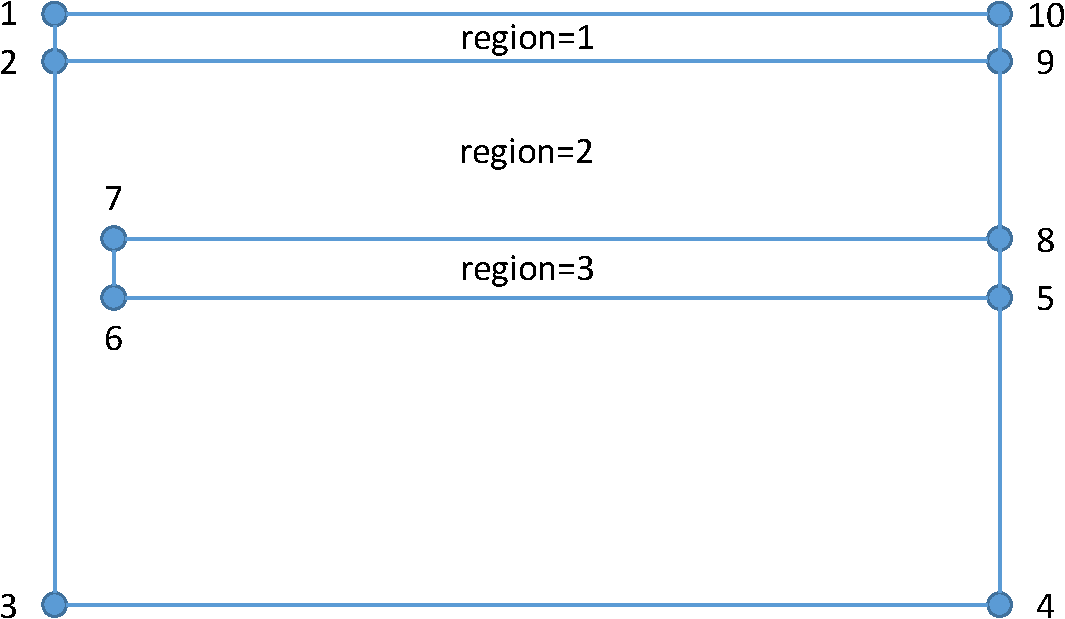
\includegraphics[scale=0.6]{ex_multilayer-crop.pdf}
\caption{Geometry of the multilayer example. Lengths are not to scale. The
point and region indices are indicated.}
\label{fig:multilayer}
\end{figure}

Here, three regions are defined (\texttt{nr=3} on the \texttt{\&setup} record,
three \texttt{\&material} and four \texttt{\&geometry} records). The geometry
defined by the input file is visualized in Fig.~\ref{fig:multilayer}. Since
\texttt{xinit} is not specified on the \texttt{\&ions} record, its default
value 0 is used. That means, all ions are implanted in the center of the target
at $x=0$, and their lateral straggle will not suffice for them to reach beyond
points 6 and 7 laterally.

In the definition of the material of region 2, the orientation of the crystal
with respect to the $x$ and $z$ axes is specified: The $z$ axis is parallel to
the [001] direction (\texttt{wafer=0.,0.,1.}), and the $x$ axis is parallel to
[110] (\texttt{vsurf=1.,1.,0.}).


% trick for having more than 1 crystalline layer

\section{Spot Burn}
This example shows the simulation of an ideally focused ion beam on a
crystalline Si target covered by a thin SiO$_2$ layer.

The input file reads:

\begin{verbatim}
B spot burn in 100-Si, 2 keV, 7 tilt, dose=1
 &setup    natom=3 nr=2 nion=1000000 nionhis=800 / 
 &ions     name='B' energy=2 dose=1 doseunits='1'
           tilt=7 diverg=0.3 /
 &material region=1 name='SiO2' xtal='no' /
 &material region=2 name='Si' xtal='yes' wafer=0,0,1 vsurf=1,0,0 /
 &snpar    lstffp=f /
 &damage   ldam=t lrcoil=t frec=0.3 ndamdim=3 /
 &geometry posif=0,10,10000 /
 &output   lmom=t lhis=t lhis2=t lhis3=t 
           nbox=200 wbox=10
           nbox2=100,50 wbox2=20,20 
           nbox3=0,0,0 wbox3=20,20,20 /
\end{verbatim}

The dose is specified as one ion (\texttt{dose=1 doseunits='1'} on the
\texttt{\&SETUP} record). This means that the 3-D histograms will represent the
probability density functions for the stop position of the ions, and for the
positions of the vacancies and interstitials. Since \texttt{xinit},
\texttt{yinit}, and \texttt{zinit} are not specified, these parameters assume
their default value \texttt{0}, so the reference point will be the origin of the
coordinate system for all ions.

Note that in this example the $x$ axis is parallel to the [100] crystal axis
(\texttt{vsurf=1,0,0} on the second \texttt{\&MATERIAL} record).
\texttt{ndamdim=3} on the \texttt{\&DAMAGE} record means that for dynamic damage
consideration the 3-D damage distribution will be taken into account (``damage
consideration'' means that atoms in the crystalline region are randomly
displaced, which normally results in a reduction of the channeling effect).
This corresponds to the actual situation in a spot burn. If \texttt{ndamdim=1}
were specified, a 1-D damage distribution would be taken into account derived from
the implant simulation. Damage-wise this would correspond to an implantation
with a homogeneous beam. The 3-D histograms would then correspond to the
probability density functions for one ion in a homogeneous beam.

On the \texttt{\&OUTPUT} record, output of 1-D, 2-D, and 3-D histograms are
requested. Only the 3-D histogram corresponds to the actual physical situation,
since the 3-D damage distribution is taken into account. The 1-D and 2-D
histograms are just convolutions of the 3-D histogram and do not correspond to
line or area implantations.

On the \texttt{\&OUTPUT} record, also the two possibilities for specifying the
box sizes of the histograms are demonstrated. For the 1-D and 2-D histograms,
\texttt{nbox} and \texttt{nbox2} are nonzero. This means that the number of
histogram boxes will never exceed the specified values. The box widths are
initialized with the values given by the \texttt{wbox} and \texttt{wbox}
parameter, respectively. The histogram is moved and/or the box widths are
doubled so that all entries are captured. In contrast, \texttt{nbox3=0}, which
means the histgram will always have the box widths specified by \texttt{wbox3},
and boxes will be added as to cover all entries.

% many output options

\section{Static Sputtering}
This example demonstrates a static sputtering simulation of Si by Ar ions.
``Static'' means that the target is not modified during the simulation.

The input file reads:

\begin{verbatim}
Sputtering of a-Si, static mode
Ar on a-Si, 10keV, 60 tilt
 &setup    ndim=1 natom=2 nr=1 ldyn=f lsput=t /
 &ions     name='Ar' energy=10 dose=1 tilt=60 diverg=0
           nion=100000 /
 &material region=1 name='Si' xtal='no' /
 &snpar    chkffpcyl=t /
 &damage   lrcoil=t esurf=4.1 ed=15 /
 &geometry posif=0,1000 /
 &output   lhis=t wbox=20 nbox=200 lmomab=t lhisab=t wboxa=1 /
\end{verbatim}

On the \texttt{\&setup} record, \texttt{lsput=t} is specified, indicating that
accurate sputtering simulation is requested. On the \texttt{\&damage} record,
the surface binding energy and the displacement energy are specified. Since
accurate sputtering simulation is requested, free flight paths will be chosen
such that no recoils with energy larger than the surface binding energy are
disregarded near the surface. Deeper in the bulk, larger free flight paths are
chosen, as recoils with energy up to the displacement energy can be neglected.

The sputter yield is written to the \texttt{OUT} file. In addition, the angular
distribution of the backward sputtered atoms is written to the \texttt{HISAB}
file (\texttt{lhisab=t}). The box width of the histogram is 1\textdegree\
(\texttt{wboxa=1}).

% Ar

\section{Dynamic Sputtering}
This example demonstrates a dynamic sputtering simulation of Si by Kr ions. In
this simulation, the target is modified as the ions bombard the target. To store
the state of the target at intermediate times, simulations are run repeatedly,
each simulation reading in the output of the previous one. When starting the
simulations with \texttt{mimsil.py}, the \texttt{-p} option must specify the
number of parallel processes to equal \texttt{1} (which is the default) in
order that the simulations run in sequence. Note that the order of the
simulations as specified in the parameters file is followed for \texttt{-p 1}.

The template file reads:

\begin{verbatim}
2 keV Kr in Si, tilt=60
 &setup    ndim=1 natom=2 nr=1 ldyn=t lsput=t
           usecell=#usecell# cellfile='#cellfile#' /
 &ions     name='Kr' energy=2 dose=1e15 tilt=60 diverg=0 nion=#nion# /
 &material region=1 name='Si' xtal='no' /
 &snpar    ef=4.7 denffp=4.7 /
 &damage   lrcoil=t ldam=f ed=15. frec=1 /
 &damage   atom1=1 esurf=0.1 /
 &separ    xnl=0. corlin=1. facscr=1. /
 &geometry posif=0,200 wrough=2 nionupd=100 posfix=190 fracupd=0. /
 &output   lhis=t lmomne=t lmomb=t lmomt=f lcell=t wbox=1 nbox=205 /
\end{verbatim}

Here we demand dynamic simulation by setting \texttt{ldyn=t} on the
\texttt{\&setup} record. As in the static sputtering simulation,
\texttt{lsput=t} is set to invoke accurate models for sputtering.

In order to read the results of the previous simulation, the \texttt{usecell}
and \texttt{cellfile} parameters are used on the \texttt{\&setup} record. The
value of \texttt{usecell} must be a variable, since in the first simulation
there is no cell file to be read, so \texttt{usecell=f} has to be used, while
\texttt{usecell=t} must be specified for the subsequent simulations. The value
of \texttt{cellfile} must be a variable, too, since the name of the cell file to
be read changes from simulation to simulation.

In order that the cell file is written, \texttt{lcell=t} is specified on the
\texttt{\&output} record.

There are two \texttt{\&damage} records. The first applies to all atoms. It is
important to specify \texttt{lrcoil=t} here in order to allow a sputtering
simulation. The second \texttt{\&damage} record applies only to atom 1, i.e.,
the first (and only) ion atom, Ar. Its surface binding energy is set to
0.1~eV. Such a low value leads to slow simulations, since all recoils down to
0.1~eV must be simulated; very short free flight paths and large impact
parameters must therefore be used. The motivation of this setting is that Ar
atoms close to the surface may leave the target easily.

On the \texttt{\&geometry} record, \texttt{wrough=2} specifies a 2~\AA\ thick
roughness layer. \texttt{nionupd=100} specifies that after every 100 simulated
ions relaxation of the target densities is attempted (an actual update is made
only if the relative change in any cell density exceeds \texttt{FRACUPD}).

\begin{verbatim}
def get_params(param):
    fname = 'krdyn_1e15'
    param[fname] = {}
    param[fname]['usecell'] = 'f'
    param[fname]['cellfile'] = ''
    param[fname]['nion'] = '1000'
    
    for dose in range(2,10):
        fname = 'krdyn_' + str(dose) + 'e15'
        param[fname] = {}
        param[fname]['usecell'] = 't'
        param[fname]['cellfile'] = 'krdyn_' + str(dose-1) + 'e15.cell'
        param[fname]['nion'] = '1000'
    
    fname = 'krdyn_10e15'
    param[fname] = {}
    param[fname]['usecell'] = 't'
    param[fname]['cellfile'] = 'krdyn_9e15.cell'
    param[fname]['nion'] = '10000'
\end{verbatim}

The parameters file is written as a Python function in order to allow a Python
loop to implement the loop over the simulations. The first simulation must be
kept separate as there is no cell file to be read. The last simulation is also
kept separate in order to obtain better statistics for the final results
(assuming sputter equilibirium has been reached). Note that \texttt{fname}
defines the file names of the input and output files (without extension). It is
made different for each simulation by the inclusion of the cumulated ion dose.

% krdyn

\section{RBS}
This example shows the input file for the simulation of an RBS/C spectrum
of a 1 $\mu$m thick (100) crystalline silicon membrane with a damage profile
defined in a histogram input file. 3~MeV He ions aligned with the [001]
direction are used.

\begin{verbatim}
RBS/C spectrum calculation  
He in <100> Si, 3000 keV, 0 Tilt, 3D interstitial
 &setup    nr=1 natom=2 
           atom1=2 atom2=2 ndim=1 usehis=t hisfile='dam2percent.his' /  
 &ions     name='He' energy=3000 dose=1e14 tilt=0.0 nion=10000 /
 &material region=1 name='Si' xtal='on' /
 &damage   ldam=t lamo2=f /
 &geometry posif=0,10000 /
 &output   lhis=t lrbs=t wboxe=6000. nboxe=0 tilta=10. / 
\end{verbatim}

The histogram file is read on the \texttt{\&setup} record (\texttt{usehis=t
hisfile='dam2percent.his'}). The \texttt{.his} file must conform to the format
of a 1-D histogram file (see Section~\ref{s:his1d}), and can of course be an
output histogram of another IMSIL run. In this case it has been created by hand
with a constant damage concentration of 2\% (not shown). Note that
\texttt{hisfile} must refer to the parent directory if IMSIL is run with the
\texttt{imsil.py} script, since this file is not copied into the subdirectory
where IMSIL is run. \texttt{atom1=2} indicates that the second atom stored in
the histogram file is to be read. \texttt{atom2=2} indicates that the damage
concentrations of atom 2 of the simulation are to be initialized with these
values.

\texttt{lamo2=f} on the \texttt{\&damage} record specifies that the 3-D random
interstitial model be used. In this model, the target atoms are displaced due to
lattice vibration according to a 3-D Gaussian probability density function. The
default is displacement in the plane perpendicular to the direction of motion
according to a 2-D Gaussian probability density function (\texttt{lamo2=f}),
which is computationally slightly more efficient.

Finally, \texttt{lrbs=t} on the \texttt{\&output} record causes an RBS file to
be written, see Section~\ref{s:his1d}. The energy box widths are 6000\AA. The
backscattering angle is specified as 170\textdegree\ (\texttt{tilta=10.}).


\ifprivate
\section{Example 2}
\footnote{This example is currently not functional.}
The following example shows the \texttt{INP} file for the simulation of an
RBS/C spectrum into a 1 $\mu$m thick (100) crystalline silicon with a damage
profile defined in a histogram input file. Damage is in the form of
split-$\langle 110 \rangle$ interstitials. The coordinates of the defects and
strained regions are taken from ab-initio calculations. A silicon cell
containing 1.6 million lattice atoms (10x10x2000 unit cells) is populated
according to the requested damage concentrations (defined in histogram file
\texttt{'hisfile'}) with required defect type (\texttt{FRACSPL=1.0}). Periodic
boundary conditions in lateral dimensions are applied. 3~MeV He$^+$ ions and a
backscattering angle of $170^\circ$ are used.  Recoils are not followed.

\begin{verbatim}
IMSIL test example2
RBS/C (100) spectra of 3 Mev He ions. 
 &setup    nr=1 natom=2 usehis=t hisfile='profile.his' 
           atom1=2 atom2=2 / 
 &ions     name='He' energy=3000 dose=1e14 ranrot=t 
           nion=100000 /
 &material region=1 name='Si' vsurf=1,1,0 wafer=0,0,1 xtal='yes' /
 &damage   ldam=t ldet=t fracspl=1.0 wcol=40,40,8000 /
 &geometry posif=0,10000 /
 &output   lrbs=t lhis=t ldef=t wboxei=6000. tilta=10. /
\end{verbatim}

As discussed in Chapter \ref{k:input}, the first two lines are comments and
have no further meaning. The third line
%
\begin{verbatim}
 &setup    nr=1 natom=2 usehis=t hisfile='profile.his' 
           atom1=2 atom2=2 / 
\end{verbatim}
%
specifies that there is 1 region and a total of 2 atom species (the He ion
plus the Si target atoms, see below).  The damage profile is read from the
histogram file \texttt{profile.his} (\texttt{usehis=t, hisfile='profile.his'}.
The histogram file can be the output of a previous simulation or can be
created separately, with a format defined in Chapter \ref{k:files}. The atom
index \texttt{ATOM1=2} (column number three) corresponds to atom index in the
histogram file which will be used to initialize atom index index 2
\texttt{ATOM2=2}, which is in this case silicon. The next line
%
\begin{verbatim}
 &ions     name='He' energy=3000 dose=1e14 ranrot=t
           nion=100000 /
\end{verbatim}
%
defines the properties of the ions: The ion species is He, the energy
3000~keV, the dose $10^{14}~$cm$^{-2}$, the tilt angle is $0^\circ$ (default
value) and random rotation of ions is used. 100000 projectiles are requested
to be simulated.  The next record
%
\begin{verbatim}
 &material region=1 name='Si' vsurf=1,1,0 wafer=0,0,1 xtal='yes' /
\end{verbatim}
%
specifies the material of the target region as single-crystal (100)-Si 
(\texttt{wafer=0,0,1}).

The next record,
%
\begin{verbatim}
 &damage   ldam=t ldet=t fracspl=1.0 wcol=40,40,8000 /
\end{verbatim}
%
specifies that damage in the crystalline region shall be taken into account
dynamically for the simulation of subsequent trajectories, that the
deterministic model of damage is used, and that the defect type is always
split-$\langle 110 \rangle$ interstitials (\texttt{FRACSPL=1.0}). Since we use
the histogram damage profile \texttt{USEHIS=T} the simulation cell with size
of 10x10x2000 unit cells (notice that the input units for \texttt{WCOL} are a
quarter of the lattice constant) will be populated with
split-$\langle110\rangle$ interstitials \texttt{FRACSPL=1} according to
concentration profile specified with atom index 2 \texttt{ATOM1=2} in
histogram file \texttt{'profile.his'}.

Since there are no \texttt{\&xtal} \texttt{\&snpar}, or \texttt{\&separ}
records, the default parameters for the crystal, nuclear, and electronic
stopping are used.

The next input record
%
\begin{verbatim}
 &geometry posif=0,10000 /
\end{verbatim}
%
specifies that the target geometry is a 1-D layered structure (the default value
of \texttt{ndim} in the \texttt{\&setup} record is \texttt{1}). The Si layer (as
specified in the \texttt{\&material} record) extends from $z=0$ to
$z=10000$\AA\ ($=1~\mu$m). Finally,
%
\begin{verbatim}
 &output lrbs=t lhis=t ldef=t wboxei=6000. tilta=10. /
\end{verbatim}
%
specifies the RBS energy spectrum box width wboxei=6000.\texttt{eV}. The RBS
backscattering angle is $170^\circ$. Notice that when \texttt{LRBS=T} is set the
angle is calculated as $\texttt{$180^\circ$} - \texttt{TILTA}$ which gives
$180^\circ - 10^\circ = 170^\circ$). Requested output files are: 1-D
histograms of the dopants and the damage into the \texttt{HIS} file,
RBS/S spectra into the \texttt{RBS} file and deterministic defects into the
\texttt{DEF} file.

If the script delivered with the program is used, the input file could be
named \texttt{he3mev.inp}. IMSIL would produce the files \texttt{he3mev.out},
\texttt{he3mev.his}, \texttt{he3mev.rbs}, and \texttt{he3mev.def}.


\fi
%
%%%%%%%%%%%%%%
% Literature %
%%%%%%%%%%%%%%
%
%\input{ref.tex}
\bibliography{manual,imsil}
%
\nociteimsil{hobler_efficient_1987}
\nociteimsil{hobler_two-dimensional_1988}
\nociteimsil{hobler_monte_1989}
\nociteimsil{hobler_empirical_1991}
\nociteimsil{hobler_simulation_1991}
\nociteimsil{hobler_two-dimensional_1991}
\nociteimsil{hobler_effect_1992}
\nociteimsil{hobler_electronic_1993}
\nociteimsil{hobler_role_1993}
\nociteimsil{simionescu_monte_1994}
\nociteimsil{gartner_round_1995}
\nociteimsil{herzog_monte_1995}
\nociteimsil{hobler_boron_1995}
\nociteimsil{hobler_monte_1995}
\nociteimsil{simionescu_comparison_1995}
\nociteimsil{simionescu_modeling_1995}
\nociteimsil{simionescu_model_1995}
\nociteimsil{simionescu_monte_1995}
\nociteimsil{hobler_acceleration_1995}
\nociteimsil{hobler_critical_1996}
\nociteimsil{hobler_net_1996}
\nociteimsil{hobler_theoretical_1996}
\nociteimsil{hobler_verification_1996}
\nociteimsil{hobler_modeling_1997}
\nociteimsil{hobler_study_1997}
\nociteimsil{nikulin_model-independent_1997}
\nociteimsil{criegern_verification_1998}
\nociteimsil{hobler_channeling_1999}
\nociteimsil{hobler_continuum_1999}
\nociteimsil{hobler_modeling_1999}
\nociteimsil{hobler_dose_2000}
\nociteimsil{hobler_towards_2000}
\nociteimsil{boxleitner_fibsim_2001}
\nociteimsil{boxleitner_dynamic_2001}
\nociteimsil{hobler_initial_2001}
\nociteimsil{hobler_useful_2001}
\nociteimsil{palmetshofer_range_2001}
\nociteimsil{hobler_amorphous_2003}
\nociteimsil{hobler_simulation_2003}
\nociteimsil{hobler_status_2003}
\nociteimsil{lugstein_method_2003}
\nociteimsil{otto_coupled_2003}
\nociteimsil{otto_dose-rate_2005}
\nociteimsil{kovac_modeling_2005}
\nociteimsil{hobler_multiscale_2005}
\nociteimsil{otto_coupled_2005}
\nociteimsil{zahel_atomistic_2005}
\nociteimsil{hobler_random_2006}
\nociteimsil{kovac_investigation_2006}
\nociteimsil{otto_is_2006}
\nociteimsil{kim_simulation_2007}
\nociteimsil{otto_amorphous_2007}
\nociteimsil{ebm_simulation_2009}
\nociteimsil{ebm_assessment_2009}
\nociteimsil{ebm_ion_2009}
\nociteimsil{kovac_amorphous_2009}
\nociteimsil{ebm_quantitative_2011}
\nociteimsil{hobler_dynamic_2011}
\nociteimsil{kim_sputter-redeposition_2011}
\nociteimsil{kim_simulation_2012}
\nociteimsil{lindsey_significance_2012}
\nociteimsil{hobler_assessment_2013}
\nociteimsil{lindsey_sputtering_2013}
\nociteimsil{lindsey_inverse_2014}
\nociteimsil{hobler_combined_2015}
\nociteimsil{hobler_probing_2016}
\nociteimsil{hobler_sputtering_2016}
\nociteimsil{lindsey_simple_2017}
\nociteimsil{g._hobler_simulation_2018}
\nociteimsil{hobler_crater_2018}
\nociteimsil{m._current_channeled_2018}
\nociteimsil{urbassek_sputtering_2018}
\nociteimsil{hobler_channeling_2019}
\nociteimsil{hobler_ion_2019}
\nociteimsil{m._current_aspects_2019}
\nociteimsil{schlueter_absence_2020}
\nociteimsil{bradley_second_2021}

\bibliographyimsil{imsil}
%
\end{document}
